\documentclass[11pt, oldfontcommands, oneside, a4paper]{memoir}
\usepackage{etoolbox}

\newtoggle{dutch}
\toggletrue{dutch}

\iftoggle{dutch} {
	\def \langPath {nl/}
}{	
  \def \langPath {en/}
}

\usepackage[T1]{fontenc}
\usepackage{import}
\usepackage{media9} 
\usepackage{amssymb} % for changing item bullets
\usepackage{bbding} % dingbats (for bullets)
\usepackage{textcomp}
\usepackage{color,calc,graphicx,soul}
\usepackage{geometry}
\usepackage{layout}
\RequirePackage[calcwidth]{titlesec}
\usepackage{bookman}
\usepackage{fix-cm}
\let\footruleskip\undefined %will be redefined in fancyhdr
\usepackage{fancyhdr}
\usepackage[bookmarks, colorlinks=true]{hyperref}
\usepackage{makeidx}
\usepackage{hyphenat}
\usepackage{parskip}
\usepackage[most]{tcolorbox}
\usetikzlibrary{shadows}
\usepackage{environ}
\usepackage{polyglossia}
\usepackage{listings,fontspec}


\geometry{
	includeheadfoot,
	margin=2.54cm
}

%% colors 
\definecolor{primaryBack}{HTML}{4782D3}
\definecolor{primaryDark}{HTML}{14478D}
\definecolor{primaryLight}{HTML}{98BEF4}
\definecolor{primaryIntense}{HTML}{2965B9}

\definecolor{secondaryBack}{HTML}{FF8145}
\definecolor{secondaryDark}{HTML}{D64E0D}
\definecolor{secondaryLight}{HTML}{FFB795}
\definecolor{secondaryIntense}{HTML}{FF6C25}

\definecolor{thirdBack}{HTML}{FFDC45}
\definecolor{thirdDark}{HTML}{D6B00D}
\definecolor{thirdLight}{HTML}{FFEB95}
\definecolor{thirdIntense}{HTML}{FFD625}

\definecolor{complementBack}{HTML}{FFB945}
\definecolor{complementDark}{HTML}{D68A0D}
\definecolor{complementLight}{HTML}{FFD795}
\definecolor{complementIntense}{HTML}{FFAD25}

\definecolor{hidden}{HTML}{FFD7B5}

\definecolor{red}{HTML}{FF0000}
\definecolor{blue}{HTML}{0000FF}
\definecolor{green}{HTML}{009900}
\definecolor{orange}{HTML}{FFA500}
\definecolor{black}{HTML}{000000}

% section header
\titleformat{\section}[hang]{\bfseries}{
\huge\color{primaryIntense}\thesection}{10pt}{\huge\raggedleft\color{primaryIntense}}[{\titlerule[0.5pt]}]

% subsection header
\titleformat{\subsection}[hang]{\bfseries}{
\huge\color{primaryIntense}\thesubsection}{10pt}{\LARGE\raggedleft\color{primaryIntense}}
\setcounter{secnumdepth}{3}

% subsection header
\titleformat{\subsubsection}[hang]{\bfseries}{
\large\color{primaryIntense}\thesubsubsection}{10pt}{\large\raggedleft\color{primaryIntense}}


% table of contents
\pagestyle{fancy}
\hypersetup{linkcolor=primaryDark}
\maxtocdepth{subsubsection}

% colored description
%\setdescription{leftmargin=1cm,labelindent=0.4cm}
%\renewcommand{\descriptionlabel}[1]
%{\hspace{\labelsep}{\color{red}{\bfseries #1}}}
%
% color of texttt
\let\Oldtexttt\texttt
\renewcommand\texttt[1]{{\ttfamily\color{primaryDark} {\bfseries #1}}}

% chapter header
\makeatletter
\newlength\dlf@normtxtw
\setlength\dlf@normtxtw{\textwidth}
\def\myhelvetfont{\def\sfdefault{mdput}}
\newsavebox{\feline@chapter}
\newcommand\feline@chapter@marker[1][4cm]{%
\sbox\feline@chapter{%
\resizebox{!}{#1}{\fboxsep=1pt%
\colorbox{primaryBack}{\color{complementIntense}\bfseries\sffamily\thechapter}%
}}%
\rotatebox{90}{%
\resizebox{%
\heightof{\usebox{\feline@chapter}}+\depthof{\usebox{\feline@chapter}}}%
{!}{\scshape\so\@chapapp}}\quad%
\raisebox{\depthof{\usebox{\feline@chapter}}}{\usebox{\feline@chapter}}%
}
\newcommand\feline@chm[1][4cm]{%
\sbox\feline@chapter{\feline@chapter@marker[#1]}%
\makebox[0pt][l]{% aka \rlap
\makebox[1cm][r]{\usebox\feline@chapter}%
}}
\makechapterstyle{daleif1}{
\renewcommand\chapnamefont{\normalfont\Large\scshape\raggedleft\so}
\renewcommand\chaptitlefont{\normalfont\huge\bfseries\scshape\color{primaryIntense}}
\renewcommand\chapternamenum{}
\renewcommand\printchaptername{}
\renewcommand\printchapternum{\null\hfill\feline@chm[2.5cm]\par}
\renewcommand\afterchapternum{\par\vskip\midchapskip}
\renewcommand\printchaptertitle[1]{\chaptitlefont\raggedleft ##1\par}
}
\makeatother
\chapterstyle{daleif1}

%title page
\makeatletter
\newlength\drop
\newcommand*{\titleGM}{%
	\thispagestyle{empty}
	\begingroup% Gentle Madness
	\drop = 0.1\textheight
	\vspace*{\baselineskip}
	\hbox{%
		\hspace*{0.2\textwidth}%
		\hspace*{0.05\textwidth}% 
		\parbox[b]{0.75\textwidth}{%
		   \vbox{%
				 \vspace{\drop}
				 \rule{0.75\textwidth}{1pt}
				 {\Huge\bfseries\sffamily\raggedleft\color{primaryIntense}\@title\par}
				 \vskip2.37\baselineskip
				 {\Large\bfseries\sffamily\raggedleft\color{primaryDark}\@author\par}
				 \rule{0.75\textwidth}{1pt}
				 \vskip4.37\baselineskip
				 {\Large\bfseries\sffamily\raggedleft\color{primaryDark}Revision: \@date\par}
				 \vskip4.37\baselineskip
				 
\includegraphics[scale=0.2]{mute-logo}
			 }
		}
	}
	\pagebreak
	\vfill
	\null
	\endgroup
}
\makeatother

%part page
\makeatletter

\renewcommand\printpartname{}
\renewcommand\printpartnum{}
\renewcommand{\parttitlefont}{\normalfont\raggedleft\Huge\scshape\color{primaryIntense}}
\newcommand{\partAbstract}[1]{\gdef\@partAbstract{\leftskip5em\normalsize\color{black}\textit{#1}}}
\renewcommand{\printparttitle}[1]{%
\raggedleft
\rule{0.75\textwidth}{1pt}
\vskip1.37\baselineskip
\parttitlefont Part \thepart: #1
\color{black}
\rule{0.75\textwidth}{1pt}
\vskip1.37\baselineskip
\@partAbstract\vfil
}
\makeatother

%paragraph
\setlength{\parindent}{0pt}
\setlength{\parskip}{0.5cm plus3mm minus2mm}

%table

\newcommand{\tempcaption}{}
\newenvironment{myTable}[2]{%
  \gdef\tempcaption{#1}%
  \begin{center}%

    \begin{tcolorbox}[
      colback=primaryLight,
      colframe=primaryIntense,
      left=1mm,right=1mm,top=1mm,bottom=1mm,boxsep=0mm,
      toptitle=0.5mm,
      bottomtitle=0.5mm,
      center title,
      title=\tempcaption,
    ]%
    \centering
    \begin{tabular}{#2}%
}{%
    \end{tabular}%
    \end{tcolorbox}%
  \end{center}%
}

%listing
\lstset{
  frame=tb,
  language=c++,
  aboveskip=3mm,
  belowskip=3mm,
  showstringspaces=false,
  columns=flexible,
  basicstyle={\small\ttfamily},
  %backgroundcolor=\color{primaryLight}, % Set the background color for the snippet - useful for highlighting
  firstnumber=1, % Line numbers begin at line 1
  stepnumber=5,
  frame=lines, % Frame around the code box, value can be: none, leftline, topline, bottomline, lines, single, shadowbox
  %frameround=tttt, % Rounds the corners of the frame for the top left, top right, bottom left and bottom right
  numbers=left,
  numbersep=10pt, % Distance of line numbers from the code box
  numberstyle=\tiny\color{primaryDark}, % Style used for line numbers
  rulecolor=\color{primaryDark}, % Frame border color
  keywordstyle=\color{blue},
  commentstyle=\color{green},
  stringstyle=\color{red},
  breaklines=true,
  breakatwhitespace=true,
  tabsize=2
}

\lstset{
  emph={Vec, Vec2, Circle, Memc, Str, FREPA, SQLColumn, SQLValues, TextData, File, 
	      Memx, SQL, GuiObjs, Window, Button, TextLine, TextNode},
  emphstyle={\color{blue}\bfseries}
}

\renewcommand{\labelitemi}{\SquareShadowBottomRight}
\renewcommand{\labelitemii}{\tiny\Square}

% special blocks
\newtheorem{example}{Example}
\newtheorem{remember}{Remember This!}

\tcbset{
myNote/.style={
  enhanced,
  colback=complementLight,
  colframe=complementDark,
  fonttitle=\scshape,
  title={Note},
  title style={fill=complementDark},
  }
}

\newtcolorbox{note}{myNote}

\tcbset{
myInfo/.style={
  enhanced,
  colback=complementLight,
  colframe=complementDark,
  fonttitle=\scshape,
  title={Info},
  title style={fill=complementDark},
  }
}

\newtcolorbox{info}{myInfo}

%\tcbset{
%myWorld/.style={
  %enhanced,
  %colback=thirdLight,
  %colframe=thirdIntense,
  %fonttitle=\scshape,
  %title={De echte wereld},
  %title style={fill=thirdDark},
  %coltitle=thirdLight,
  %}
%}
%
%\newtcolorbox{praktijk}{myWorld}

\tcbset{
myWarning/.style={
  enhanced,
  colback=thirdLight,
  colframe=thirdIntense,
  fonttitle=\scshape,
  title={Warning!},
  title style={fill=thirdDark},
  coltitle=thirdLight,
  }
}

\newtcolorbox{warning}{myWarning}

\tcbset{
myExercise/.style={
  enhanced,
  colback=primaryLight,
  colframe=primaryDark,
  fonttitle=\scshape,
  title={Time for Action},
  title style={fill=primaryDark},
  }
}

\newtcolorbox{exercise}{myExercise}

\newcommand*\tick{\item[\Checkmark]}
\newcommand*\fail{\item[\XSolidBrush]}
\newcommand*\pencil{\item[\PencilRightDown]}

\tcbset{
myTest/.style={
  enhanced,
  colback=secondaryLight,
  colframe=secondaryDark,
  fonttitle=\scshape,
  fontlower=\itshape,
  title={Test Jezelf},
  title style={fill=secondaryDark},
  collower=hidden,
  }
}

\newtcolorbox{test}{myTest}

\lstnewenvironment{code}
	{
		\lstset{language={[Visual]C++}, columns=fixed}
	}
	{
	}
%
\newcommand{\eeClass}[1]{\texttt{#1}}
\newcommand{\eeFunc}[1]{\texttt{#1}}
\newcommand{\eeOpp}[1]{\texttt{#1}}

\author{Mute (http://mutecode.com)}

\graphicspath{ {images/} }



\title{Learning C++ with Esenthel}
\begin{document}
\titleGM
\tableofcontents

%\mode<all>
%%\part{C++ en Esenthel}
%%\chapter{Gui}

Een grafische user interface (Gui) kan je visueel ontwerpen via de gui editor. Maar om je interface te gebruiken in je applicatie zal je wel moeten programmeren.
Bekijk eerst hoe je de gui editor gebruikt. Je kan daarvoor gebruik maken van deze youtube tutorial:

\url{https://www.youtube.com/watch?v=eFsBxC6pGxE}

\section{Een gui laden}

Voor elk window maak je best een afzonderlijk code bestand, dat houdt het overzichtelijk. In dat bestand begin je een class, die bij voorkeur dezelfde naam heeft als de Gui en het bestand. 

\begin{code}
// Een class voor een login window
class loginWindow
{
private:
	 // een GuiObjs object kan een Gui object bevatten
	 // dat je maakt via de editor.
   GuiObjs objs;
   
public:
   // Deze create functie zullen we later in het programma
	 // uitvoeren om het login window te laden.
   void create()
   {
	    // het GuiObjs object kan je gebruiken om een gui te
			// laden. Met de functie load kan je hier via drag and 
			// drop een GUI object plaatsen.
      objs.load( --- Drop Gui Object here --- );
      
			// Uiteindelijk voeg je deze gui toe aan de Gui Manager
      Gui += objs;
   }
   
}

// aangezien je normaal gezien maar 1 object nodig hebt van elke gui class,
// kan je dat hier al maken.
loginWindow LoginWindow;
\end{code}

De bovenstaande code laad je gui in het geheugen en voegt die toe aan de Gui manager. In je programma ga je dan de \texttt{create()} functie uitvoeren en de Gui updaten en tekenen.

\begin{code}
void InitPre()
{
   EE_INIT();
}

bool Init()
{
   // voor elk gui object voer je de create functie uit
   // tijdens de Init fase
   LoginWindow.create();
   return true;
}

void Shut() {}

bool Update()
{
   // Wanneer je een of meerdere gui classes gebruikt, dan 
   // update je de Gui manager tijdens de applicatie update
   Gui.update();
   return true;
}

void Draw()
{
   D.clear(WHITE);
   
   // Wanneer je een of meerdere gui classes gebruikt,  dan
   // laat je de Gui manager alles op het scherm tekenen. Je
   // doet dit op het einde van de Draw functie,  omdat de 
   // de Gui boven op de andere objecten hoort.
   Gui.draw();
}
\end{code} 

\begin{exercise}
Maak een login window (met naam, wachtwoord textlines en een ok en cancel button) en zorg via bovenstaande code dat het in een programma op je scherm verschijnt.
\end{exercise}

\section{Pointers naar elementen}
Je hebt nu wel een gui geladen, maar je wil waarschijnlijk ook de elementen van de gui gebruiken. Maar die zitten in \texttt{GuiObjs objs}. Je maakt daarom pointers aan naar elk element waar je iets mee wil doen. Na het laden van de gui zoek je naar de elementen en wijs je die toe aan de gewenste pointer.

\begin{code}
class loginWindow
{
private:
   GuiObjs objs;
	 // een pointer naar een Window, met de naam window
	 Window * window;
	 // een pointer naar een Button, met de naam buttonClose
	 Button * buttonClose;
   
public:

   void create()
   {
      objs.load( --- Drop Gui Object here --- );
			// zoek in objs naar een Window met de naam "window"
      window = objs.findWindow("window");
			// zoek in objs naar een Button met de naam "buttonClose"
			buttonClose = objs.findButton("buttonClose");
			
      Gui += objs;
   }
   
}
loginWindow LoginWindow;
\end{code}

Je mag je elementen noemen zoals je wil, maar de naam waar je naar zoekt (met findWindow, findButton, \ldots) moet wel gelijk zijn aan de naam die je het element in de Gui Designer hebt gegeven. Als je toch een verkeerde naam zoekt, dan zal je pointer nergens naar verwijzen. Als je dan later die pointer gebruikt in het programma, dan zal je applicatie crashen.

Eens een pointer verwijst naar een element, kan je hem gebruiken in je code. Het volgende voorbeeld gebruikt de pointer naar het window om dit te tonen en te verbergen:

\begin{code}
class loginWindow
{
private:
   GuiObjs objs;
	 Window * window;
	 Button * buttonClose;
   
public:

   void create()
   {
      objs.load( --- Drop Gui Object here --- );
      window = objs.findWindow("window");
			buttonClose = objs.findButton("buttonClose");
			
			// verberg het window na het laden
			window.hide();
			
      Gui += objs;
   }
	
	 // deze functie kan je eender waar in je programma gebruiken
	 void show() {
			// dit zorgt voor een fade in van je window	
	    window.fadeIn();
   }
}
loginWindow LoginWindow;
\end{code}

De bovenstaande code laat je toe om bijvoorbeeld in de update functie van je applicatie de volgende code te plaatsen:

\begin{code}
if(Kb.bp(KB_F5)) LoginWindow.show();
\end{code}

\section{Callback functies}
Sommige gui elementen, zoals buttons, kan je een functie toewijzen. Die functie wordt dan automatisch uitgevoerd bij een actie. Bij een button is die actie het moment dat iemand klikt op de button. Bij een slider is het het moment waarop de slider verplaatst wordt. Een TextLine heeft dan weer een actie als iemand de waarde aanpast.

De functie die je toewijst aan een element kan eender welke naam hebben, maar het formaat moet wel juist zijn. Je moet de functie declareren als \texttt{static void} en met als argument een referentie naar de class die je maakt. Bijzonder aan een \texttt{static} functie is dat die geen rechtstreekse toegang heeft tot de objecten in je class. Daarom is de referentie naar de class noodzakelijk. Wanneer je de functie doorgeeft aan de button, gebruik je \eeClass{T} om het object door te geven waar de functie bij hoort. Andere functies of elementen van de class moet je dus ook via die referentie benaderen.

\begin{code}
class loginWindow
{
private:
   GuiObjs objs;
	 Window * window;
	 Button * buttonClose;
    
	 // Deze functie wordt uitgevoerd wanneer iemand
	 // op de button klikt.
   static void myButtonFunction(loginWindow & obj) {
		  obj.window.fadeOut();
	 }
	
public:

   void create()
   {
      objs.load( --- Drop Gui Object here --- );
      window = objs.findWindow("window");
			buttonClose = objs.findButton("buttonClose");
			window.hide();
			
			// Wijs de functie hierboven toe aan de button
			buttonClose.func(myButtonFunction, T);
      Gui += objs;
   }
	
	 void show() {
	    window.fadeIn();
   }
}
loginWindow LoginWindow;
\end{code}

\begin{note}
Pas op. De editor maakt een fout als je de naam van een functie typt: er komen vanzelf haakjes achter. Wanneer je een functie gebruikt hoort dat zo, maar in dit geval moet je enkel de naam doorgeven. Verwijder de haakjes dus.
\begin{code}
buttonClose.func(myButtonFunction(), T); // fout!
buttonClose.func(myButtonFunction, T);   // juist.
\end{code}
\end{note}
(
\begin{exercise}
Vul de vorige oefening aan met de mogelijkheid om je login window te tonen en te verbergen via de functietoets F1. Zorg ook dat zowel de ok als de cancelbutton het window terug sluiten.
\end{exercise}

\section{De inhoud van een element}
\label{chapter:gui_content}
Dikwijls heeft een element ook een inhoud. Een \texttt{TextLine} heeft een tekst als inhoud. Een \texttt{Slider} heeft een waarde tussen 0 en 1, afhankelijk van zijn positie. Een \texttt{CheckBox} heeft als inhoud \texttt{true} wanneer aangevinkt, of \texttt{false} indien niet. 

Die inhoud opvragen kan complex zijn. Stel je voor dat we een \texttt{TextLine} hebben:

\begin{code}
TextLine tl;
\end{code}

De waarde vragen vraag je dan op met:

\begin{code}
Str waarde = tl();
\end{code}

Eenvoudig! Maar\ldots\ meestal hebben we geen \texttt{TextLine} in onze code, maar een \textbf{pointer} naar zo'n element. Dus moet je aangeven dat je wil werken met het element waar die pointer naar verwijst. Dat kan zo:

\begin{code}
Str waarde = (*tl)();
\end{code}

Als je dan ook nog eens vanuit een \texttt{static void} functie werkt, zoals een functie die wordt uitgevoerd wanneer je op een knop klikt, dan moet je ook het object van de class meegeven. Bij de class \texttt{loginWindow} van hierboven wordt dat dan:

\begin{code}
Str waarde = (*LoginWindow.tl)();
\end{code}

Je kan de inhoud van een element ook wijzigen. Dat is gelukkig een stuk eenvoudiger:

\begin{code}
Str waarde = "mijn tekst";
tl.set(waarde);
// of in een static void functie
LoginWindow.tl.set(waarde);
\end{code}

Een verder uitgewerkt voorbeeld van het loginWindow zou er zo kunnen uitzien:

\begin{code}
class loginWindow
{
private:
   GuiObjs objs;
	 Window * window;
	 Button * buttonLogin;
   TextLine * tlName;
	 TextLine * tlPass;
	
   static void tryLogin(loginWindow & obj) {
	    Str name = (*obj.tlName)();
			Str pass = (*obj.tlPass)();
			
			if(Equal(name, "john") && Equal(pass, "secret")) {
			   obj.window.fadeOut();
		  }
	 }
	
public:

   void create()
   {
      objs.load( --- Drop Gui Object here --- );
      window = objs.findWindow("window");
			buttonLogin = objs.findButton("login");
			tlName = objs.findTextLine("name");
			tlPass = objs.findTextLine("pass");
			
			window.hide();
			buttonClose.func(tryLogin, T);
			
      Gui += objs;
   }
	
	 void show() {
	    window.fadeIn();
   }
}
loginWindow LoginWindow;
\end{code}

\begin{exercise}
Maak een programma met een login window. De achtergrond van het programma is zwart, maar wordt wit wanneer je ingelogd bent. Je toont dan ook de login naam op het scherm via \texttt{D.text()}. Als uitbreiding kan je ook eens naar een andere application state overschakelen na het inloggen.
\end{exercise}

\section{Data en interface: Never mix!}
Een belangrijke regel bij het schrijven van een GUI is de volgende:

\begin{note}
GUI en data houd je strikt gescheiden.
\end{note}

Een GUI dient om data aan te passen. Maar die data zelf hoort \textbf{NOOIT} (nooit) thuis in de gui class. Je maakt dus steeds een afzonderlijke class voor de data. Je gebruikt dan functies in je gui class om die data te lezen en te wijzigen. Een voorbeeld:

\begin{code}
// een data class voor een player
class player {
private:
   Str name;
	 int age;

public:
   void setName(C Str & name) { T.name = name; }
	 void setAge (int     age ) { T.age  = age ; }
	 Str  getName(            ) { return   name; }
	 int  getAge (            ) { return   age ; }
	
	 void draw() {
	    D.text(0,    0, S + "name: " + name);
			D.text(0, -0.1, S + "age : " + age );
	 }
}
player Player;
\end{code}

\begin{code}
// een GUI class
class changePlayerGUI {
private:
   GuiObjs objs;
	 Window   * window  ;
	 TextLine * tlName  ;
	 TextLine * tlAge   ;
	 Button   * buttonOK;
	
public:
   void create() {
	    objs.load( -- drop gui object here ---);
			window   = objs.findWindow  ("window");
			tlName   = objs.findTextLine("name"  );
			tlAge    = objs.findTextLine("age"   );
			buttonOK = objs.findButton  ("ok"    );
			
			buttonOK.func(changeData, T);
			tlName  .set(        Player.getName() );
			tlAge   .set(TextInt(Player.getAge ())); // converteer int naar Str met TextInt()
			
			Gui += objs;
   }
	
	 static void changeData(changePlayerGUI & obj) {
	    Str name = (*obj.tlName)();
	 	  Str age  = (*obj.tlAge )();
	 	  int ageInt = TextInt(age);
	 	  Player.setName(name  );
	 	  Player.setAge (ageInt);
   }
}

changePlayerGUI ChangePlayerGUI;
\end{code}


\part{2D Concepts}
\chapter{Posities in 2D}
\label{chapter:positions}

Posities in 2D hebben een x- en een y-co\"ordinaat, net zoals een punt in een grafiek. In Esenthel staat het nulpunt voor het midden van het scherm. Positieve waarden op de X-as staan rechts, negatieve waarden links. Positieve waarden op de Y-as staan bovenaan, negatieve waarden beneden.

\begin{figure}[h]
\centering
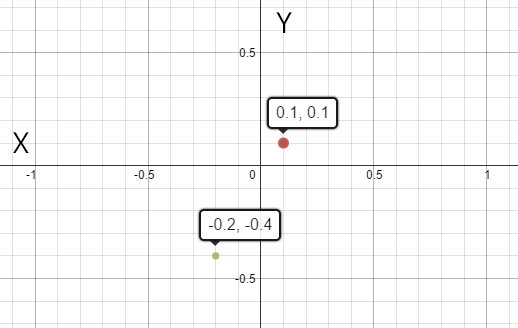
\includegraphics[width=0.7\linewidth]{../images/2Dpositions.png}
\caption[]{2D co\"ordinaten.}
\label{fig:pos2D}
\end{figure}

In Esenthel gebruiken we de class \texttt{Vec2} om een 2D co\"ordinaat weer te geven. Van een \texttt{Vec2} kan je zowel de x als de y waarde instellen:

\begin{code}
Vec2 pos;
pos.x =  0.1; // de positie op de x-as wordt 0.1
pos.y = -0.3; // de positie op de y-as wordt -0.3
pos   =  0.5; // beide assen krijgen de waarde 0.5
pos.set(0.1, -0.3); // pas beide assen aan via de functie set(float x, float y)
\end{code}

\begin{exercise}
Waar zouden deze posities zich op het scherm bevinden?
\end{exercise}

\section{Posities Tonen op het Scherm}

Alhoewel je de class \texttt{Vec2} vooral gebruikt om posities te berekenen, kan je een co\"ordinaat ook op het scherm tonen. Daarvoor bevat de class de functie \texttt{draw(Color)}. Als argument geef je de kleur waarin je je punt wil weergeven. 

\begin{code}
Vec2 p1(0.2, 0.4); // maak een punt p1 en stel x en y in via de constructor.
Vec2 p2;           // maak een punt p2.

void InitPre()
{
   EE_INIT();
}

bool Init()
{
   p2.set(-0.2, -0.5); // stel p2 in via de set functie
   return true;
}

void Shut() {}

bool Update()
{
   if(Kb.bp(KB_ESC)) return false;
   
   return true;
}

void Draw()
{
   D.clear(BLACK); // Maak het scherm leeg
   p1.draw(RED  ); // teken p1 rood  
   p2.draw(BLUE ); // teken p2 blauw
   Vec2(0 ,0).draw(GREEN); // maak een tijdelijk punt en teken dit groen
}

\end{code}

\begin{exercise}
typ deze code in de editor. Gebruik geen copy/paste: daar leer je niets van. Controleer of de code werkt zonder fouten. Indien niet, vergelijk je code dan met dit voorbeeld. Het is heel belangrijk dat je fouten leert begrijpen, dus probeer zelf te zoeken wat er fout ging en waarom.
\end{exercise}

\section{Rekenen}
Je kan met \texttt{Vec2} ook rekenen, net zoals je met getallen doet. Het is mogelijk om de x- en de y-co\"ordinaat afzonderlijk aan te passen, maar je kan ook rechtstreeks rekenen met een \texttt{Vec2}. In dat geval wordt de gekozen berekening voor zowel de x- als de y-as uitgevoerd:

\begin{code}
Vec2 p1(0.1,  0.3);
Vec2 p2(0.3, -0.1);
Vec2 p3 = p1 + p2;  // x: 0.4 , y: 0.2
p3 -= 0.1;          // x: 0.3 , y: 0.1
p3 *= 2;            // x: 0.6 , y: 0.2
p3 = p1 / 2.f;      // x: 0.05, y: 0.15 
\end{code}

\section{Punten om te onthouden}
In Esenthel betekent \texttt{Vec2(0,0)} steeds het midden van het scherm. Maar de randen van het scherm zijn minder duidelijk. Niet elk computerscherm heeft immers hetzelfde formaat. Daarom kan je via het object \texttt{D} (display) de breedte en de hoogte van het scherm opvragen via de functies \texttt{w()} en \texttt{h()}. Zo kan je eenvoudig enkele punten berekenen.

\begin{code}
Vec2 middle(0,0);
Vec2 left(-D.w(), 0);
Vec2 right(D.w(), 0);
Vec2 rightUpperCorner(D.w(), D.h());
Vec2 leftUpperCorner(-D.w(), D.h());
\end{code}

Indien je een punt wil tekenen op afstand 0.1 van de linkerbovenhoek, dan kan je dat dus zo doen:

\begin{code}
Vec2(-D.w() + 0.1, D.h() - 0.1).draw(PINK);
\end{code}

\section{Samengevat}
\begin{itemize}
\item Punten in 2D hebben een x- en een y-co\"ordinaat. In Esenthel gebruik je de class \texttt{Vec2} om een punt weer te geven.
\item De class \texttt{Vec2} heeft een functie \texttt{draw(Color)} om het punt op het scherm te tonen.
\item Je kan rekenen met een \texttt{Vec2}, net zoals met getallen.
\item \texttt{Vec2(0,0)} is steeds het midden van het scherm.
\item De randen van het scherm kan je berekenen via \texttt{D.w()} en \texttt{D.h()}.
\end{itemize}

\section{Oefening}
Maak een programma dat de volgende punten toont:
\begin{enumerate}
	\item Een wit punt in het midden van het scherm.
	\item Een rood punt op afstand 0.1 van de linkerkant van het scherm.
	\item Een blauw punt op afstand 0.2 van de rechterbovenhoek.
	\item Een geel punt op afstand 0.35 van de onderkant van het scherm, op 2/3 van de totale schermbreedte.
\end{enumerate}

\chapter{Interactie}
De meeste interacties met een programma gebeuren via het toetsenbord en de muis. (Mobile devices gebruiken vooral touches, maar die komen later aan bod.) In dit hoofdstuk overlopen we de verschillende mogelijkheden.

\section{Muis Interacties}
De class \eeClass{Mouse} vind je in Esenthel Engine $\Rightarrow$ Input $\Rightarrow$ Mouse. Computers zijn niet voorzien om meer dan \'e\'en mouse pointer te tonen, dus Esenthel voorziet alvast een object van de class: \eeClass{Ms}. Het is dus onnodig om zelf een object van de class \eeClass{Mouse} te maken.

Als je even naar de beschikbare functies kijkt in deze class, dan zie je dat er heel wat mogelijkheden zijn. Meestal zijn we vooral ge\"interesseerd in `clicks' en positie.

\subsection{Positie}
De positie van de muis op het scherm is een \eeClass{Vec2}. Je kan de huidige positie opvragen via de functie \eeFunc{Ms.pos()}. De volgende code toont een \eeClass{Vec2} op het scherm. De positie is steeds gelijk aan de positie van de muis. 



\begin{code}
Vec2 mousePos;

void InitPre()
{
   EE_INIT();
}

bool Init()
{   
   return true;
}

void Shut() {}

bool Update()
{
   if(Kb.bp(KB_ESC)) return false;  
   mousePos = Ms.pos();  
   return true;
}

void Draw()
{
   D.clear(BLACK);
   mousePos.draw(RED);
}
\end{code}

\begin{exercise}
Pas het bovenstaande voorbeeld aan, zodat mousePos iets onder de positie van de muis wordt getoond.
\end{exercise} 

\video{https://www.youtube.com/embed/muw77vAjqgs}

\subsection{Clicks}
Je kan via het \eeClass{Ms} object vanalles te weten komen over de status van de muis. Aangezien we meestal meer dan \'e\'en knop op een muis hebben, zal je als argument steeds een nummer moeten opgeven. De linkerknop heeft index 0, de rechterknop index 1. Enkele voorbeelden: 

\begin{code}
Ms.bp(0); // true als de linkerknop ingedrukt werd in dit frame
Ms.br(1); // true als de rechterknop los gelaten werd in dit frame
Ms.b (0); // true zolang de linkerknop ingedrukt is
Ms.bd(0); // true wanneer in dit frame een dubbelklik plaatsvond
\end{code}

Het verschil tussen \eeFunc{Ms.bp()} en \eeFunc{Ms.b()} is subtiel:
\begin{itemize}
	\item \eeFunc{Ms.bp()} Betekent dat de knop net werd ingedrukt. In de volgende update kan de muis misschien ook nog ingedrukt zijn, maar dan zal het resultaat van deze functie false zijn.
	\item \eeFunc{Ms.b()} Deze functie heeft true als resultaat zolang de knop niet los gelaten wordt.
\end{itemize}

Het volgende programma maakt dit verschil duidelijk:

\begin{code}
Vec2 mouse1Pos;
Vec2 mouse2Pos;

void InitPre()
{
   EE_INIT();
}

bool Init()
{   
   return true;
}

void Shut() {}

bool Update()
{
   if(Kb.bp(KB_ESC)) return false;
   
   if(Ms.bp(0)) {
      mouse1Pos = Ms.pos();
   }
   
   if(Ms.b(1)) {
      mouse2Pos = Ms.pos();
   }
   
   return true;
}

void Draw()
{
   D.clear(BLACK);
   mouse1Pos.draw(RED  );
   mouse2Pos.draw(GREEN);
}
\end{code}

Het rode punt zal enkel een nieuwe positie krijgen op het moment dat je de linker muisknop indrukt. Het groene punt daarentegen blijft de muis volgen zolang de rechter muisknop ingedrukt blijft. Tijdens het ontwikkelen van een programma zal je steeds moeten kiezen welk van beide functies het meest geschikt is.

\begin{exercise}
Pas het bovenstaande voorbeeld aan, zodat de tweede muispositie enkel zichtbaar is wanneer de rechter muisknop ingedrukt is.
\end{exercise} 


\video{https://www.youtube.com/embed/wXoxQpOvZ5k}

\subsection{Muiswiel}
Tegenwoordig heeft een muis meestal ook een wieltje. daarvoor bestaat geen absolute positie, maar esenthel houdt wel bij hoeveel het muiswiel gedraaid werd tijdens de huidige update. Een afstand die binnen een frame werd afgelegd heet een `delta'. Je kan zo spreken over de delta van de tijd, de delta van een beweging enzovoort. De functie die je nodig hebt om de delta van het muiswiel te weten is \eeFunc{Ms.wheel()}. Het resultaat is een float.

Het volgende voorbeeld laat een punt vertikaal bewegen als via het muiswieltje. In de update functie wordt de positie van het punt aangepast. We stellen nu geen nieuwe positie in zoals bij de vorige oefening. We passen slechts de positie op de y as aan. De functie \eeFunc{Ms.wheel()} geeft enkel de verplaatsing weer sinds de vorige update. Als je naar boven beweegt dan is dat een (zeer klein) positief getal. Beweeg je naar beneden, dan is dit getal negatief.

\begin{code}
Vec2 mousePos;

void InitPre()
{
   EE_INIT();
}

bool Init()
{   
   return true;
}

void Shut() {}

bool Update()
{
   if(Kb.bp(KB_ESC)) return false;  
   mousePos.y += Ms.wheel() * 0.1;  
   return true;
}

void Draw()
{
   D.clear(BLACK);
   mousePos.draw(RED);
}
\end{code}

\begin{exercise}
Pas het bovenstaande voorbeeld aan zodat, wanneer de linker muisknop ingedrukt is, de horizontale positie wordt aangepast. Is de rechter muisknop ingedrukt, dan pas je de vertikale positie aan.
\end{exercise} 
\video{https://www.youtube.com/embed/QDSWHMA-WRE}

\subsection{Cursor}
De muiscursor is niets anders dan een afbeelding die op het scherm getoond wordt. Je kan aan het begin van je programma (bijvoorbeeld in de Init functie) die afbeelding wijzigen:

\begin{code}
  Ms.cursor(Images( --drop hier de afbeelding-- ));
\end{code}

\begin{exercise}
Pas de cursor aan in de vorige oefening. Er staan enkele geschikte afbeeldingen in de map gfx $\Rightarrow$ mouse. Toon de afbeelding `BGNormal' wanneer het programma start. In de update functie zorg je er voor dat, enkel wanneer een muisknop ingedrukt is, `BGMove' getoond wordt.
\end{exercise}

\subsection{Overige functies}
De class \eeClass{Mouse} bevat nog veel meer functies. We bespreken ze niet allemaal in dit hoofdstuk. Als oefening zoek je zelf uit waar de volgende functies voor dienen: 

\begin{itemize}
	\item \eeFunc{Ms.hide()}
	\item \eeFunc{Ms.show()}
	\item \eeFunc{Ms.eat()}
\end{itemize}

\section{Keyboard Interacties}
Ook het toetsenbord wordt dikwijls gebruikt om interactie te sturen. Later, in het hoofdstuk over de GUI, zal je zien hoe we een toetsenbord gebruiken om tekst in te typen. In dit hoofdstuk controleren we enkel de status van de toetsen.

Elke toets heeft een naam. Via die naam kan je een bepaalde toets aanspreken. Hierbij moet je wel voor ogen houden dat die naam overeenkomt met de positie van die toets op een qwerty toetsenbord. Werk je op azerty en je wil de status van de `Z' toets weten, dan zal je naar de status van de `W' toets moeten vragen. Dit lijkt vreemd, maar bij de aansturing van een spel is vooral de positie van de toets belangrijk. Stel je voor dat de typische WASD aansturing de posities op een azerty toetsenbord zou volgen!

Verder is het controleren van een toets op je keyboard net zoals een muis klik. Je zal zien dat de functies bijna gelijk zijn.

\subsection{Key Functions}

Bekijk de volgende functies even:

\begin{code}
Kb.bp(KB_N) // true als de N toets werd ingedrukt tijdens de huidige frame.
Kb.br(KB_E) // true als de E toets werd losgelaten tijdens de huidige frame.
Kb.b (KB_R) // true als de R toets momenteel ingedrukt is
Kb.bd(KB_D) // true bij een dubbelklik op toets D
\end{code}

We gebruiken nu het object \eeClass{Kb} in plaats van \eeClass{Ms}, maar de functies zijn precies zoals die voor een muisklik. Waar je bij het \eeClass{Ms} object het nummer van de toets moest ingeven, gebruik je nu een code. Deze code begint steeds met KB\_. Dan volgt meestal een letter of een cijfer. Andere mogelijkheden zijn:

\begin{center}
\begin{tabular}{|c|c|c|c|c|}
\hline
\multicolumn{1}{|l|}{{\bf Functions}} & \multicolumn{1}{l|}{{\bf Control}} & \multicolumn{1}{l|}{{\bf Modifiers}} & \multicolumn{1}{l|}{{\bf Arrows}} & \multicolumn{1}{l|}{{\bf Numpad}} \\ \hline
KB\_F1                                & KB\_ESC                            & KB\_LCTRL                            & KB\_LEFT                          & KB\_NPDIV                         \\ \hline
KB\_F2                                & KB\_ENTER                          & KB\_RCTRL                            & KB\_RIGHT                         & KB\_NPENTER                       \\ \hline
\ldots                                   & KB\_SPACE                          & KB\_LSHIFT                           & KB\_UP                            & KB\_NP1                           \\ \hline
KB\_F12                               & KB\_BACK                           & KB\_RSHIFT                           & KB\_DOWN                          & KB\_NP2                           \\ \hline
                                      & KB\_TAB                            & \ldots                                  &                                   & \ldots                               \\ \hline
\end{tabular}
\end{center}



Een volledig overzicht met alle toetsen vind je in de map Esenthel Engine $\Rightarrow$ Input $\Rightarrow$ Input Buttons.

\begin{exercise}
Maak een programma met een punt op het scherm. Via de pijltjestoetsen kan je dit punt verplaatsen. Elke keer een pijltjestoets wordt ingedrukt, verplaats je het punt 0.1 units in de gewenste richting.

Het punt zelf teken je in het groen op je scherm, tenzij de spatiebalk ingedrukt is. Dan verschijnt het punt in het rood.
\end{exercise}

\subsection{Graduele wijzigingen}
\label{chapter:keyboardInteractie}
De functie \eeFunc{Kb.bp()} gebruik je vooral voor plotse wijzigingen. Je wil bijvoorbeeld een window openen, een object toevoegen, een menu tonen of het programma verlaten. In het volgende voorbeeld zie je hoe je deze functie zou kunnen gebruiken om een help window te tonen:

\begin{code}
if(Kb.bp(KB_F1)) HelpWindow.show();
\end{code}

Stel je voor dat je hier de functie \eeFunc{Kb.b()} zou gebruiken. In elke frame dat de toets F1 ingedrukt is, zou het help window opnieuw getoond worden. Op een snelle computer is dat ongeveer 60 keer per seconde. 

Toch is de twee functie heel bruikbaar, maar dan voor waarden die geleidelijk moeten veranderen. Je blijft een waarde dan wijzigen zolang de toets ingedrukt is:

\begin{code}
if(Kb.b(KB_RIGHT)) point.x += 0.01;
\end{code}

De x waarde van het punt zal tijdens elke frame iets groter worden. het punt verplaatst zich dus geleidelijk aan naar rechts.

\begin{exercise}
Maak een programma aan de hand van het laatste voorbeeld. Zorg dat het punt, via de pijltjestoetsen, in vier richtingen kan bewegen.
\end{exercise}

\subsection{Delta time}
De oefening die je hierboven maakte heeft een groot probleem: elke frame wordt de positie aangepast. Stel nu dat je je programma op twee computers test: de eerste computer heeft een snelle grafische kaart en haalt 60FPS. De tweede computer is al wat ouder en haalt slechts 30FPS. De beweging zal op de eerste computer dubbel zo snel verlopen! Voor een kleine oefening is dat geen probleem, maar bij een echte game is dat niet wenselijk.

De oplossing is de \textbf{delta time}. De delta time is gelijk aan de tijd die verstreken is sinds de vorige frame. \textsl{(Denk even terug aan de mouse wheel delta: de afstand die het muiswieltje aflegde sinds de vorige frame.)} De delta time kan je opvragen via de volgende functie:

\begin{code}
Time.d();
\end{code}

Wil je een object verplaatsen aan een snelheid van 1 unit per seconde? Dan kan je de volgende code gebruiken:

\begin{code}
if(Kb.b(KB_RIGHT)) point.x += 1 * Time.d();
\end{code}

\begin{exercise}
Plaats de vorige oefening aan, zodat je rekening houdt met de time delta.

\textbf{Uitbreiding:} gebruik in plaats van het getal 1 een float variabele die gelijk is aan 1. Via twee zelf te kiezen toetsen kan je deze waarde verhogen en verlagen.
\end{exercise}




\chapter{Tekst}

Ongetwijfeld wil je in een programma ook tekst op het scherm tonen. Voor letters, woorden en zelfs hele zinnen bestaat er de class \eeClass{Str}. Om het duidelijk te houden spreek je dat uit als `string'.

Je kan op de volgende manieren tekst in een \eeClass{Str} plaatsen:

\begin{code}
Str tekst("hello world"); // via de constructor
tekst  = "hello "; // via toekenning
tekst += "world" ; // via de plus assignment operator
\end{code}

\textit{De tekst tussen de quotes noemen we in het vakjargon een `string literal': een letterlijke string. Als je niets moet aanpassen aan een tekst, dan kan je dikwijls rechtstreeks met string literals werken.}

\section{Tekst op het scherm tonen}
Nu wil je een tekst dikwijls op het scherm tonen. In tegenstelling tot de class \eeClass{Vec2}, heeft \eeClass{Str} geen `draw' functie. Tekst op het scherm plaatsen gaat daarom via het object \eeClass{D}:

\begin{code}
Str myString;
myString = "hello world";
D.text(Vec2(0, 0), myString); // plaatst een tekst in het midden van het scherm
D.text(Vec2(0, -0.1), "Een string literal"); // het kan dus ook zonder Str
\end{code}

Het tweede argument van de functie \eeFunc{text} is de tekst die je op het scherm wil zetten. Het eerste argument is de positie. Je weet ondertussen genoeg over co\"ordinaten om te begrijpen waarom dit een \eeClass{Vec2} is.

\begin{exercise}
Maak om dit in te oefenen een programma dat de woorden `links', `rechts', `boven' en `onder' op een logische plaats op het scherm plaatst.
\end{exercise}

\begin{exercise}
Maak een programma dat de muis verbergt en op de positie van de muis het woord `mouse' toont.
\end{exercise}

\section{Getallen en tekst combineren}
Je kan getallen en tekst niet zomaar combineren. Voor je computer zijn 42 en ``42'' iets helemaal anders. Het eerste is een getal, het tweede een tekst die toevallig de characters 4 en 2 bevat. Dat zie je ook in de volgende code:

\begin{code}
int i = 42;
Str myString;
mystring = i; // dit genereert een foutmelding
myString = 42; // dit is nogmaals een foutmelding
myString = "42"; // dit is ok!
D.text(Vec2(0, 0), i); // dit is weer fout: je kan geen integer gebruiken als het programma een string verwacht
\end{code}

Toch wil je vaak ook de waarde van een variabele op het scherm. Hoe pak je dat dan aan? Wel, je kan een getal wel toevoegen aan een \eeClass{Str} object:

\begin{code}
int i = 42;
Str myString;
myString += i; // dit is correct
myString += 42; // dit ook
myString += 0.4; // dit ook. De myString bevat nu de tekst "42420.4"
D.text(Vec2(0, 0), myString); // toont de tekst op het scherm
\end{code}

Maar we zijn nog niet helemaal klaar. Dikwijls wil je tekst en getallen combineren. Maar kijk eens naar de volgende code:

\begin{code}
Str myString;
myString = "score: " + 42; // fout!
myString = "score: ";
myString += 42; // correct!
\end{code}
 
De eerste versie werkt niet omdat je 42 wil toevoegen aan een string literal. De compiler zal proberen om eerst 42 toe te voegen aan ``score: ''. Pas dan wordt de combinatie van die twee in `myString' geplaatst. Bij het combineren van die twee gaat het dus fout, want ``score: '' is geen \eeClass{Str} maar een string literal.

De tweede versie werkt wel, omdat je eerst de string literal in een \eeClass{Str} object plaats, en pas dan het getal aan dat object toevoegt.

Omdat je een string en een getal vaak gecombineerd worden, bestaat er een shortcut: een \eeClass{Str} object \eeClass{S}. Dit is een lege string.

\begin{code}
Str myString;
myString = S + "score: " + 42; // correct!
\end{code}

Hoe komt het dat dit wel werkt? S is een lege \eeClass{Str}. De string literal wordt toegevoegd aan S. Daarna wordt 42 toegevoegd aan S. Tenslotte wordt S in de variabele `myString' geplaatst.

Een dergelijk object kan je ook doorgeven aan \eeClass{D.text()}. De volgende statements zijn dus helemaal in orde:

\begin{code}
int myScore = 10;
D.text(Vec2(0, 0), S + "score: " + myScore);

// iets complexer
D.text(Vec2(0, 0), S + "score: " + myScore + " op tien");
\end{code}

\begin{exercise}
Maak een programma met een int `score'. Telkens als je op de spatiebalk drukt, dan verhoogt de score met \'e\'en punt. Je toont de score ook op het scherm.
\end{exercise}

\section{Een Vec2 als tekst weergeven}
Om de werking van je programma te controleren is het soms handig om de x- en y-co\"ordinaat van een Vec2 op het scherm te zetten. Aangezien dat getallen zijn, kan je dat op de volgende manier doen:

\begin{code}
Vec2 pos = Ms.pos();
D.text(Vec2(0, 0), S + "x: " + pos.x + " y: " + pos.y);
\end{code}

Maar omdat elke programmeur zoiets regelmatig nodig heeft, beschikt de class \eeClass{Vec2} ook over een functie die dat eenvoudiger maakt:

\begin{code}
Vec2 pos = Ms.pos();
D.text(Vec2(0, 0), S + pos.asText());
// of ook rechtstreeks:
D.text(Vec2(0, 0), Ms.pos().asText());
\end{code}

\begin{exercise}
Maak nog eens een programma met een punt dat je via de pijltjestoetsen kan aanpassen. Toon de positie van dat punt op het scherm.
\end{exercise}

\section{Tekstopmaak}
\label{chapter:tekstopmaak}
Waarschijnlijk wil je de standaardweergave van tekst wel aanpassen als je een eigen game maakt. Dat is op zich niet moeilijk. Je maakt daarvoor een nieuw font, door rechts te klikken in de filetree en `New Font' te kiezen. Als je dat font opent kan je zowat alles aanpassen. Het meest belangrijke is daar de naam in het vak `System Font'.

Vervolgens maak je een nieuwe textStyle. Daarmee kan je de kleur en aligment van je font wijzigen. \textsl{(In een textStyle zie je onderaan een dropdown menu `Font'. Daar kan je aangeven welk van je font dat deze stijl moet gebruiken.)} Je kan ook meer dan \'e\'en textStyle maken van hetzelfde font.

Als je nu je eigen textStyle wil gebruiken om tekst op het scherm te tonen, dan kan je een twee versie van \eeFunc{D.text()} gebruiken:

\begin{code}
D.text(*TextStyles( -- drop style here -- ), Vec2(0, 0), "tekst");
\end{code}

Je sleept je textStyle tussen de haakjes van TextStyles(). Onthoud ook dat er een asterisk voor TextStyles staat. Later leer je waarom dat zo moet, maar het werkt in ieder geval niet als je die vergeet.

\begin{exercise}
Experimenteer met de verschillende mogelijkheden om tekst vorm te geven. Zet minstens vier teksten op het scherm, en gebruik voor elke tekst een andere stijl.
\end{exercise}
\chapter{Shapes}

Once you know how to show a dot on the screen, other shapes are easy. (If you don't, review chapter \ref{chapter:positions}.) Most mathematical shapes can be drawn on the screen. The classes to do that are in the green folder Esenthel Engine $\Rightarrow$ Math $\Rightarrow$ Shapes.

Not all available shapes are intended for display in 2D. Some classes, like \eeClass{Ball} and \eeClass{Tube}, are intended for 3D development. For now, we will focus on 2D shapes like \eeClass{Circle}, \eeClass{Edge} (line), \eeClass{Quad}, \eeClass{Rectangle} and \eeClass{Triangle}.

\section{Circle}
To draw a circle you need a radius(r) and a position(pos). The radius is a \eeClass{float}, the position a \eeClass{Vec2}. There is more than one way to pass these to a circle:

\begin{code}
// using the constructor, with r(float), pos.x(float), pos.y(float)
Circle c(0.1, 0, 0);

// using the constructor, with r(float), pos(Vec2)
Circle c(0.1, Vec2(0, 0));

// during the coarse of the application
c.set(0.1, 0, 0);
c.set(0.1, Vec2(0, 0));

// directly changing the variables
c.r = 0.1;
c.pos = Vec2(0, 0);
\end{code}

\subsection{Methods}
The set function aside, there are also methods available to retrieve the current area or perimeter, and to draw the circle on the screen.

\begin{code}
// retrieve area and perimeter
float a = c.area();
float b = c.perimeter();

// draw a blue circle on the screen
c.draw(BLUE);

// draw the perimeter only
c.draw(BLUE, false);
\end{code}

There's something remarkable about the \eeFunc{draw} method! It can be used with one as well as with two methods. To see how this is possible, look at the declaration of this method, which can be found at Esenthel Engine $\Rightarrow$ Math $\Rightarrow$ Shapes $\Rightarrow$ Circle:

\begin{code}
void draw(C Color & color, Bool fill = true, Int resolution = -1) C;
\end{code}

The first argument is a \eeClass{Color}. The second argument is a \eeClass{bool} named `fill'. You might suspect this means whether or not you desire to draw the circle as a perimeter or an area. And of course you're right. Only, the argument doesn't stop there: it has a value assigned ( = true). This is called a default value. If you agree with the default, you don't gave to explicitly pass true as an argument. Only when you don't agree, you will have to pass false.

\begin{note}
The third argument (resolution) is also optional. Experiment with several values to find out what is does. (Try values like 2, 3, 8, 14, \ldots)
\end{note}

\subsection{Math}
You can do math with circles. There are operators like \eeOpp{+=}, \eeOpp{-=}, \eeOpp{/=} and \eeOpp{*=}, which can be used to alter the radius or the position. How do you know which value will be altered? Well, if you add a float to a circle, the radius change. When you add a \eeClass{Vec2} this will later the position.

\begin{code}
Vec2 pos(0.1, 0);
Circle c(0.1, pos);

// move the circle 0.1 units to the right
c += pos;
// move the circle 0.2 units down
c -= Vec2(0, 0.2);
// double the radius
c *= 2;
\end{code}

\subsection{Exercises}
Recreate the following image by drawing circles on the screen. If you like a challenge, try creating a more fitting mouth with the method \eeFunc{drawPie}.

\begin{figure}[h]
\centering
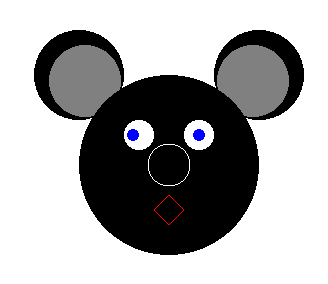
\includegraphics[width=0.4\linewidth]{images/circle_exercise.png}
\caption[]{Pay attention to the eyes!}
\label{fig:pos2D}
\end{figure}

\section{Edge2}
An \eeClass{Edge2} is a line. Just as with \eeClass{Vec2}, the '2' is important. The code will still be valid when you use an \eeClass{Edge} instead of an \eeClass{Edge2}, but that class is intended for drawing in 3D instead. To define an \eeClass{Edge2}, you need two points (\eeClass{Vec2}), being the beginning and the end. Esenthel offers two methods to pass these to the object:

\begin{code}
Edge2 e1;
Edge2 e2;

// using newly created vectors ...
e1.set(Vec2(0, 0), Vec2(0.1, 0.1));

// ... or existing vectors
Vec2 pos1(0.3, 0.6);
Vec2 pos2(0.1, 0.2);
e1.set(pos1, pos2);

// set all x and y values as floats
e2.set(-0.4, 0.2, -0.7, 0.9;
\end{code}

\subsection{Methods}
An \eeClass{Edge2} provides several neat methods. The most obvious will be \eeFunc{draw()}:

\begin{code}
line1.draw(PURPLE    ); // draw a purple line
line2.draw(GREEN, 0.1); // draw a green line, with width 0.1
line3.draw(GREEN, RED); // draw a line that starts out green but fades to read
\end{code}

Other methods of interest are \eeFunc{center()}, \eeFunc{delta()}, \eeFunc{dir()} and \eeFunc{length()}. All of them can be found in $\Rightarrow$ Math $\Rightarrow$ Shapes $\Rightarrow$ Edge.

\subsection{Exercises}

The methods \eeFunc{Sin()} en \eeFunc{Cos()} allow you to retrieve the sine and cosine from any value. This is most fun when that value is the current time. The result over time is a value which moves smoothly between -1 and 1.

\begin{code}
float x = Sin(Time.curTime());
float y = Cos(Time.curTime());
\end{code}

\begin{enumerate}
\item The code above illustrates how to use the sine and cosine with the current time. Create an application which shows a line, starting from the middle of the screen towards the current value of sine and cosine for the x and y value of the ending.
\item Change the width of the line.
\item Make the line move at double speed.
\item Decrease the length of the line. 
\item \textit{(This will be a bit harder)} Try to create an analog watch.
\end{enumerate}

Take a look at Esenthel Engine $\Rightarrow$ Math $\Rightarrow$ Shapes $\Rightarrow$ Edge. Examine the method \eeFunc{lerp(float s)}. This function needs an argument between zero and one, and return a position on the line.

\begin{enumerate}
\item Define an \eeClass{Edge2} and a \eeClass{float} with value zero.
\item In the init function, assign a start and end position to your line.
\item In the update function you increase the float with \eeClass{Time.d()}. When the float value is larger than 1, is should be assigned 0.
\item Draw the line in black with a width of 0.05. Construct a \eeClass{Vec2} with the result of \eeFunc{lerp()}. The argument of the method should be your float. Draw this point in red, also with a width of 0.05.
\end{enumerate}

Draw a triangle on the screen.

\section{Rect}
The last shape in the chapter is a rectangle: \eeClass{Rect}. You will end up using this shape quite a lot, because a rectangle happens to be the shape of most gui elements, like buttons, windows and images.

After the last exercise, you know that you need 3 positions to draw a triangle. Logic dictates a rectangle requires 4 positions, right? But there's one property of a rectangle that makes it a lot easier: all corners have an angle of 90\%. This means that when you pass the lower left corner and the upper right corner, there is enough information to find the two remaining corner positions.

\begin{figure}[h]
\centering

\includegraphics[width=0.8\linewidth]{images/rectangle.png}
\caption[]{The corners of a rectangle}
\label{fig:rect}
\end{figure}

This means a rectangle can be created like this:

\begin{code}
Rect(Vec2(-0.2, -0.1), Vec2(0.2, 0.1)).draw(BLACK, false);
\end{code}

Again there is a draw function with the color as the first argument. And optionally you can draw only the perimeter of the rectangle. Just as with \eeClass{Edge2} there is another version of the constructor allowing you to enter the x- and y-coordinates one by one.

\begin{code}
Rect(-0.2, -0.1, 0.2, 0.1).draw(BLACK);
\end{code}

\subsection{A moving Rectangle}
If you want to draw an image on the screen, it will require a rectangle. As such, a rectangle will be the basis of almost every element on your screen. It will often come in handy to have a special class for movable rectangles. As an example, we'll create a rectangle which can be moved with the arrow keys.

Rectangles have one big disadvantage when you try to move them. Instead of a central position, both corners have to be moved. This is why we often use a \eeClass{Vec2} to remember the center position. As an extra, this class will remember its color.


\begin{code}
class movableRect {
  	Vec2 pos;
	Color color;
}
\end{code}

This class can be extended with a create, update and draw methods. The create method can be used to pass the color and the starting position to the object. This starting position already has a default value, so you can use the create method without it.

\begin{code}
void create(C Color & color, C Vec2 & pos = 0) {
  	T.color = color;
	T.pos = pos;
}
\end{code}

\begin{note}
There some other new stuff in this method. The \& sign indicates that the color and pos will be passed as a reference. The character \eeFunc{C} means we will not change the value that was passed into the method. You will learn more about this in one of the next chapters. Within the function, the character \eeFunc{T} is used to solve a practical problem. The class and the method both have a variable named `color'. This makes it impossible for the compiler to know what variable you mean. You could rename one of them, but that makes the code harder to read. A more elegant solution is to add \eeFunc{T.} before the class variable. T stands for `this' and by that we mean `this class'. The version without \eeFunc{T.} will be the local variable, passed into the method.
\end{note}

Within the update method, the position can be changed by using the arrow-keys. You came across this code before, in chapter \ref{chapter:keyboardInteractie}.

\begin{code}
void update() {
	if(Kb.b(KB_LEFT )) pos.x -= Time.d();
	if(Kb.b(KB_RIGHT)) pos.x += Time.d();
	if(Kb.b(KB_UP   )) pos.y += Time.d();
	if(Kb.b(KB_DOWN )) pos.y -= Time.d();
}
\end{code}

The final thing we need is a draw function. Notice that this is the only place we actually create a rectangle. That's because we don't really need the whole rectangle in the other methods. This could be different if, for example, we need to check if the rectangle hits another object. So you could add a real \eeClass{Rect} to this class, but right now it is not needed.

\begin{code}
void draw() {
  Rect(pos - Vec2(0.2, 0.1), pos + Vec2(0.2, 0.1)).draw(color);
}
\end{code}

As you see, we use the position `pos' when we create the rectangle. The position will be the middle of the rectangle. But we still need to define the corner. This can be done be subtracting and adding the same value from the position. In this case the value is literal, but a more advanced class could just define a \eeClass{Vec2 size} and use that instead. That would make it easy to define movable rectangles of different sizes.

The whole class is listed again below. It is the first time in this course we actually create a new class, so be sure you understand what is going on. And pay attention to the keywords \eeClass{private} and \eeClass{public}. You should know those from an introductory c++ course. We will talk more about those later on, but remember they are part of a good programming style.

\begin{code}
class movableRect {
private:
  Vec2 pos, size;
	Color color;
	
public:
  void create(C Color & color, C Vec2 & pos = 0, C Vec2 & size = Vec2(0.1, 0.1)) {
	  T.color = color;
		T.pos   = pos  ;
		T.size  = size ;
	}
	
	void update() {
		if(Kb.b(KB_LEFT )) pos.x -= Time.d();
		if(Kb.b(KB_RIGHT)) pos.x += Time.d();
		if(Kb.b(KB_UP   )) pos.y += Time.d();
		if(Kb.b(KB_DOWN )) pos.y -= Time.d();
	}
	
	void draw() {
		Rect(pos - size, pos + size).draw(color);
	}
}
\end{code}
	
\subsection{Exercises}

\begin{enumerate}
\item Recreate this screen in an application:

\begin{figure}[h]
\centering
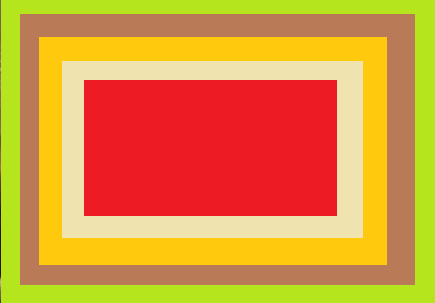
\includegraphics[width=0.4\linewidth]{images/nested_rectangles.png}
\caption[]{Rectangles}
\label{fig:nested_rect}
\end{figure}

\item Add a pink square to the application, using the newly created class \eeClass{movableRect}.
\item \textit{(A bit harder)} Be sure the square cannot move outside of the screen.
\end{enumerate}

\section{Cuts}

A function that is used very often in combination with shapes is \eeFunc{Cuts}. There are quite a lot of different versions of this function, but its meaning is always the same: do two shapes overlap, or don't they? The \eeFunc{Cuts} function allows you to check if a dot is inside a circle, if a circle (partially) overlaps a rectangle, if a line cuts a rectangle and so on. 

To check if a dot is inside a circle, use the code below:

\begin{code}
Vec2 pos(0.1, 0.1);
Circle area(0.3, Vec2(0));

if(Cuts(pos, area)) area.draw(RED);
\end{code}

Of course, in this example it is already certain the dot will always be inside the circle. But you could use the same principle to see if the mouse pointer is inside the circle, like this:

\begin{code}
Circle area(0.1, Vec2(0));

if(Cuts(Ms.pos(), area)) area.draw(RED);
else area.draw(BLACK);
\end{code}

The code above is the starting point for many possible interactions. Often, this will be in combination with other rules. Try to find out what the code below does:

\begin{code}
Rect button(Vec2(-0.2, -0.1), Vec2(0.2, 0.1));
bool hover = false;

// in the update function:
if (Cuts(Ms.pos(), button)) {
    hover = true;
	if(Ms.bp(0)) exit();
} else hover = false;

// in the draw function:
if(hover) {
  button.draw(Color(0, 255, 0));
} else {
  button.draw(Color(0, 155, 0));
}
\end{code}

\begin{exercise}
\begin{enumerate}
\item Create an application with 3 circles, each one below the other. Only the border of the circles is drawn, unless the mouse pointer is in that particular circle. In which case you draw a filled circle.
\item Make the circles move slowly to the right as long as the mouse pointer is inside the circle.
\item Create an integer `score'. When the circle goes over the right side of the screen, increase the score by one and place the circle back in the middle.
\end{enumerate}

\textit{(A bit harder) } Create your own class that behaves like a button, with a hover effect. The button also needs a line of text, which will be set by the create function.
\end{exercise}




\chapter{Images and Sound}
\section{Images}
A modern 2D game will almost always contain images. Whatever happens on the screen, it mostly comes down to showing and manipulating images. And because every image is a rectangle, you will use the \eeClass{Rect} class to show them on the screen.

\begin{code}
Images(=== drop image here ===).draw(Rect(-0.1, -0.1, 0.1, 0.1));
\end{code}

You can use \eeClass{Images()} to refer to any image in your project. The image in question can be dropped as the function argument, between the parentheses. Once that is done, you use the function \eeFunc{draw} with a \eeClass{Rect} argument to show the image on the screen. It is very easy to make your image move this way. The only thing your application has to remember is the current position. The actual rectangle can be derived from that point.

\begin{code}
Vec2 ship(0, -0.8);

// during update:
if(Kb.b(KB_LEFT )) ship.x -= Time.d();
if(Kb.b(KB_RIGHT)) ship.x += Time.d();

// during draw:
Images(=== spaceship ===).draw(Rect(ship - 0.1,  ship + 0.1));
\end{code}

\begin{note}
When you're looking for images like the one in this example, just use google images. Mostly you will want images with a transparent background. This will be an image in GIF or PNG format. But Esenthel doesn't support GIF, so PNG is your target of choice. The search tools on Google Images allow you to search specifically for transparent images. Can't find what you're looking for? Try adding the term `icon' or `sprites' to your query.

Just remember this is great while you're experimenting. But once you're working on a real game you should not use images which aren't yours, unless you really verified their license permits the use you intend.
\end{note}

To add realism to your game it is a good idea to use variations on an image. In the next example, two alternate versions of the same image are used during movement.

\begin{code}
if(Kb.b(KB_LEFT))
{
	Images(=== spaceship ===      ).draw(Rect(ship - 0.1,  ship + 0.1));
} else if(Kb.b(KB_RIGHT))
{
	Images(=== spaceship_left === ).draw(Rect(ship - 0.1,  ship + 0.1));
} else
{
	Images(=== spaceship_right ===).draw(Rect(ship - 0.1,  ship + 0.1));
}
\end{code}

\begin{exercise}
Find 3 very sad images and create an application with a moving image. Make sure the images are switched one way or another.
\end{exercise}

Another way to add some dimension is by varying the image over time. You actually create a little animation by rotating through a list of images all the time. The following example presents a player class with three variations for every direction.

\begin{code}
class player
{
private: 
   Vec2 pos;
   float timer = 0.4; 
   DIR_ENUM dir = DIRE_DOWN;
   
public:    
   void update()
   {
      // adjust direction
      if(Kb.bp(KB_UP   )) dir = DIRE_UP   ;
      if(Kb.bp(KB_DOWN )) dir = DIRE_DOWN ;
      if(Kb.bp(KB_LEFT )) dir = DIRE_LEFT ;
      if(Kb.bp(KB_RIGHT)) dir = DIRE_RIGHT;
      
      // update position
      switch(dir)
      {
         case DIRE_UP   : pos.y += Time.d() * 0.5; break;
         case DIRE_DOWN : pos.y -= Time.d() * 0.5; break;
         case DIRE_LEFT : pos.x -= Time.d() * 0.5; break;
         case DIRE_RIGHT: pos.x += Time.d() * 0.5; break;
      }
      
      // animation timer
      timer -= Time.d();
      if(timer < 0) timer = 0.4;
   }
   
   void draw()
   {
      // pointer to an image
      ImagePtr current;
      
      // evaluate direction
      switch(dir)
      {
         case DIRE_UP:
         {
            // pick an image according to time (changes between 1 - 2 - 3 - 2)
            if      (timer > 0.3) current = Images(=== back1 ===);
            else if (timer > 0.2) current = Images(=== back2 ===);
            else if (timer > 0.1) current = Images(=== back3 ===);
            else                  current = Images(=== back2 ===);
            break;
         }
         
         case DIRE_DOWN:
         {
            if      (timer > 0.3) current = Images(=== front1 ===);
            else if (timer > 0.2) current = Images(=== front2 ===);
            else if (timer > 0.1) current = Images(=== front3 ===);
            else                  current = Images(=== front2 ===);
            break;
         }
         
         case DIRE_LEFT:
         {
            if      (timer > 0.3) current = Images(=== left1 ===);
            else if (timer > 0.2) current = Images(=== left2 ===);
            else if (timer > 0.1) current = Images(=== left3 ===);
            else                  current = Images(=== left2 ===);
            break;
         }
         
         case DIRE_RIGHT:
         {
            if      (timer > 0.3) current = Images(=== right1 ===);
            else if (timer > 0.2) current = Images(=== right2 ===);
            else if (timer > 0.1) current = Images(=== right3 ===);
            else                  current = Images(=== right2 ===);
            break;
         }
      }
      
      // show the current image on the screen
      current->draw(Rect(pos - 0.05, pos + 0.05));
   }   
}
\end{code}

\begin{exercise}
The example above can be found in the course template. Create an object of the player class and use it in an application to see the result of this code.
\end{exercise}

\begin{note}
On line 39 there's an object `current' of the class \eeClass{ImagePtr}. this class is a `pointer' to an \eeClass{Image}. The code below that line will make the pointer `point' to the image we want to show next. At the bottom, \verb|current->draw()| is used to draw that image. Note the arrow instead of the dot. This is a sign that current is not a real image object, but just points to one. (Don't worry if you find this hard to grasp. You will learn more about pointers in another chapter.)
\end{note}

\begin{exercise}
The \eeClass{Image} class in Esenthel contains a whole bunch of functions. Most of them you will not need any time soon, but it is good to remember that whatever you want to do with your image, there's a good chance there is a function which has you covered.

For now, experiment a bit with the functions below to learn about their intent.

\begin{itemize}
\item \eeFunc{draw} has a version which allows you to pass some colors as an argument. Try this out. (Hint: the second color will very often be \eeFunc{TRANSPARENT})
\item Draw an image using \eeFunc{drawFit}. How does this differ from \eeFunc{draw}?
\item Draw an image using \eeFunc{drawRotate}. Try rotating the image with the arrow keys.
\item Draw an image using \eeFunc{drawFS}
\item (a bit harder) Load an image, apply a blur and export as PNG. Can you do it?
\end{itemize}
\end{exercise}

\section{Sound}
To make your game a bit more attractive you will want to add sound. Generally speaking, there are two groups: music and effects (FX). Music will mostly be played in the background while FX is linked to certain actions like pressing a button or dying horribly.

\subsection{Music}
A soundtrack can be played with the class \eeClass{Sound}:

\begin{code}
Sound soundtrack;

void InitPre()
{
   EE_INIT();
}

bool Init()
{
   soundtrack.create(=== drop your audio file here ===);
   return true;
}

void Shut() {}

bool Update()
{
   if(Kb.bp(KB_ESC)) return false;
   
   if(Kb.bp(KB_SPACE))
   {
      if(soundtrack.playing())
      {
         soundtrack.pause();
      } else
      {
         soundtrack.play();
      }
   }
   return true;
}
\end{code}

There's a few things to remember, though:

\begin{itemize}
\item Before you can use a sound, it must be loaded from disk. This is done with the \eeFunc{create()} function. It needs at least one argument: the audio file. Like with images, you can simply drag the file from your resources on to your function. You will want to do this inside of the \eeFunc{Init()} function, because you don't want to load your file from disk at every update.
\item \eeFunc{play()} will cause the sound to start playing.
\item \eeFunc{pause()} will pause the sound. Who would have guessed, right? When you use play after pause, the sound will continue right where it left off. 
\item Instead of \eeFunc{pause()} you can also use \eeFunc{stop()}. Now when you start playing again, the sound will start from the beginning.
\end{itemize}

The \eeFunc{create()} function also has a few optional arguments. Here's an example with all of them:

\begin{code}
soundtrack.create(=== audio file ===, true, 0.8, VOLUME_MUSIC);
\end{code}

But what do they mean, little grasshopper?

\begin{enumerate}
\item The first argument is known. That's the audio file.
\item the second argument is the loop value. It can be true or false and is used to indicate if you'd like the sound to `loop'. (Which mean it will start from the top when it is finished.) The default value is false.
\item Next comes the volume. Volume scales from zero to one, with a default of 1.
\item The last argument is a `channel'. Esenthel has several channels for playing audio. If you don't use this argument, the sound will use the channel `VOLUME\_FX'. It is generally a good idea to use several channels for different types of sounds, because the volume of a channel can be changed. It makes it easy to implement volume changes for music, fx or voices.
\end{enumerate}

\begin{exercise}
Create an application which loads a soundtrack. Draw a green, an orange and a red circle on the screen. The track should start playing when you click the green circle, pause when you click the orange circle and stop when you click the red one.
\end{exercise}

\begin{exercise}
\textbf{Extra:} Search the header file of the sound class for a method to retrieve the current playing position within a sound file. Draw this position on the screen. 
\end{exercise}

\begin{exercise}
\textbf{Extra:} This will be a bit harder. Use the functions \eeFunc{fadeInFromSilence()} and \eeFunc{fadeOut()} to apply a fade of 3 seconds instead of an immediate start and stop.
\end{exercise}

\subsection{Playlists (Extra)}
To play music, you can also use playlists. This will bring more variation to your soundtrack, and also allows you to switch between playlists when the mood of the game changes. Just examine the code below to see how it works:

\begin{code}
// defined play lists
Playlist Battle , // battle playlist 
         Explore, // exploring playlist
         Calm   ; // calm playlist

void InitPre()
{
   EE_INIT();
}

bool Init()
{
   if(!Battle.songs()) // create 'Battle' playlist if not yet created
   {
      Battle += (=== drop action music ===); // add "battle0" 
      Battle += (=== same here ===); // add "battle1" 
   }
   if(!Explore.songs()) // create 'Explore' playlist if not yet created
   {
      Explore+= (=== drop tranquil music ===); // add "explore" track 
   }
   if(!Calm.songs())  // create 'Calm' playlist if not yet created
   {
      Calm   += (=== a very relaxed soundtrack ===); // add "calm" 
   }
   return true;
}

void Shut()
{
}

bool Update()
{
   if(Kb.bp(KB_ESC))return false;
   if(Kb.c('1'))Music.play(Battle );
   if(Kb.c('2'))Music.play(Explore);
   if(Kb.c('3'))Music.play(Calm   );
   if(Kb.c('4'))Music.play(null   );
   return true;
}

void Draw()
{
   D.clear(TURQ);

   if(Music.playlist()) // if any playlist playing
   {
      D.text(0, 0, S+"time " +Music.time()+" / "+Music.length()+" length");
   }else
   {
      D.text(0, 0, "No playlist playing");
   }
   D.text(0, -0.2, "Press 1-battle, 2-explore, 3-calm, 4-none");
}
\end{code}

\subsection{FX}
Short sounds can also be played with the method \eeFunc{SoundPlay()}. This will play the sound directly, without requiring you to create an object of the class \eeClass{Sound}. Because there is no object you won't have any control over the sound after you started it. Therefore this technique will mostly be used for very short effects, such as footsteps. 

\begin{exercise}
In the template project you will find a few sounds in the folder `sound'. Create an application that plays back a `blip' every time you push the arrow-down key. Use the `rotate' sound for arrow-left and arrow-right. And last, play back the `down' sample when you press the space bar.

\textbf{Extra:} Add the soundtrack again, but this time control the volume of the track with the mouse wheel.
\end{exercise}
 

\part{Basics}
\chapter{Random}

\section{Whole Numbers}
A game will rarely stay interesting when it is completely predictable. To avoid predictability, developers use random values provided by the \eeClass{Random} class. The function \eeFunc{Random()} returns a random number between 0 and 4.294.967.295. Check this yourself with the next example:

\begin{code}
uint number = 0;

bool Update() {
  if(Kb.bp(KB_SPACE)) number = Random();
	return true;
}

void Draw() {
	D.clear(BLACK);
	D.text(0, 0, S + number);
}
\end{code}

You will rarely need a number this big. Which is why you can use the \eeClass{Random()} function with one or more arguments. When used with one argument, the function will return a number in the range 0 to the argument minus one. In other words, \eeClass{Random(5)}  will return one of the values 0, 1, 2, 3 or 4. Count them, that's 5 different values. A common beginners mistake is to expect the number five as a result. That will never, ever happen!

It is also possible to pass two arguments. \eeClass{Random(-2, 4)} returns one of these values: -2, -1, 0, 1, 2, 3 of 4. The important thing to remember that with this version, the arguments are inclusive.

\begin{exercise}
Create the basics of a lottery application. Show a new number from 1 to 42 (inclusive) on the screen every time you press the space bar. 
\end{exercise}

\begin{note}
How to get a random color? The RGB values which make up a color have a value between 0 and 255. To randomize a color, try this:

\begin{code}
Color myColor;
myColor.set(Random(255), Random(255), Random(255));
\end{code}
\end{note}

\section{Random Float}
So far we've discussed random whole numbers. But you will often need floating point values. These are provided by the function \eeFunc{RandomF()}. This function will return a value between 0 and 1 by default, but it will also accept arguments. \eeFunc{RandomF(3)} will return a value between 0 and 3. \eeFunc{RandomF(-1.3, 2.5)} returns one between -1.3 and 2.5.

These functions are often used to show an object on a random position. Like so:

\begin{code}
Circle c;

c.pos.x = RandomF(-D.w(), D.w());
c.pos.y = RandomF(-D.h(), D.h());
\end{code}

In the example above, we won't even pass actual numbers to the function \eeFunc{RandomF()}. Instead, we let our application decide. The width and height of the screen are not the same on every device. By asking the engine about it, we will always end up with the correct values.

\begin{exercise}
\begin{enumerate}
\item Create an application which shows a circle on the screen. Every time the space bar is pressed, you change the circle's position.
\item Create an application with a small rectangle on the screen. Assign a new position every second. 
\item Starting from the previous exercise, add an int `score' equal to zero. Draw this score somewhere on the screen. When the left mouse button is pressed, check if the mouse pointer is on top of the rectangle. If it is, increase the score by one.
\item \textit{(A bit harder)} With every score increase, the position of the rectangle should change a bit faster.
\end{enumerate}  
\end{exercise}




\chapter{Containers}

So far, you needed to define all global objects at the head of your application file. This is no problem for a little exercise, but when your project grows in size, this becomes a problem. You also have to know upfront how many objects you need. Even for a little game like asteroids, it is impossible to know how many rocks there will be on the screen at all times.

When you need several objects of the same type, you can use a container. When you declare a container for a certain object type, you can add objects to this container during the course of the application. An easy to use container is \eeClass{Memx}. The declaration of a container requires that you provide the type of objects it will contain. When you need a container for floats, you would declare it as a \eeClass{Memx<float>}. A container for rectangles would be a \eeClass{Memx<Rect>}. Look at this code for an example of a container with circles:

\begin{code}
// Declare a container for circles
Memx<Circle> circles;

void InitPre()
{
   EE_INIT();
}

bool Init()
{
    // add 10 circles to this container  
	for(int i = 0; i < 10; i++)
    {
	    // The method New() adds a new circle to the container. 
	    // At the same time the Circle method set() is used to 
	    // assign a radius and a position.
        circles.New().set(0.1, RandomF(-D.w(), D.w()), RandomF(-D.h(), D.h()));
   }
   return true;
}

void Shut() {}

bool Update()
{
   if(Kb.bp(KB_ESC)) return false;  
   return true;
}

void Draw()
{
   D.clear(BLACK);
   
   // Go over all circles in the container and
   // draw them on the screen.
   for(int i = 0; i < circles.elms(); i++)
   {
      circles[i].draw(RED);
   }
}
\end{code}

\begin{exercise}
\begin{enumerate}
\item What would happen if, by mistake, you place the code to generate circles in Update instead of Init?
\item Put this code back in Init, but add code to the Update function: every time you press the space bar, an extra circle should be added to the container.
\item Show an image on the screen instead of a circle. \textit{(Too hard? Start with a rectangle!)}
\end{enumerate}
\end{exercise}

\section{New()}
The method \eeFunc{New()} creates a new element at the end of the container. At the same time, it returns a reference to this new element, which is why can use the \eeClass{set()} method of circle in the example above. 

But suppose you need to use two methods of the newly created object? You could try something like this:

\begin{code}
for(int i = 0; i < 10; i++)
{
	circles.New().set(0.1, RandomF(-D.w(), D.w()), RandomF(-D.h(), D.h()));
	circels.New().extend(-0.05);
}
\end{code}

\ldots but it won't work. Instead you are creating two new circles at every iteration. The method \eeFunc{set} is called on the first circle, the method \eeFunc{extend} at the second. The solution is simple: Pass the result of \eeFunc{New()} to a temporary variable. The type of this variable must be a reference to a circle. (If you don't know what a reference is, don't worry. We'll talk about it later. For now, remember that you need to put an ampersand (\&) between the type and the name.

\begin{code}
for(int i = 0; i < 10; i++)
{
	Circle & c = circles.New();
	c.set(0.1, RandomF(-D.w(), D.w()), RandomF(-D.h(), D.h()));
	c.extend(-0.05);
}
\end{code}

\section{Using objects}
Very often, you need to iterate over all elements in a container. For example when you draw them all on the screen. It would be very annoying if you had to remember somehow exactly how many elements a container contains. Fortunately, you do not have to. Containers provide a method \eeFunc{elms()} which returns the current number of elements. And to access individual elements you can use square brackets, just like with primitive C arrays.

\begin{code}
for(int i = 0; i < circles.elms(); i++)
{
  circles[i].draw(RED);
}
\end{code}

Because you will need an iteration like this very, very often, Esenthel provides a `shortcut'. A macro \eeFunc{REPA} exists to replace the whole for-loop declaration with one instruction:

\begin{code}
REPA(circles)
{
  circles[i].draw(RED);
}
\end{code}

Remember this as `repeat all'. \textit{(Or don't remember it at all. Plain for-loops will always work just as well.)} And you can do more with this than just draw every element on the screen. Take a look at the next example and try to figure out what it does.

\begin{code}
REPA(circles)
{
	circles[i].pos.y += Time.d();
	if(circles[i].pos.y > D.h()) {
	  circles[i].pos.y -= (2*D.h() + RandomF(1));
	}
}
\end{code}

\begin{exercise}
\begin{enumerate}
\item Test the code above in an application. What function would you place this code in?
\item Add a function to add an extra circle every time you hit the space bar.
\item Instead of a fixed radius, use a random value between 0.01 and 0.1.
\item Draw only the perimeter of the circle, in white, on a blue background.
\item If there are any people nearby, shout out loud what this looks like.
\end{enumerate}
\end{exercise}

\section{Adding Objects}
You will add objects to a container quite a lot. This might happen in the Init function as well as the Update function. Below are a few examples to get you started, but there are a lot of different ways to add objects. It is up to you to figure out what is the best approach in your application.

\subsection{During Init}

Ten circles on random positions:

\begin{code}
for(int i = 0; i < 10; i++)
{
	Circle & c = circles.New();
	c.set(0.1, RandomF(-D.w(), D.w()), RandomF(-D.h(), D.h()));
}
\end{code}

Circles from the left to the right side of the screen:

\begin{code}
for(float i = -D.w(); i < D.w(); i += 0.2) {
  circles.New().set(0.1, i, 0);
}
\end{code}

Squares placed evenly over the screen:
\begin{code}
for(float i = -D.w(); i < D.w(); i += 0.2)
{
	for(float j = -D.h();  j < D.h();  j += 0.2)
	{
		 rects.New().set(i - 0.05, j - 0.05, i + 0.05, j + 0.05);
	}     
}
\end{code}

\subsection{During Update}

Respond to keyboard input:
\begin{code}
if(Kb.bp(KB_SPACE)) {
  circles.New().set(RandomF(0.05, 0.2), RandomF(-D.w(), D.w()), RandomF(-D.h(), D.h()));
}
\end{code}

Use the mouse position:
\begin{code}
if(Ms.bp(0)) {
  circles.New().set(0.05, Ms.pos());
}
\end{code}

With a timer:
\begin{code}
Flt timer = 3; // put this line on to of the file. Next lines belong in Update()

if(timer > 0) timer -= Time.d();
else {
  timer = 3;
	circles.New().set(RandomF(0.05, 0.2), RandomF(-D.w(), D.w()), RandomF(-D.h(), D.h()));
}
\end{code}

\begin{exercise}
Test all of the examples above and make sure you understand every one of them. Always add code to display all elements on the screen.
\end{exercise}

\section{Removing Objects}
Of course you also want to remove objects from a container. Which is not that hard:

\begin{code}
Memc<Vec2> dots;

// ... add a lot of dots

dots.remove(0); // remove the first dot
\end{code}

With the method \eeFunc{remove} and the index of the element as an argument, you delete an object in a container. Be careful though. Very often you will want to remove an element while iterating over a container. It is a common beginner mistake to alter an object after you've deleted it:

\begin{code}
for(int i = 0; i < dots.elms(); i++) {
    if(dots[i].y < -D.h()) {
        dots.remove(i);
	}
	dots[i].y -= Time.d();
}
\end{code}

In the example above, all dots are moved down at every update. When a dot arrives at the bottom of the screen, it will be removed from the container. After removing a dot, it is not the current dot that is moved down, but the next one in the container. This is not a big problem, unless this was actually the last dot in the container. In which case you try to move down an object past the end of the container. The result will be a program crash, your computer might explode and probably a kitten will die somewhere.

To prevent this from happening it is a good rule to put the remove method as the last statement in the loop:

\begin{code}
for(int i = 0; i < dots.elms(); i++) {
	dots[i].y -= Time.d();
  if(dots[i].y < -D.h()) dots.remove(i);
}
\end{code}

Things start to be a bit more complicated when you combine more than one container. In the next example we have container for dots and a container for circles. The code tries to verify if a dot hits a circle. If this is the case, both the circle and the dot must be removed from their container. To do this, we have to check every dot against every circle.

\begin{code}
for(int i = 0; i < dots.elms(); i++) {
	for(int j = 0; j < circles.elms(); j++) {
	    if(Cuts(dots[i], circles[j])) {
		    dots.remove(i);
		    circles.remove(j);
		    // At this point there is one less dot in the container, but next circles will
		    // still be compared against the current dot. If we are at the last dot, i will
		    // no longer be valid. To prevent a crash, we add a break statement to go
		    // back to the outer for loop:
			break;
		}		
	}
}
\end{code}

Of course it is also possible to empty a container at once:

\begin{code}
dots.clear();
\end{code}

\section{A little Game}

\begin{enumerate}
\item Create a triangle on the bottom of the screen which can be moved back and forth with the arrow keys.
\item Add a container for the class \eeClass{Vec2}. Every time you press the space bar, an element should be added to this container, at the current position of the rectangle.
\item Inside the update function, you increase the y value of every element in the container. (Use \eeClass{Time.d()}!) When an element reaches the top of the screen, it should be removed from the container.
\item Draw all container elements on the screen in the \eeFunc{Draw()} function.
\item Create a second container to store circles. A new circle should be added every second, at the top of the screen.
\item Make all circles move down in the Update function.
\item Show all circles in the \eeFunc{Draw()} function.
\item When a circle and a dot collide, they should both be removed.
\item When a circle collides with the triangle, show the text 'Game Over' in the middle of the screen.
\item When a circle is below the bottom of the screen, it should also be removed.
\end{enumerate}

This little project certainly can improved upon. You could stop creating new circles when the game is over, and disable the player actions. The speed at which circles appear could increase over time. Or you could show a score on the screen and provide a fixed number of lives. Another challenge could be to use images instead of circles and a triangle.


\input{\langPath basicClasses}
\input{\langPath functions}
\input{\langPath classes}
\chapter{referenties}
\label{chapter:references}

Bekijk even de volgende code:

\begin{code}
Vec som(Vec pos1, Vec pos2) {
  return pos1 + pos2;
}

// someplace else
Vec p1(0.1, 0.3, 0.5);
Vec p2(1.9, 2.7, 0.5);

Vec p3 = som(p1, p2); 
\end{code}

Alhoewel de bovenstaande code werkt zoals je verwacht, is dit helemaal niet optimaal. Je programma moet heel wat werk verrichten om de juiste waarde voor \texttt{p3} te berekenen.

Uit de leerstof van het 5de jaar heb je (hopelijk) onthouden dat een functie niet weet wat wat er in de rest van het programma gebeurt. In dit geval betekent dat dat de functie som enkel twee waarden ontvangt, die bij mekaar optelt en het resultaat ''terugstuurt'' naar het programma. 

Maar hoe kan de functie \texttt{som() p1} en \texttt{p2} optellen als die onzichtbaar zijn voor deze functie? Het antwoord is eenvoudig: op het moment dat \texttt{som()} uitgevoerd moet worden, kopi\"{e}ert de computer de waarden van \texttt{p1} en \texttt{p2} naar \texttt{pos1} en \texttt{pos2} die bestaan in de functie.

Wat terug naar het programma gaat is de waarde na \texttt{return}. Maar ook nu weet de functie niet af van \texttt{p3}. Dus kopi\"{e}ert de computer de waarde na \texttt{return} naar \texttt{p3}.

Maar nu het slechte nieuws: al dat kopi\"{e}eren kost tijd. Hieronder zie je wat er werkelijk gebeurt tijdens het uitvoeren van de functie \texttt{som()}.

\begin{itemize}
\item kopieer \texttt{p1.x} naar \texttt{pos1.x}
\item kopieer \texttt{p1.y} naar \texttt{pos1.y}
\item kopieer \texttt{p1.z} naar \texttt{pos1.z}
\item kopieer \texttt{p2.x} naar \texttt{pos2.x}
\item kopieer \texttt{p2.y} naar \texttt{pos2.y}
\item kopieer \texttt{p2.z} naar \texttt{pos2.z}
\item reserveer geheugen voor het resultaat (we noemen dit \texttt{result})
\item tel \texttt{pos1.x} bij \texttt{pos2.x} en sla de som op in \texttt{result.x}
\item tel \texttt{pos1.y} bij \texttt{pos2.y} en sla de som op in \texttt{result.y}
\item tel \texttt{pos1.z} bij \texttt{pos2.z} en sla de som op in \texttt{result.z}
\item kopieer \texttt{result.x} naar \texttt{p3.x}
\item kopieer \texttt{result.y} naar \texttt{p3.y}
\item kopieer \texttt{result.z} naar \texttt{p3.z}
\end{itemize}

En dan gebruikt deze functie nog maar eenvoudige vectoren! Wat als de argumenten containers met 2.000 vectoren zijn? Of misschien gebruik je deze \texttt{som()} functie wel op zoveel plaatsen in je code dat ze uiteindelijk 20.000 keer per seconde gebruikt wordt!

Met andere woorden: \emph{wanneer je performante software wil maken, dan moet je in de eerste plaats vermijden dat je objecten kopi\"{e}ert wanneer dat niet nodig is.}

\section{Pass by reference}
De manier waarop we tot hiertoe waarden doorgeven naar een functie, noemen we \textbf{pass by value}. We geven letterlijk de waarde van een object door, we maken met andere woorden een \textbf{kopie} van het object (in dit geval een \texttt{Vec}).

Een andere manier waarop je waarden kan doorgeven, heet \textbf{pass by reference}. Daarmee geven we niet de waarden zelf door, maar een \textbf{referentie} (of verwijzing) naar het object dat die waarden bevat.

De code ziet er dan zo uit:
\begin{code}
Vec som(Vec & pos1, Vec & pos2) {
  return pos1 + pos2;
}

// someplace else
Vec p1(0.1, 0.3, 0.5);
Vec p2(1.9, 2.7, 0.5);

Vec p3 = som(p1, p2); 
\end{code}

Het is dus slechts de \& (ampersand) die het verschil maakt. Dat lijkt misschien niet de moeite, maar het aantal stappen dat nodig is om de functie uit te voeren, kan wel flink dalen:

\begin{itemize}
\item zet een verwijzing naar \texttt{p1} naar \texttt{pos1}
\item zet een verwijzing naar \texttt{p2} naar \texttt{pos2}
\item reserveer geheugen voor het resultaat (we noemen dit \texttt{result})
\item tel \texttt{pos1.x} bij \texttt{pos2.x} en sla de som op in \texttt{result.x}
\item tel \texttt{pos1.y} bij \texttt{pos2.y} en sla de som op in \texttt{result.y}
\item tel \texttt{pos1.z} bij \texttt{pos2.z} en sla de som op in \texttt{result.z}
\item kopieer \texttt{result.x} naar \texttt{p3.x}
\item kopieer \texttt{result.y} naar \texttt{p3.y}
\item kopieer \texttt{result.z} naar \texttt{p3.z}
\end{itemize}

Het is dus bijna altijd een goed idee om een object als referentie door te geven. Enkel bij eenvoudige variabelen, zoals \texttt{int}, \texttt{float} en \texttt{bool} heeft dit geen zin. Het de referentie zou in dat geval niet even veel of zelfs meer geheugen in beslag nemen dan de waarde.

\section{return by reference}
Ongetwijfeld word je na het lezen van de bovenstaande tekst helemaal warm vanbinnen en wil je het voorbeeld nog verder verbeteren. Immers, waarom zou je ook bij de return waarde geen ampersand gebruiken?

Dus zo:
\begin{code}
Vec & som(Vec & pos1, Vec & pos2) {
  return pos1 + pos2;
}

// someplace else
Vec p1(0.1, 0.3, 0.5);
Vec p2(1.9, 2.7, 0.5);

Vec p3 = som(p1, p2); 
\end{code}

Helaas. Dit is geen goed idee. Want \texttt{p3} is nog steeds een gewone \texttt{Vec}, geen referentie naar een \texttt{Vec}. Dus dat zou betekenen:

\begin{itemize}
\item zet een verwijzing naar \texttt{p1} naar \texttt{pos1}
\item zet een verwijzing naar \texttt{p2} naar \texttt{pos2}
\item reserveer geheugen voor het resultaat (we noemen dit \texttt{result})
\item tel \texttt{pos1.x} bij \texttt{pos2.x} en sla de som op in \texttt{result.x}
\item tel \texttt{pos1.y} bij \texttt{pos2.y} en sla de som op in \texttt{result.y}
\item tel \texttt{pos1.z} bij \texttt{pos2.z} en sla de som op in \texttt{result.z}
\item \textbf{geef een referentie naar \texttt{result} als functie resultaat}
\item kopieer \texttt{result.x} naar \texttt{p3.x}
\item kopieer \texttt{result.y} naar \texttt{p3.y}
\item kopieer \texttt{result.z} naar \texttt{p3.z}

\end{itemize}

\texttt{p3} is een \texttt{Vec}, geen referentie naar een \texttt{Vec}. Dus je moet uiteindelijk de referentie toch nog kopieeren naar \texttt{p3}. Je dacht je code sneller te maken, maar ze wordt zelfs trager. Balen dus.

Maar wacht! Waarom maken we van \texttt{p3} dan niet gewoon een referentie? Ook dat is een no-go. Het probleem is dit: result is een tijdelijk object dat enkel tijdens de uitvoering van de functie bestaat. De \texttt{Vec \& p3} zou dan na de uitvoering van de functie een verwijzing bevatten naar result, maar result bestaat niet meer op dat moment.

Dit kan dus nooit goed gaan. Gelukkig zal de compiler je waarschuwen, mocht je dit willen proberen.

Kan je dan nooit een return by reference gebruiken? Toch wel. Kijk maar eens naar het volgende voorbeeld:

\begin{code}
Memc<Vec> points;
Vec & p = points.New();
p.x = 0.1;
...
\end{code}

Waarom kan dit wel? \texttt{points} is een container voor objecten van het type \texttt{Vec}. De functie \texttt{New()} maakt een \texttt{Vec} in die container en geeft een referentie als resultaat. De \texttt{Vec} bestaat dus ook na het uitvoeren van de functie nog steeds, binnen \texttt{points}. In dit geval is \texttt{p} dus een tijdelijke naam voor die \texttt{Vec} in \texttt{points}. Zo'n referentie is heel handig, omdat je via \texttt{p} een object in de container kan wijzigen waar je anders niet bij kan.

Kan dit dan nooit fout gaan? Jawel, maar dan zoek je het zelf. Als je de referentie gebruikt nadat je het object verwijdert, dan gaat het mis:

\begin{code}
Memc<Vec> points;
Vec & p = points.New();
points.clear();
p.x = 0.1; // auch!
\end{code}

\begin{exercise}
Open opnieuw de oefening die je op het eind van hoofdstuk \ref{section:managerClass} maakte. Bekijk \'e\'en voor \'e\'en de functies de je maakte. Vervang waar mogelijk een pass by value door een pass by reference.
\end{exercise}


\chapter{Pointers}

\section{Introduction}
By know you've learned that references are pretty neat. But before references existed, there were pointers. Just like references, they are used to store a memory address. But while references are hard to use wrong, pointers allow you to abuse them in every possible way. They're the bondage lovers of programming!

For instance: a reference \textsl{has} to have a valid address when you create it. And once created, the address can never change. You can't create an empty reference and pass the address later on. Pointers on the other hand, can point to anything or nothing. And you can change the contained address as many times as you like.

In most circumstances, using a reference is a lot safer. When a function asks for reference arguments, you can just provide regular objects. It's hard to do something wrong there. But you might run into problems when you want to return a reference. Take this code for example:

\begin{code}
class players {
  Memc<Player> list;
	
  Player &  add(Vec2 & pos, Str & name) {
    Player & p = list.add();
    p.set(pos, name);
    return p;
  }	  

  Player & findByName(Str & name) {
    FREPA(list) {
      if(Equal(list[i].getName(), name) {
        return list[i];
      }
    }
  }	
}
// global object
players Players;

// somewhere in your application
Players.add(Vec2(1,1), "niceGuy");
player & friend = Players.findByName("coolGuy");
\end{code}

The \eeFunc{add()} method won't give you problems. The reference arguments will always exist when you pass the to this method. (Either they are real objects, or they are existing references. And references cannot be empty.) The result will be valid too, because we are certain a new object will be made and returned.

Now take a look at the method \eeFunc{findByName()}. This method also returns a reference to a player. As long as the player you're looking for actually exists, there isn't any problem. But what if it doesn't? From what object would you return a reference? Remember, a reference can never be referencing a non existing object. So here are your options:

\begin{itemize}
  \item create a a new player: This enables you to return a valid reference to the player with this name. But when you use a method created by someone else, this is not really the behaviour you should expect. A method to find something should not create the object it is looking for. Otherwise, how are you able to find out if something exists or not?
  \item return a reference to the first player in the list: This might sound like a good idea. At least you do return a valid reference. But what if you're actually looking for that first player? The method returns the first object in the list, but now you don't know if this is because the object does not exist, or because it is actually the first object.
\end{itemize}

None of the options you have is a good idea. What we need is a way to have our method tell us ``'Hey, I don't have the object you're looking for. Stop buggering me!''. Or something slightly more polite.

\section{Pointers to the Rescue}

A pointer \textsl{can} point to an object. But it doesn't have to. They're like references without the safeguards. Here's a little idea to familiarize you with the idea:

Suppose you have a room full of lockers. Every locker can hold exactly one item. Now you put a mobile phone in locker 1. After a while, you decide to move the phone to locker 2. But just in case someone is looking for this phone in the first locker, you leave a note in there: `hey, the mobile phone is stored in locker 2 now'.

Locker 1 now points to locker 2. In fact, we can move the phone around and put it in any locker we like. As long as we update the note in locker 1, everyone is able to get our phone with just one easy step: use the location stored in locker 1.

You might be asking yourself: why on earth don't we just put the phone itself in locker 1 all the time? And you're right. Let us make it more complicated: imagine \textsl{every} locker has a phone, except for locker 1. For reasons beyond comprehension, the company owning these lockers wants to make sure all phones are used equally. So when someone uses the first phone, the next person should use the second phone. When the last phone is used, we'll have to use the first one again.

This could get really complicated. Imagine you have to notify everyone in the building that you've made phonecall and used the phone in locker 3. And everyone would have to remember that. Won't it be a lot easier to use a simple procedure?

\begin{itemize}
  \item Look in locker 1 for a pointer to another locker.
  \item Use the locker found in locker 1.
  \item Increase the locker number (pointer) in locker 1.
\end{itemize}

When all phones are completely discharged, we could even replace the note with the locker ID with an empty note. Everyone would instantly know there's no phone available when the note is empty.

\section{Pointers 101}
\subsection{Declaring a Pointer}
This is how a pointer is declared:

\begin{code}
int * p1;
int* p2;
int *p3;
Str * textPtr;
Player * playerPtr;
\end{code}

As you see, the use of spaces does not matter very much. It is best to choose one notation and stick to it. 

\subsection{Assign an Address.}
When you declare a reference, you \textsl{have} to assign a value to it. With pointers, you don't really have to do that. But you already know that an declaring an integer without assigning it a value results in a random number. The same happens with pointers. A new pointer points to a random address in memory. This is not wrong, but it will most likely crash your application when you try to use it.

\begin{code}
int * i; // could point to anything!
\end{code}

In most cases you will want to assign an actual address. This can be done by assigning the address of an existing variable. Mind though, you'll need to assign the \textsl{address} of the variabel, not the value it contains.

In other words, this is wrong:
\begin{code}
int i = 42;
int * p = i; // tries to assign the value of i as an address in p
\end{code}

The pass the address of a variable, use and ampersand (\&). Like this:

\begin{code}
int   i = 42;
int * p = &i; // declaration and initialisation
int * p;      // declaration only
p       = &i; // assign an address
p       =  i; // auch! wrong!!! 
\end{code}    


\subsection{Changing a value through its pointer}
Rather often you will use a pointer to alter the value it is pointing to. But assigning a value to the pointer itself is wrong. So how do you that? You use an asterisk.

\begin{code}
int   i = 42;
int * p = i ; // assign the address of i to p
*p      = 43; // assign a value to i through the pointer
\end{code}

It is also possible to assign the value of another pointer, like this:

\begin{code}
*p1 = *p2;
\end{code}

\subsection{Pointer to null}
An unassigned pointer points to random memory. So how do you make an `empty' pointer, pointing to nothing? You assign a `null' address. We also call this a `null pointer'.

\begin{code}
int * p1 = null;
\end{code}

You could now rewrite the code at the beginning of this chapter. Remember, the whole problem was that we could not return a name when none was found.

\begin{code}
class players {
  Memc<Player> list;
  
  // no problem with references here
  Circle &  add(Vec2 & pos, Str & name) {
    Player & p = list.add();
    p.set(pos, name);
    return p;
  }	  

  // a pointer is used instead of a reference
  Circle * findByName(Str & name) {
    FREPA(list) {
      if(Equal(list[i].getName(), name) {
        return &list[i]; // notice the ampersand!
      }
    }
    // no player found with this name
    return null;
  }	
}
// globaal object
players Players;

// somewhere in your application
Players.add(Vec2(1,1), "niceGuy");
player * friend = Players.findByName("coolGuy");

// check if the player exists
if(friend != null) {
  Greet(friend);
}
\end{code} 

When no player is found with a certain name, a null pointer will be returned. By checking if the returned value is different from null, we make sure the \eeFunc{Greet(player * p)} function is only executed with a valid player. 

\begin{note}
Some memory containers (like Memb) will move their objects around when the container grows. When there isn't enough memory in the current container, the whole container will be moved to a new memory location. This means that pointers to members of that container become invalid. If you need pointers to stay valid, use a container like Memx. Otherwise, only create pointers local to a method.
\end{note} 

\section{All together}
When working with pointers and references, we can use both the symbols \& and *. What they mean depends on the situation. Below are all the posibilities.

Suppose these variable exist:

\begin{code}
int   j   = 43;
int & ref = j ;
int * ptr = &j;
\end{code}

We can use these symbols

\begin{myTable}{references and pointers}{l||l|l}
  & reference & pointer \\ 
\hline Declaration     &      & \lstinline|int * i;| \\ 
\hline Declaration and Initialisation & \lstinline|int & i = j;|  & \lstinline|int * i = &j;|\\ 
\hline Initialisation &  & \lstinline| i = &j;| \\
\hline\hline Assign value & \lstinline|i = 42;| & \lstinline|*i = 42;| \\
\hline Assign value from variable & \lstinline|i = j;| & \lstinline|*i = j;| \\
\hline Assign value from reference & \lstinline|i = ref;| & \lstinline|*i = ref;| \\
\hline Assign value from pointer & \lstinline|i = *ptr;| & \lstinline|*i = *ptr;| \\
\hline\hline Assign address &  & \lstinline| i = &j;| \\
\hline Assign addres from reference  &  & \lstinline| i = &ref;| \\
\hline Assign address from pointer &  & \lstinline| i = ptr;| \\ 
 
\end{myTable} 

References are a bit easier to use. But also less flexible. Sometimes you really need a pointer.

\begin{exercise}
\begin{enumerate}
  \item Create an application with 5 circles, spread out on the bottom of your screen. Create a memory container to hold these circles.
	\item When the mouse is on top of a circle, it should slowly move upwards.
	\item Create a function with a pointer to the highest circle as a result. Call this function in every update and keep the result in a pointer variable.
	\item Draw all circles on the screen. Before drawing a circle, compare its address with the address of the highest circle. When they are the same, draw the circle green, otherwise draw it red.
\end{enumerate}
\end{exercise}

	
\chapter{Enumeratie}
\section{Zo moet het niet...}
Enumeraties of enum's maken het mogelijk om getallen als tekst weer te geven. Als voorbeeld gebruiken we een class enemy. Die enemy kan een warrior, een rogue of een priest zijn, en afhankelijk daarvan moet er een andere afbeelding getoond worden. Je zou boolean's kunnen gebruiken om te onthouden class de enemy heeft:

\begin{code}
class enemy {
  bool warrior = false;
	bool rogue   = false;
	bool priest  = false;
	Rect r;
	
	void setWarrior() {
		warrior = true ;
		rogue   = false;
		priest  = false;
	}
	
	// de functies setRogue en setPriest zijn gelijkaardig
	// ...
	
	void draw() {
	  if     (warrior) Images(=== warriorImage ===).draw(r);
		else if(rogue  ) Images(=== rogueImage   ===).draw(r);
		else if(priest ) Images(=== priestImage  ===).draw(r);
	}
}
\end{code}

Alhoewel bovenstaande code werkt, is ze niet erg efficient. Nu gaat het nog maar om 3 classes, maar hoe meer mogelijkheden je hebt, hoe meer variabelen je moet aanpassen bij het selecteren van een class. Veel beter zou zijn om slechts \'e\'en variabele te gebruiken, want een enemy kan tenslotte maar 1 class hebben.

\section{Dit is niet veel beter.}
Je zou kunnen beslissen dat een warrior het cijfer 0 krijgt, een rogue het cijfer 1 en een priest het cijfer 2. Dan wordt de code al veel eenvoudiger.

\begin{code}
class enemy {
  int type = -1;
	Rect r;
	
	void setType(int type) {
		T.type = type;
	}
	
	void draw() {
		switch(type) {
			case 0: Images(=== warriorImage ===).draw(r); break;
			case 1: Images(=== rogueImage   ===).draw(r); break;
			case 2: Images(=== priestImage  ===).draw(r); break;
	  }
	}
}
\end{code}

De bovenstaande code is beter dan de eerste versie, maar het is nogal onwaarschijnlijk dat je niet vergeet welk nummer voor welke class staat. Of misschien gebruik je ergens een getal waarvoor geen class is voorzien. 

\section{Enumeration time!}
De oplossing voor dit probleem zijn enum's. Enumeraties zijn lijsten van woorden. Intern wordt het eerste woord gelijk aan 0 en krijgt elk volgend woord een hoger nummer. Je kan echter steeds die woorden gebruiken in plaats van dat nummer. 

\begin{code}
enum ENEMY_TYPE {
	ET_NONE   ,
  ET_WARRIOR,
  ET_ROGUE  ,
	ET_PRIEST , 
}

class enemy {
  ENEMY_TYPE type = ET_NONE;
	Rect r;
	
	void setType(ENEMY_TYPE type) {
		T.type = type;
	}
	
	void draw() {
		switch(type) {
			case ET_WARRIOR: Images(=== warriorImage ===).draw(r); break;
			case ET_ROGUE  : Images(=== rogueImage   ===).draw(r); break;
			case ET_PRIEST : Images(=== priestImage  ===).draw(r); break;
		}
	}
}
\end{code}

Het voordeel van deze code is dat je overal in je programma de waarden \texttt{ET\_WARRIOR} of \texttt{ET\_ROGUE} kan gebruiken. Je kan de functie setType ook geen getal meegeven van een class die niet bestaat. En bovendien zie je op elk moment duidelijk over welke vrucht je het hebt. 

De waarden van een enum schrijven we in hoofdletters. Dit is niet verplicht, maar wel een conventie. Je kan immers nooit het getal waar een enumeratie waarde voor staat, aanpassen. Iets als \texttt{ET\_WARRIOR = 3} is dus onmogelijk. Aangezien \texttt{ET\_WARRIOR} het tweede woord in de rij is, is zijn waarde steeds 1.

Het is ook niet nodig om elke waarde met \texttt{ET\_} te beginnen, maar in een groter programma is het dikwijls handig om een afkorting van de enumeratie te gebruiken. ``ENEMY\_TYPE'' wordt zo ET. Op die manier kan de autocomplete je helpen met het kiezen van een naam zodra je \texttt{ET\_} getypt hebt.

\begin{note}
Esenthel bevat ook een \textsl{enumeration editor}. Hiermee kan je grafisch de waarden van een enumeratie type ingeven. Deze waarden zijn dan bruikbaar in zowel je code als de world editor.
\end{note}


\chapter{Constants}
\section{Global Constants}
Most applications will use particular values throughout the code. Imagine an application which does a lot of calculations with circles: you will definitely use the number pi a lot. You could calculate pi every time you need it, but that's not a good idea because the outcome will be the same every time. You're making your computer do needless calculations. Instead you could declare a global variable:

\begin{code}
int pi = 3.1415926;
\end{code}

With this variable, you can use pi everywhere in your code. But mistakes happen, and what about this one:

\begin{code}
int value = 1;
// ... more code ...
if(pi = value) {
  // do something
}
\end{code}

The code above won't result in an error. But instead of comparing pi, you assign a new value to pi by mistake. Auch! This mistake is easily made, but it might take a while before you realize why every calculation with pi suddenly has the wrong outcome.

It would be much better if we could prevent such a mistake from being made. After assigning a value to pi, there is no reason why it should change. We need a way to prevent changes made to this variable. That's why most programming languages provide a way to make a variable `constant'. A constant can never changes after its declaration. And to increase readability, most programmers will always write constants in capitals.

So how do you declare a constant in C++? You precede it with the word \verb|const|. Esenthel makes it even easier by defining the capital \verb|C| as \verb|const|, just like you can write \verb|T| instead of \verb|this|. In Esenthel, you could declare PI as:

\begin{code}
C PI = 3.1415926;
\end{code}

This approach has two advantages:

\begin{enumerate}
	\item The value of PI can never be changed by mistake.
	\item If, for some crazy reason, you \textit{need} to change the value of PI, you only have to change it this one instance. \textsl{(Highly unlikely in this case, but it will happen with other constant values in your application. Imagine a constant named ATTACK\_RANGE. You probably will want to experiment with that before releasing your game.)} 
\end{enumerate}

\begin{note}
Because PI is needed in almost every game, Esenthel already declared it for you. And not only PI is defined, but also a few common calculations like PI\_2 (half of PI) and PI2 (two times PI).
\end{note}

\begin{exercise}
Write an application with the following constants: playerColor, playerSize, enemyColor and enemySize. The player is a rectangle, the enemies are circles \textit{(it is a very abstract game)}. Draw a player and some enemies on the screen using these constants. 
\end{exercise}

\section{Const Arguments}
There's another situation in which constants are used. Just look at this function:

\begin{code}
float calculateDistance(Vec2 & pos1, Vec2 & pos2);
\end{code}

Suppose you can use this function to calculate the distance between two points. In chapter \ref{chapter:references} you read that it is often faster to pass a variable by reference as opposed to passing it by value. But there's a downside on that. In principle, you could alter the values of pos1 and pos2 within this function. And if a value is passed by reference, this would also change those variables in the original location. But imagine you are working in a team and the function \eeFunc{calculateDistance} is written by someone else. If something unexpected happens in your code, you would have to double check the work of your colleague to verify the values are not changed in there. The name of the function seems to indicate there's no reason for that, but mistakes happen. A lot.

It would be better if we can now for sure the values we pass to this function will not be changed by it. That way, we can focus on our own code when there's an error. The solution is simple: we can pass these references as constants:

\begin{code}
float calculateDistance(C Vec2 & pos1, C Vec2 & pos2);
\end{code}

This is much better because:

\begin{enumerate}
	\item when creating such a function, you will get an error if you try to change pos1 or pos2;
	\item the programming which uses this function can be sure the values are not changed in there, without reading your code;
	\item you have a strong indication that values \textit{will} be changed inside a function when the reference is not declared as a constant. \textit{(It's either that, or you need to have a serious talk with your fellow developers.)}
\end{enumerate}

Let's agree that, starting right now, you will pass all function arguments as a const reference, unless you have a good reason not to. Your future colleagues will like you a lot more when you do so.

And what is a good reason not to use a constant? Look at the Esenthel \eeFunc{Clamp} function:
\begin{code}
void Clamp(Vec2 & value, C Vec2 & min, C Vec2 & max);
\end{code}

This function will change the first argument when its value is lower than the second or higher than the third. It can be used like this:

\begin{code}
Vec2 pos = Ms.pos();
Clamp(pos, Vec2(-0.4,-0.4), Vec2(0.4,0.4));
pos.draw(RED);
\end{code}

The second and third argument are constant, so the function will never change the minimum or maximum. But the first argument is the one that is meant to change. No const reference there.

\begin{exercise}
\begin{itemize}
	\item Search the Engine code for more functions with non-const references. Try to explain why these references are not constant.
	\item Write a function `ClampToScreen' which changes an argument (a Vec2) when it would be outside the screen. Test your function with a simple program. Can you use a const reference?
	\item Write a function with a string argument. The function will draw the string on the screen. Create a version with a const reference and one with a non-const reference. Test both versions with existing \eeClass{Str} variables as well as with string literals. Why won't the non-const version work with string literals? 
\end{itemize}
\end{exercise}
\chapter{Application States}
\label{chapter:application_states}

Een application state is een ``status'' van het programma. Wanneer twee delen van een programma nooit gecombineerd worden, dan kan je er twee afzonderlijke application states van maken. 

Wat veel voorkomt is bijvoorbeeld een game lobby en het eigenlijke spel. Je zal nooit de elementen van een game lobby combineren met het spel, dus kan je die volledig scheiden. Ook een login module kan een afzonderlijke application state zijn.

Elk programma heeft al een default application state. Die bestaat uit de functies \texttt{Init()}, \texttt{Shut()}, \texttt{Update()} en \texttt{Draw()}. Wanneer een state actief wordt, dan wordt \texttt{Init()} uitgevoerd. Daarna worden \texttt{Update()} en \texttt{Draw()} afwisselend uitgevoerd, totdat je het programma sluit of overgaat naar een andere state. Op dat moment wordt \texttt{Shut()} uitgevoerd.

\section{Intro}
Voor elke state maak je een afzonderlijk bestand. Bijvoorbeeld voor een intro state:

\begin{code}
bool InitIntro() {return true;}

void ShutIntro() {}

bool UpdateIntro()
{
   if(Time.stateTime()>3 || Kb.bp(KB_ESC)) {
      StateMenu.set(1.0);                    
   }
   return true;
}

void DrawIntro()
{
   D.clear(BLACK);
   D.text (0, 0, "Intro");
}

State StateIntro(UpdateIntro, DrawIntro, InitIntro, ShutIntro);
\end{code}

Je ziet dat dit veel lijkt op de standaard states in je programma. We voegen gewoon het woord Intro toe aan Init, Shut, Update en Draw. Dit houdt het overzichtelijk.

De eigenlijke state zit in de laatste regel:

\begin{code}
State StateIntro(UpdateIntro, DrawIntro, InitIntro, ShutIntro);
\end{code}

Daar geef je aan dat er een nieuwe gamestate is (\eeFunc{StateIntro}) die de typische functies voor een programma bevat. Een \eeFunc{InitPre()} functie kan je niet toelaten, die dient enkel voor de echte start van het programma.

Kijk ook even naar de constructor van \eeFunc{State}:

\begin{code}
State(Bool (*update)(), void (*draw)(), Bool (*init)()=NULL, void (*shut)()=NULL); 
\end{code}

Komt de asterisk (*) je bekend voor? Inderdaad, we hebben met pointers te maken. Pointers naar functies in dit geval. De constructor verwacht dat we aangeven waar de functies voor deze state staan. We verwijzen dus naar de functies die we net gemaakt hebben: \eeFunc{UpdateIntro()} en \eeFunc{DrawIntro()}. Je zegt eigenlijk ``zolang deze state actief is, voer je \eeFunc{UpdateIntro()} uit in plaats van de gewone \eeFunc{Update()} functie.

De volgende twee argumenten, voor de functies \eeFunc{InitIntro()} en \eeFunc{ShutIntro()} zijn optioneel. Je mag ze weglaten als er niets bijzonders moet gebeuren op dat moment.

\begin{note}
Indien een functie argument eindigt met \eeFunc{=NULL}, dan mag je het weglaten.
\end{note} 

\section{Menu}
De code hierboven bevat ook een verwijzing naar StateMenu:

\begin{code}
   if(StateActive.time()>3 || Kb.bp(KB_ESC)) {
      StateMenu.set(1.0);                    
   }
\end{code}

Met andere woorden: we wachten tot de huidige state 3 seconden actief is, of totdat de gebruiker op escape drukt. Dan zetten we een nieuwe application state actief met een crossfade van 1 seconde.

Deze nieuwe state zou er zo kunnen uitzien:
\begin{code}
bool InitMenu() {return true;}
void ShutMenu() {}

bool UpdateMenu()
{
   if(Kb.bp(KB_ESC))return false;
   if(Kb.bp(KB_ENTER))StateGame.set(0.5);
   return true;
}

void DrawMenu()
{
   D.clear(GREY);
   D.text (0,  0  , "Menu");
   D.text (0, -0.3, "Press Enter to start the game");
   D.text (0, -0.5, "Press Escape to exit");
}

State StateMenu(UpdateMenu, DrawMenu, InitMenu, ShutMenu);
\end{code}

Deze state lijkt sterk op de vorige. Maar dit maal kunnen we met Enter naar de game zelf. En dat is dan ook weer een nieuwe application state: \eeFunc{StateGame}.

\section{Game}
Deze code kan je voor \eeFunc{StateGame} gebruiken. Maak ook nu weer een afzonderlijk bestand.
\begin{code}
bool InitGame() {return true;}
void ShutGame() {}

bool UpdateGame()
{
   if(Kb.bp(KB_ESC))StateMenu.set(1.0);
   return true;
}

void DrawGame()
{
   D.clear(TURQ);
   D.text (0, 0, "Game");
}

State StateGame(UpdateGame, DrawGame, InitGame, ShutGame);
\end{code}

Door tijdens de game op escape te drukken, schakelen we terug naar \eeFunc{StateMenu}. In deze state ga je bij een echte game natuurlijk nog heel veel code moeten toevoegen.

\section{Default State}
Dan rest ons nog het starten van het programma. We hebben nu alle nodige states, maar \eeFunc{StateIntro} moet nog actief worden. Dit gebeurt door in de \eeFunc{Init()} functie van het programma dadelijk door te schakelen naar \eeFunc{StateIntro}. De functies \eeFunc{Update()} en \eeFunc{Draw()} worden in dit programma dus niet gebruikt.

\begin{code}
void InitPre()
{
   EE_INIT();
}

bool Init()
{
   StateIntro.set();
   return true;
}

void Shut() {}
bool Update() {return false;} // unused
void Draw  () {             } // unused
\end{code}

\begin{exercise}
Gebruik de code van dit hoofdstuk om een programma te maken dat wisselt tussen de voorziene application states. Elke state plaats je in een afzonderlijk bestand.
\end{exercise}


\part{Tetris}
\chapter{Inleiding}
Je hebt in de vorige hoofdstukken alles gezien om een eenvoudige 2D game te maken. Maar hoe breng je dat nu op een overzichtelijke manier samen in een groot project? Er bestaat eigenlijk niet \'e\'en antwoord daarop. Je leert dat vooral door ervaring op te doen. Wat voor de ene persoon werkt, vind de andere misschien minder goed. Toch zijn er een aantal regels die het je zeker makkelijker kunnen maken. En wanneer je in groep werkt dan zal de lead programmer meestal ook een aantal regels opleggen die iedereen moet volgen. Dat zijn niet noodzakelijk goede of slechte regels, maar ze werken zolang iedereen hetzelfde doet.

In dit deel van de cursus bouw je een project op voor een tetris kloon. Je leert om stap voor stap een project uit te werken zonder dat je het overzicht kwijt raakt.

\begin{note}
Tetris bestaat uit blokken die dan weer bestaan uit vierkanten. In deze cursus bedoelen we met een blok steeds het hele tetris figuurtje. Staat er `square' of vierkant, dan gaat het om de vierkantjes die samen een blok vormen.
\end{note}

\section{Setup}
Open eerst het project `Tetris\_start'. Daarin vind je alvast de graphics, geluiden en fonts die we gaan gebruiken. Er is ook alvast een lege app `Tetris' voorzien, maar die gaan we nog niet dadelijk gebruiken.

\begin{enumerate}
	\item Maak eerst op het hoogste niveau een Library aan. Dat doe je door rechts te klikken en `new library' te kiezen. Je geeft deze library de naam `Tetris parts'. Je Een library is een groene map. De code in een library kan je gebruiken vanuit elke applicatie binnen je project, net zoals de library `Esenthel Engine' die altijd aanwezig is.
	\item Maak ook een nieuwe applicatie (blauwe map). Die noem je `squareTester'.
	\item In de applicatie `squareTester' maak je een code bestand `main'. 
	\item In de library `Tetris parts' maak je een nieuwe folder (geel) met de naam `definitions'.
	\item Maak van `squareTester' de actieve applicatie.
\end{enumerate}
	
Je kan in het bestand `squareTester/main' de code van `Tetris/initState' overnemen. Verwijder dan wel de regel 
	
\begin{code}
D.full(true);
\end{code}

Dat maakt het makkelijker om je programma te be\"indigen wanneer er iets fout gaat.	

\section{Constants}
In het vorige hoofdstuk leerde je over constanten. Het is een goed idee om, voordat je aan de echte code begint, enkele belangrijke constanten vast te leggen. Die kan je dan overal in je code gebruiken en later eenvoudig aanpassen als dat nodig blijkt. Je begint daarom in de map `Tetris parts/definitions' met een nieuw code bestand dat je `constants'noemt.

Om later de naam van het programma eenvoudig te wijzigen, maken we alvast een constante \eeClass{Str} met de voorlopige naam.

\begin{code}
C Str APP_NAME = "Tetris";
\end{code}

De grootte van het standaard applicatie window is niet ideaal voor dit spel. Die grootte moet in pixels worden ingegeven. We declareren daar een constante \eeClass{int} voor, zodat we die later eenvoudig kunnen aanpassen.

\begin{code}
// the window size on the screen, in pixels
C int WINDOW_WIDTH  = 900;
C int WINDOW_HEIGHT = 800;
\end{code}

Tetris bestaat uit rijen en kolommen. Ook die leggen we vast:

\begin{code}
// this impacts the playing field
C int SQUARES_PER_ROW = 10;
C int ROWS            = 15;
\end{code}

Over de score kunnen we ook al iets zeggen. Er moeten een aantal levels zijn, de punten die je per lijn en per level krijgt liggen ook vast.

\begin{code}
// the score system uses these
C int POINTS_PER_LINE  =  525;
C int POINTS_PER_LEVEL = 6300;
C int NUM_LEVELS       =    5;
\end{code}

De snelheid van het spel gaat elk level omhoog. We kunnen die begrippen ook al vastleggen.

\begin{code}
// the speed will increase every level
C float INITIAL_SPEED = 1.0;
C float SPEED_CHANGE  = 0.1;
\end{code}

Als je tetris speelt, dan is er een korte periode waarin je een blok dat de onderkant van het spel bereikt nog opzij kan schuiven. Die periode leggen we ook vast.

\begin{code}
// the time a block can be slided to the side
// when it hits bottom
C float SLIDE_TIME = 0.25;
\end{code}

Dan moeten we bepalen hoe groot het speelveld is. We leggen daarom de linkeronderhoek vast, en de grootte van de rechthoek die we daarop toepassen.

\begin{code}
// the area reserved for the playing field 
C Vec2 GAMEAREA     (-0.8, -0.8);
C Vec2 GAMEAREA_SIZE( 1.0,  1.4);
\end{code}

Een nieuw blok verschijnt altijd bovenaan het scherm. Waar dat precies is, dat kunnen we afleiden uit de waarden die we al hebben: SQUARES\_PER\_ROW en ROWS. Daarnaast is er ook nog een wachtpositie, die je meestal bovenaan rechts naast het speelveld toont. Het valt je misschien op dat we hier geen \eeClass{Vec2} gebruiken, maar een \eeClass{VecI2}. Dat is een vector waar enkel gehele getallen in passen. We willen geen tetris waar blokken halverwege tussen twee posities kunnen zitten.

\begin{code}
// position for the current and next block
C VecI2 STARTPOS(SQUARES_PER_ROW / 2, ROWS - 1);
C VecI2 WAITPOS (SQUARES_PER_ROW + 4, ROWS - 3);
\end{code}

Tot slot kunnen we met de voorgaande constante ook de grootte van een vierkant berekenen. Dat heeft het voordeel dat we later de voorgaande constanten kunnen aanpassen en dat de grootte van een vierkant dan vanzelf aangepast wordt.

\begin{code}
// the size of a square
C float SQUARE_SIZE = GAMEAREA_SIZE.x / SQUARES_PER_ROW;
\end{code}

\begin{note}
Het zal natuurlijk zelden gebeuren dat je bij de start aan een project al perfect weet welke constanten je nodig zal hebben. In praktijk zal je dus meestal enkele waarden vastleggen en daarna de lijst aanvullen wanneer je merkt dat je nog constanten nodig hebt.
\end{note}

\section{Enumeraties}
Maak in de folder `Tetris parts/definitions' een nieuw code bestand `enumerations'. hierin voorzie je alvast twee enum's die je in het project nodig zal hebben. Ten eerste is er het blok type. Tetris heeft vierkante blokken, T blokken enzovoort. Een lijst kan er zo uitzien:

\begin{code}
enum BLOCK_TYPE
{
   BT_SQUARE     ,
   BT_T          ,
   BT_L          ,
   BT_BACKWARDS_L,
   BT_STRAIGHT   ,
   BT_S          ,
   BT_BACKWARDS_S,
   BT_NUM        , // number of block types used in the game
   BT_BACKGROUND , // special case, only for background
   BT_WALL       ,      
}
\end{code}

De drie laatste waarden  verdienen wat extra aandacht. De waarde `BT\_NUM' is handig omdat het nummer waar die waarde voor staat, gelijk is aan de mogelijkheden + 1. Dat maakt het eenvoudig om een random functie te gebruiken. Die is immers exclusief de hoogste waarde. Zo kunnen we later in het programma eenvoudig de volgende functie gebruiken:

\begin{code}
blockType type = Random(BT_NUM);
\end{code}

Waarom staat BT\_NUM dan niet op het eind? Wel, de laatste twee waarden zijn speciale gevallen. Het is handig voor de afwerking van het spel om ook vierkanten te gebruiken om de achtergrond en de randen van het spel te tekenen. En de kleur van zo'n vierkant wordt bepaald door het blok type. Omdat we niet willen dat die types ook in het spel gebruiken, plaatsen we BT\_NUM daar voor.

Een tweede enumeratie hebben we nodig om de mogelijke richtingen van een blok te bepalen. Een blok kan nooit naar boven, maar wel naar links, naar rechts, of naar beneden. Blokken die al beneden zijn, hebben geen richting meer.

\begin{code}
enum DIRECTION
{
   D_LEFT ,
   D_RIGHT,
   D_DOWN ,
   D_NONE ,
}
\end{code}

\chapter{Objecten}
In tetris denk je vooral aan blokken. Dat die blokken uit vierkanten bestaan is voor de speler bijkomstig, maar wel belangrijk voor de ontwikkelaar. Elk vierkant kan immers een ander vierkant raken. En wanneer een blok de bodem bereikt, dan wordt het een deel van een hoop vierkanten, die rij per rij verwijderd kunnen worden, ongeacht de vorm van het oorspronkelijke blok.

\section{Squares}
Maak in de library `tetris parts' een nieuwe folder met de naam `objects'. Daarin plaats je een code bestand `square'. We maken in dat bestand een class \eeClass{square} waarin we een vierkant beschrijven.

Een vierkant moet een positie hebben. Omdat het speelveld in tetris een raster is (we kunnen een vierkant niet eender waar plaatsen!) gebruiken we opnieuw een \eeClass{VecI2} waarin we dus enkel gehele getallen kunnen opslaan. Verder moet het vierkant een \eeClass{blockType} hebben om te bepalen in welke kleur het getekend moet worden. In het bestand `enumerations' hebben we de types al vastgelegd, dus we kunnen die hier gebruiken.

De class \eeClass{square} zal ook functies nodig hebben. We voorzien een \eeFunc{create} functie om de positie en het type van het blok in te stellen. Daarnaast hebben we een \eeFunc{move} functie nodig om het blok in een bepaalde richting te bewegen. (Die richting is dan weer de tweede enum die we maakten.) We hebben ook een functie nodig om de huidige positie op te vragen en een functie om de positie rechtstreeks te veranderen. En tot slot willen we een functie om het vierkant op het scherm te tekenen.

De class ziet er dan zo uit:

\begin{code}
class square
{
private:
   VecI2      pos ; 
   BLOCK_TYPE type;
   
public:
   void create (C VecI2 & pos, BLOCK_TYPE type) { }
   void move   (DIRECTION dir)   { }
   VecI2 getPos(             ) C { }
   void setPos (C VecI2 & pos)   { }
	 void draw   (             ) C { }
}
\end{code}

Voeg de bovenstaande code alvast toe aan je project. 

\subsection{Square Tester}
Je verwacht nu waarschijnlijk dat we de inhoud van deze functies gaan toevoegen. In plaats daarvan gaan we eerst naar de applicatie `squareTester'. Je weet dat je tijdens de ontwikkeling van een programma je code heel regelmatig moet testen. Maar in een groot project is dat moeilijk. We moeten nog heel wat classes schrijven alvorens je de applicatie zou kunnen uitvoeren.

Daarom gebruiken we testprogramma's. Die schrijven we zo dat ze een specifieke class kunnen testen. In dit geval zorgen we er voor dat alle funties van de class \eeClass{square} getest kunnen worden. De code voor `squareTester' kan er bijvoorbeeld zo uitzien:

\begin{code}

Memc<square> squares;

void InitPre()
{
   EE_INIT();
}                
       
bool Init()
{   
	 // hier test je de create functie, met verschillende
	 // soorten blokken.
   squares.New().create(VecI2( 2,  2), BT_S          );
   squares.New().create(VecI2( 4,  2), BT_T          );
   squares.New().create(VecI2( 6,  7), BT_L          );
   squares.New().create(VecI2(10, 12), BT_BACKWARDS_S);
   squares.New().create(VecI2( 8,  8), BT_BACKWARDS_L);
   squares.New().create(VecI2( 5,  1), BT_SQUARE     );
	 return true;
}

void Shut() {}

bool Update()
{
   if(Kb.bp(KB_ESC)) return false;
   
	 // we declareren een richting en controleren de pijltjestoetsen
   DIRECTION d = D_NONE;
   if(Kb.bp(KB_DOWN )) d = D_DOWN ;
   if(Kb.bp(KB_LEFT )) d = D_LEFT ;
   if(Kb.bp(KB_RIGHT)) d = D_RIGHT;
   
	 // vervolgens verplaatsen we alle blokken in deze richting. Wanneer
	 // er geen toets ingedrukt werd, zouden de squares niet mogen bewegen.
   REPA(squares)
   {
      squares[i].move(d);
   }
   
	 // De functies getPos en setPos moeten ook getest worden. Dat doen we
	 // wanneer de spatiebalk ingedrukt werd. We vragen dan de huidige positie
	 // van elk vierkant en wijzigen de vertikale waarde. De gewijzigde positie wordt
	 // terug in het vierkant geplaatst.
   if(Kb.bp(KB_SPACE))
   {
      REPA(squares)
      {
         VecI2 pos = squares[i].getPos();
         pos.y += 4;
         squares[i].setPos(pos);
      }
   }
   
   return true;
}

void Draw()
{
   D.clear(BLACK);
	
	 // hier testen we de draw functie van elke square.
   REPA(squares)
   {
      squares[i].draw();
   }
}

\end{code}

\begin{note}
Je hebt dikwijls veel mogelijkheden om een testprogramma te schrijven. Het belangrijkste is dat je op een zo eenvoudig mogelijke manier zoveel mogelijk functies van je class kan testen. Zo voorkom je dat er later fouten opduiken wanneer je alle classes samenvoegt.
\end{note}

\subsection{Create en Draw}
De create functie van square is heel eenvoudig. Je moet er voor zorgen dat de argumenten in de variabelen van de class terecht komen. Werk die functie nu zelf uit.

Iets moeilijker is de draw functie. Daarom overlopen we eerst even wat deze functie moet kunnen.

\begin{enumerate}
  \item Afhankelijk van het BLOCK\_TYPE moet de kleur gekozen worden. 
	\item De positie van de square is de positie in de grid. We moeten de werkelijke positie op het scherm berekenen.
	\item We moeten een afbeelding op het scherm tonen.
\end{enumerate}

De kleur bepalen doen we via een switch statement. We declaren een variabele van het type \eeClass{Color} en de waarde BLACK. Daarna wijzigen we dit in de gewenste kleur voor elk type:

\begin{code}
Color color(BLACK);
      
switch(type)
{

case BT_SQUARE     : color = RED   ; break;
	 case BT_T          : color = PURPLE; break;
	 case BT_L          : color = GREY  ; break;
	 case BT_BACKWARDS_L: color = BLUE  ; break;
	 case BT_STRAIGHT   : color = GREEN ; break;
	 case BT_S          : color = PINK  ; break;
	 case BT_BACKWARDS_S: color = YELLOW; break;
	 case BT_BACKGROUND : color = Color(50, 50, 50) ; break;
	 case BT_WALL       : color = WHITE ; break;
}
\end{code}

Dan moeten we de positie bepalen. In de constante GAMEAREA staat de linkeronderhoek van het speelveld. Alle posities worden vanuit dat punt berekend. De linkeronderhoek van het vierkant op positie (0,0) zou dus gelijk moeten zijn aan de linkeronderhoek van het speelveld. Dus:

\begin{code}
Vec2 screenpos = GAMEAREA;\end{code}

Stel nu dat je een vierkant op positie (1,0) wil. Dan is de linkeronderhoek van dat vierkant gelijk aan die van het speelveld, plus de breedte van \'e\'en vierkant. Voor alle andere posities geldt hetzelfde: je vermenigvuldigt de grid positie met de grootte van het vierkant:

\begin{code}
Vec2 screenpos = GAMEAREA + (pos * SQUARE_SIZE);
\end{code}

De rechterbovenhoek van het vierkant is exact \'e\'en vierkant verder. We kunnen dus een rechthoek maken om op het scherm te tekenen op de volgende manier:

\begin{code}
Vec2 screenpos = GAMEAREA + (pos * SQUARE_SIZE);
Rect r(screenpos, screenpos + SQUARE_SIZE);
\end{code}

Om dan een image op het scherm te tekenen gebruik je de volgende code: 

\begin{code}
Images(=== tetris square ===).draw(color, TRANSPARENT, r);
\end{code}

\subsection{De Test}

De functies move, getPos en setPos zijn nog niet uitgwerkt, maar het lukt je zeker om dat zelf te doen. Controleer achteraf of alles werkt door de squareTester uit te voeren. Op dit moment zou je squareTester de blokken op het scherm moeten tonen, ook al kan je ze nog niet bewegen. Test je programma dus alvast uit.


\section{Blocks}
Nu voeg je in `tetris Parts/objects' een code bestand `block' toe. Hierin maken we de class \eeClass{block}. Net zoals een vierkant heeft een blok een positie en een type. Maar daarnaast bestaat een blok uit squares. Er moeten dus een container voor squares aanwezig zijn.

En dan zijn er nog functies. Ook \eeClass{block} heeft een create functie nodig, net zoals een vierkant. En we voorzien ook nog een tweede create functie met aangepaste argumenten, zodat we een kopie van een bestaand blok kunnen maken.

Ook zijn er nog de functies move, rotate en draw nodig. En tot slot hebben we nog een functie die het type van een blok kan opvragen en een functie die de lijst met squares in het blok geeft. Deze laatste functies bevatten enkel een return statement. Ze zijn hier al uitgewerkt omdat je testprogramma niet werkt zolang er geen return in deze functies staat. Het resultaat is deze class:

\begin{code}
class block
{
private:
   VecI2        pos    ;
   BLOCK_TYPE   type   ;  
   Mems<square> squares;
   
public:
   void create(C VecI2 & pos  , BLOCK_TYPE type) { }
   void create(C block & other                 ) { }
	
   void move  (DIRECTION dir)   { }
   void rotate(             )   { }
   void draw  (             ) C { }
	
   BLOCK_TYPE       getType   () C { return type   ; }
	 C Mems<square> & getSquares() C { return squares; }
}
\end{code}

Voeg deze code toe in het bestand `block' dat je net maakte. Maak daarna een nieuwe applicatie `blockTester'. Voeg daar alvast code aan toe om een blok te testen. Dit maal hoeft het dus geen container te zijn. Je declareert in de applicatie een blok, gebruikt de create, move, rotate en draw functies. De extra create functie en de functies \eeFunc{getSquares()} en \eeFunc{getType()} moet je nog niet gebruiken.

\subsection{Squares Toevoegen}
Alvorens je begint met de create en draw functies maak je enkele `helper' functies om het jezelf makkelijker te maken. Deze functies zitten in de class \eeClass{block}, maar zijn private. De eerste functie is \eeFunc{makeSBlock}. Die ziet er zo uit:

\begin{code}
void makeSBlock()
{
	//    [0][1]
	// [3][2] 
	
	squares.New().create(VecI2(pos.x    , pos.y    ), BT_S);
	squares.New().create(VecI2(pos.x + 1, pos.y    ), BT_S);
	squares.New().create(VecI2(pos.x    , pos.y - 1), BT_S);
	squares.New().create(VecI2(pos.x - 1, pos.y - 1), BT_S);     
}
\end{code}

Elk blok bestaat uit 4 squares. De eerste square krijgt dezelfde positie als het blok. Dat is belangrijk om het blok later correct te roteren. De andere squares krijgen een positie die afgeleid is van de eerste positie. Je kan naar het schema in commentaar kijken om een beter beeld van de posities te krijgen. Het tweede argument (BT\_S) geeft aan de square door wat het type van het blok is. Dat is belangrijk om de square in de juiste kleur te tekenen. Je kan nu zelf de functies voor de andere blokken maken. Hieronder zie je de declaraties en een schema voor elk blok.

\begin{code}
void makeSquareBlock()
{
	// [0][2]
	// [1][3]
}

void makeTBlock()
{
	//    [1]
	// [2][0][3]
}

void makeLBlock()
{
	// [2]
	// [1]
	// [0][3]  
}

void makeBackwardsLBlock()
{
	//    [2]
	//    [1]
	// [3][0]  
}

void makeStraightBlock()
{
	// [2]
	// [1]
	// [0]
	// [3] 
}

void makeBackwardsSBlock() 
{
	// [1][0]
	//    [2][3]
}
\end{code}

Vervolgens maken we nog een extra private functie: \eeFunc{setupSquares()}. Daarin maak je eerst de \eeClass{squares} container leeg. Daarna ga je via, afhankelijk van het \eeFunc{BLOCK\_TYPE}, de juiste functie aanroepen. Je kan vertrekken van dit voorbeeld en dat zelf verder aanvullen.

\begin{code}
void setupSquares()
{
	 squares.clear();
	
	 switch(type)
	 {
	 	  case BT_SQUARE: makeSquareBlock(); break;
			// vul de rest zelf aan
	 }
}
\end{code}

\subsection{Create en Draw}
De \eeFunc{create} functie is nu eenvoudig in te vullen. Je stelt \verb|pos| en \verb|type| in en voert daarna de functie \eeFunc{setupSquares} uit. De tweede create functie is wellicht nieuw voor je. Hier krijgen we een referentie naar een ander blok als argument. Het is de bedoeling dat we een kopie maken van dat andere blok. Dat doen we door voor elke variabele de variabele van het andere blok over te nemen. Om dat het de eerste maal is dat je een dergelijke functie nodig hebt, krijg je ze hieronder volledig te zien. Voeg deze functie ook toe aan je project.

\begin{code}
void create(C block & other)
{
   T.pos  = other.pos ;
   T.type = other.type;
   
   squares.clear();
   FREPA(other.squares)
   {
      squares.New().create(other.squares[i].getPos(), other.type);
   }
}
\end{code}

De \eeFunc{draw} functie mag je weer zelf aanvullen. Om een blok te tekenen moet je gewoon alle squares in de container tekenen.

Op dit moment is het al mogelijk om een test te doen. De \eeFunc{create} en \eeFunc{draw} functies horen alvast te werken, dus je controleert of dat zo is. Voer het programma uit met alle mogelijke bloktypes en corrigeer je code als er iets niet juist blijkt.

\subsection{Move en Rotate}
Nu ga je je blok laten bewegen. De \eeFunc{move} functie heeft als argument een richting. Je gebruikt best een switch argument om, afhankelijk van die richting de x of de y positie aan te passen. (Denk er aan: de positie is de grid positie, niet de positie op het scherm. Je verhoogt dus met 1 en gebruikt geen tijdsdelta.)

Nadat je de positie van het blok hebt aangepast, moet je ook nog de richting doorgeven aan alle squares, zodat die zichzelf ook kunnen aanpassen. Voeg ook die code toe aan de \eeFunc{move} functie.

De rotate functie is iets moeilijker. We moeten hier alle squares draaien rond het punt van het blok. Dat werkt het best als het punt van het blok (0,0) is, want dan kan je roteren rond het nulpunt. Maar het blok zal waarschijnlijk niet op die positie staan. Daarom trekken we eerst het positie van het blok af van de positie van een square. Daarna wisselen we de x en y positie van die square, en we tellen de positie van het blok terug bij het resultaat. Tot slot zetten we de nieuwe positie terug in de square. Dat ziet er zo uit:

\begin{code}
void rotate()
{
 	 FREPA(squares)
 	 {
 		  VecI2 pos = squares[i].getPos();
 		  pos -= T.pos;
 		  VecI2 newPos(-pos.y, pos.x);
 		  newPos += T.pos;
 		  squares[i].setPos(newPos);
 	 }
}
\end{code}

Test nu opnieuw de class via je testprogramma. Je moet nu in staat zijn om een blok te verplaatsen en te roteren. Test ook zeker met verschillende startposities, zodat je weet dat het altijd werkt.


\section{Pile}
Wanneer een blok in tetris de bodem bereikt, dan is het geen blok meer: op dat moment worden alle squares van het blok toegevoegd aan een hoop (de `pile'). Deze class heeft daarom een memory container voor squares nodig. Daarnaast zijn er functies voorzien die de interactie met de pile eenvoudiger maken.

\begin{code}
class pile
{
private:
   Memx<square> list;
   
   bool canMove  (C square & s,  DIRECTION dir) C {}   
   void removeRow(int row                     )   {}
   
public:
   void init() {}
   
   bool collides(C block & b, DIRECTION dir) C {}   
   void add     (C block & b               )   {}
   
   int checkLines()   {}   
   void draw     () C {}
}

pile Pile;
\end{code}

Ook voor deze class kan je een testprogramma maken. Je kan daarin manueel enkele blokken aan de pile toevoegen en die pile op het scherm tonen. De functie \eeFunc{collides} kan je dan testen door in het testprogramma nog een blok te maken en dat proberen te bewegen. Je kan dan bijvoorbeeld deze controle uitvoeren:

\begin{code}
if(Kb.bp(KB_DOWN) && !Pile.collides(myBlock, D_DOWN)) {
  myBlock.move(D_DOWN);
}
\end{code}

Ook de \eeFunc{checkLines} functie valt eenvoudig te testen door ze te linken aan het indrukken van de spatiebalk. Je moet dan natuurlijk eerst genoeg blokken aan de pile toevoegen, zodat er een volle lijn in zit.

\subsection{Init en Draw}
De functies \eeFunc{init} en \eeFunc{draw} kan je ongetwijfeld zelf uitwerken. De init functie moet de container met squares leegmaken. De draw functie tekent alle elementen van de container op het scherm. Als je niet meer weet hoe je dat doet, dan kijk je best het hoofdstuk over containers nog eens na.

\subsection{Add}
De functie \eeFunc{add} heeft een verwijzing naar een blok als argument. Het is de bedoeling dat alle squares in dat blok toegevoegd worden aan de container. Daarom hebben we bij de class \eeClass{block} een functie voorzien die ons toegang geeft tot alle squares van dat blok. De class \eeClass{squares} heeft dan weer een functie \eeFunc{create} die als argument een positie en een bloktype heeft. Met die informatie kan je de functie zo uitwerken:

\begin{code}
void add(C block & b)
{
	 C Mems<square> & squares = b.getSquares();
	 REPA(squares)
	 {
	 	  list.New().create(squares[i].getPos(), b.getType());
	 }
}
\end{code}

Nu je deze functie klaar hebt, kan je de init, add en draw functie alvast uitproberen in je testprogramma.

\subsection{canMove \& collides}
De functie \eeFunc{canMove} is een private functie. Ze zal dus enkel binnen deze class gebruikt worden, en wel door de functie \eeFunc{collides}. De functie moet voor een bepaalde square controleren of het mogelijk is om die square in een bepaalde richting (het tweede argument) te verplaatsen. 

Denk er aan dat je de square niet echt mag verplaatsen: je controleert enkel of de verplaatsing mogelijk is. Om die reden is het niet mogelijk om de functie \eeFunc{move} van de class \eeClass{square} te gebruiken. \textsl{(Dat is trouwens ook onmogelijk: precies om deze fout te voorkomen wordt de square als een const reference aan deze functie doorgegeven.)}

De functie bestaat uit de volgende stappen:

\begin{itemize}
  \item Maak een lokale \eeClass{VecI2} die je gelijkstelt aan de positie van de square.
	\item Verplaats deze positie in de gevraagde richting. (Kijk nog eens naar de move functie van \eeClass{square} als je daar problemen mee hebt.)
	\item Ga de container met squares af en controleer of er een square in zit met dezelfde positie. In dit geval verlaat je de functie met `return false'.
	\item Na het overlopen van de container kan je het statement `return true' toevoegen. Immers, indien er al een square op de nieuwe positie zou staan, dan was de functie al verlaten tijdens de controle. Het de square kan dus in de gevraagde richting bewegen.
\end{itemize}

De publieke functie \eeFunc{collides} heeft ook een richting als argument, maar dan samen met een const reference naar een block. Het is deze functie die het tetris programma zal gebruiken.

Aangezien een \eeClass{block} een functie heeft om een verwijzing naar de squares in het block te bekijken, gebruiken we die eerst:

\begin{code}
C Mems<square> & squares = b.getSquares();
\end{code}

Het vervolg van de functie zal voor elke square de functie \eeFunc{canMove} uitvoeren. Wanneer zelfs maar \'e\'en square niet in de gewenste richting kan bewegen, dan botst het block met de pile. We geven in dat geval het resultaat `false'. Raken we door de controle, dan is het functieresultaat `true'. Hier zie je de hele functie:

\begin{code}
bool collides(C block & b, DIRECTION dir) C
{
	// get squares from this block
	C Mems<square> & squares = b.getSquares();
	
	// check all of them
	REPA(squares)
	{
		 if(!canMove(squares[i], dir))
		 {
				return true;
		 }
	}
	return false;
}
\end{code}

Nu je deze functies af hebt, kan je opnieuw je testprogramma gebruiken om je class te controleren.

\subsection{checkLines \& removeRow}
Tot slot moeten we de pile kunnen controleren op volle rijen en die dan verwijderen. De functie \eeFunc{removeRow} is niet zo moeilijk. Het argument is de te verwijderen rij. Je dient dus weeral alle elementen van de container af te gaan. Wanneer de \verb|y| positie van een element gelijk is aan het argument `row', dan moet je dit argument verwijderen. In het andere geval controleer je of de \verb|y| positie groter is dan het argument row. In dat geval verplaats je de square naar beneden via de functie \eeFunc{move}.

\begin{note}
Omwille van de manier waarop de MemX container werkt, bestaat er geen functie \eeFunc{remove}. Je moet in dit geval \eeFunc{removeValid} gebruiken. De verschillen tussen de verschillende soorten containers komen later aan bod. 
\end{note}

De functie \eeFunc{checkLines} moet controleren of er volle rijen in de pile zitten. Als dat zo is, dan moeten die rijen verwijderd worden. Ook moet de functie het aantal verwijderde rijen als resultaat geven, want dat is belangrijk voor de puntentelling.

Je kan de code hieronder overnemen. Zorg wel dat je alle stappen goed begrijpt.

\begin{code}
int checkLines()
{
	// maak een array voor alle rijen. Hierin voorzien we 3 extra 
	// rijen. Op het moment dat het spel gedaan is, zijn er immers
	// blokken in de pile gezet die hoger komen dan het eigenlijke 
	// speelveld.
	int squaresInRow[ROWS + 3];
	
	// Zet alle waarden op nul.
	REPA(squaresInRow) squaresInRow[i] = 0;
	
	// Ga de lijst af en verhoog een rij afhankelijk van de \verb|y| positie 
	// van de square.
	REPA(list)
	{
		 int row = list[i].getPos().y;
		 squaresInRow[row]++;
	}
	
	// Start met 0 volledige lijnen.
	int completedLines = 0;
	
	// Ga de array met rijen af.
	REPA(squaresInRow)
	{
		 // Als het aantal square in deze rij gelijk is aan de 
		 // constante SQUARES_PER_ROW, dan is de rij vol
		 if(squaresInRow[i] == SQUARES_PER_ROW)
		 {
				// We verwijderen deze rij, maar moeten er wel rekening
				// mee houden dat er meerdere rijen verwijderd kunnen worden
				// tijdens deze functie. Als dat zo is, dan zijn de overige
				// rijen reeds een positie naar beneden verplaatst.
				removeRow(i);
				
				// tot slot passen we de teller met verwijderde rijen aan.
				completedLines++;           
		 }
	}
	
	// geef het aantal verwijderde rijen als resultaat.
	return completedLines;
}
\end{code}

\section{Wall}
Het laatste element dat we nodig hebben is de `Wall', de begrenzing van het speelveld. Dit is geen echt element omdat we de grenzen van het speelveld kunnen afleiden uit de constanten die we gedeclareerd hebben. Toch is het handig om de idee van een wall te gebruiken, zodat we bij een verplaatsing kunnen controleren of die mogelijk is, net zoals we bij de pile deden.

De class bestaat daarom maar uit twee functies. Een private functie \eeFunc{canMove} controleert of een square in een bepaalde richting verplaatst mag worden. Een publieke functie \eeFunc{collides} controleert of een blok een muur zou raken indien het verplaatst zou worden. De class ziet er zo uit:

\begin{code}
class wall
{
private:
   bool canMove (C square & s, DIRECTION dir) C {}
   
public:  
   bool collides(C block  & b, DIRECTION dir) C {}
}

wall Wall;
\end{code}

Je kan deze class zeker zelf uitwerken. De functie \eeFunc{collides} is identiek aan de functie die je aan de class \eeClass{pile} toevoegde. De functie \eeFunc{canMove} is bijna gelijk, maar je vergelijkt de nieuwe positie nu niet met de inhoud van een pile. In plaats daarvan is het functieresultaat \verb|false| wanneer de x of de y positie kleiner is dan 0. Ook als de x positie gelijk of groter dan de waarde \verb|SQUARES_PER_ROW| is, dan is het resultaat \verb|false|. In alle andere gevallen is het \verb|true|.

Je kan weer een nieuw testprogramma schrijven, of de controles toevoegen aan het testprogramma voor de pile.

\chapter{Interface}

In dit hoofdstuk werken we de achtergrond en het geluid van de game uit. Ook nu maak je weer een testprogramma om deze classes te testen.

\section{Background}
De class voor de achtergrond houden we eenvoudig. We wijzigen nooit iets aan de achtergrond, dus een \eeFunc{create} en \eeFunc{draw} functie volstaan in dit geval. Ook zullen we nooit meer dan \'e\'en object van deze class nodig hebben. Daarom maken we er dadelijk een object van.

Het uiteindelijke speelveld zal er uitzien zoals afbeelding \ref{fig:tetris_background}. Gebruik die als referentie tijdens het testen van deze class.

\begin{figure}[ht]
\centering
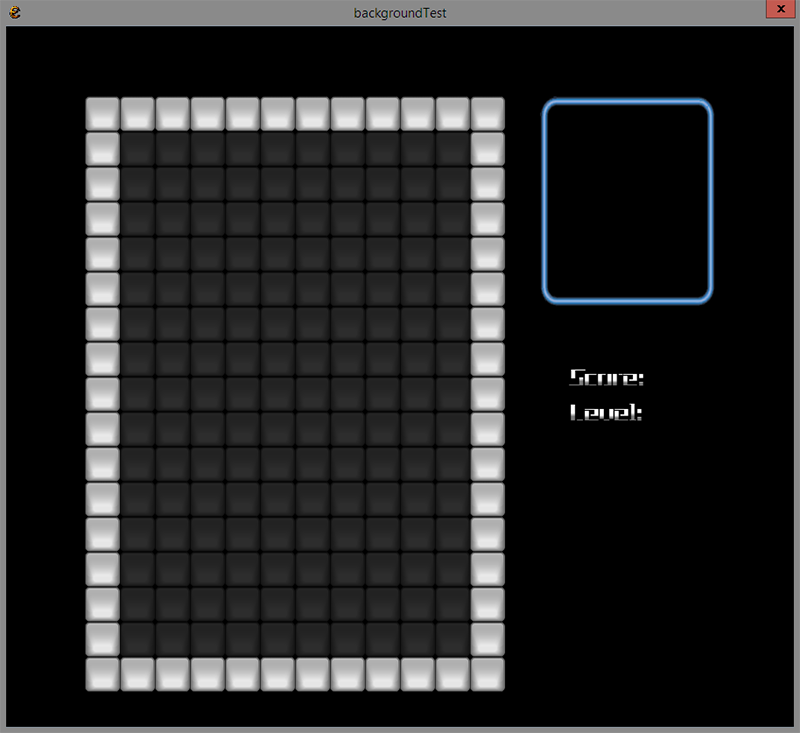
\includegraphics[width=0.6\linewidth]{images/tetris_background.png}
\caption[]{De tetris achtergrond}
\label{fig:tetris_background}
\end{figure}

Om het speelveld te tekenen gebruiken we squares. Dat had ook een afbeelding kunnen zijn, maar zo houden we de interface conform met het spel. Daarnaast heb je een \eeClass{Rect} nodig om een afbeelding te tonen op de plaats waar het volgende blok verschijnt. Tot slot moeten we de positie weten waar we de score en het level tonen.

\begin{code}
class background
{
   Mems<square> squares;
   Rect blockRect;
   Vec2 scorePos;
   Vec2 levelPos;
   
   void create()
   {
   }
   
   void draw()
   {
   }
}

background Background;
\end{code}

In je testprogramma kan je nu al de twee functies van deze class tonen. Daarnaast voeg je de volgende regel toe aan de functie \eeFunc{InitPre}:

\begin{code}
D.mode(WINDOW_WIDTH, WINDOW_HEIGHT);
\end{code}

Deze regel zorgt ervoor dat het window van de applicatie de grootte krijgt die we bij de definitie van de constanten ingaven. Bij de vorige testprogramma's was dat nog niet nodig, maar bij de achtergrond willen we wel zien wat het uiteindelijke resultaat is.

\subsection{Speelveld}

Zoals je weet is het speelveld een grid. Omdat we ook een `muur' rond het speelveld tekenen, beginnen we niet op positie 0 maar op positie -1 met het toevoegen van squares. De squares in het veld zelf geven we het type \eeFunc{BT\_BACKGROUND}. De muren krijgen het type \eeFunc{BT\_WALL}. Daardoor zullen ze in een andere kleur op het scherm gezet worden.

De code om de nodige squares toe te voegen krijg je kado. Eigenlijk is ze niet zo moeilijk, maar wel als je er voor het eerst aan moet beginnen. Lees deze code dus goed en vraag uitleg als je niet begrijpt hoe ze werkt. Daarna voeg je ze toe aan de functie \eeFunc{create}.

\begin{code}
for(int x = -1; x <= SQUARES_PER_ROW; x++)
{
	 for(int y = -1; y <= ROWS; y++)
	 {
			if(x == -1 || y == -1 || x == SQUARES_PER_ROW || y == ROWS)
			{
				 squares.New().create(VecI2(x, y), BT_WALL);
			} else
			{
				 squares.New().create(VecI2(x, y), BT_BACKGROUND);
			}
	 }
}
\end{code}

In de draw functie begin je met het scherm zwart te maken. Daarna toon je alle elementen van de container squares. Test je programma en controleer het resultaat.

\subsection{Next Block}
Op de plaats waar het volgende blok verschijnt plaatsen we een afbeelding. We hebben daar al een constante \eeFunc{WAITPOS} voor gemaakt. Maar dat is een positie in de grid. We moeten die dus steeds vermenigvuldigen met de grootte van een square (de constante \eeFunc{SQUARE\_SIZE}). Daar komt ook nog bij dat we pas mogen tellen vanaf het speelveld, en dat is de constante \eeFunc{GAMEAREA}.

Om te beginnen kunnen we daarom de volgende positie berekenen:

\begin{code}
Vec2 blockPos = GAMEAREA + (WAITPOS * SQUARE_SIZE);
\end{code}

Maar zoals je weet heb je voor een rechthoek een minimum en een maximum nodig. Als minimum trekken we van de gevonden positie twee squares af. Het zou logisch zijn om dan voor de maximum positie twee squares extra te rekenen. Later zal je zien dat dat er visueel minder goed uit ziet, maar dat kan je dan zelf aanpassen. De laatste regel gebruikt de twee nieuwe waarden om de eigenlijke rechthoek in te stellen.

\begin{code}
Vec2 min = blockPos - (2 * SQUARE_SIZE);
Vec2 max = blockPos + (2 * SQUARE_SIZE);
blockRect.set(min, max);
\end{code}

Voeg nu aan de functie \eeFunc{draw} code toe om de afbeelding `tetris\_score' te tekenen via de rechthoek die je net berekende.

\subsection{Tekst}
Je hebt nog twee posities nodig: \eeFunc{scorePos} en \eeFunc{levelPos}. Voor de positie van de score neem je blockPos als uitgangspunt. Van de vertikale waarde trek je vier maal de \eeFunc{SQUARE\_SIZE} af. Voor de level positie vertrek je van de gevonden positie voor de score, maar trekt van de vertikale waarde nog eens \'e\'en square af.

Als je dat in orde hebt kan je te score op het scherm tekenen. Voorlopig zet je daar enkel een tekst. De echte score voegen we later toe. Er is trouwens ook een speciaal font voorzien om in dit spel te gebruiken. Dat is het bestand gui $\Rightarrow$ tetrisFont $\Rightarrow$ tetris Style. Als je niet meer weet hoe je het uitzicht van een tekst moet aanpassen, kan je dat nakijken in hoofstuk \ref{chapter:tekstopmaak}.

Test uiteindelijk weer je programma.

\section{Het geluid}
De volgende class die we maken is \eeClass{soundManager}. Die is behoorlijk eenvoudig en je kan die zelf uitwerken. Er zijn geen create functies nodig, enkel functies die een bepaald geluid afspelen. Je voorziet de volgende functies:

\begin{enumerate}
  \item startMusic: start de soundtrack in een loop.
	\item blip: speelt het `blip' geluid.
	\item score: speelt het `rowdone' geluid.
	\item win: speelt het `won' geluid.
	\item lost: speelt het `lost' geluid.
	\item rotate: speelt het `rotate' geluid.
	\item moveDown: speelt het `down' geluid.
\end{enumerate}

Ook van deze class heb je maar \'e\'en object nodig, dus je maakt onder je class het object \eeClass{SoundManager}. Daarna kan je een eenvoudig testprogramma maken waarin je door op toetsen te drukken deze geluiden afspeelt. Zorg ervoor dat alle geluiden ongeveer even luid klinken. Indien nodig pas je in je class het volume van bepaalde geluiden aan.

\chapter{Application States}
\label{chapter:application_states}

Een application state is een ``status'' van het programma. Wanneer twee delen van een programma nooit gecombineerd worden, dan kan je er twee afzonderlijke application states van maken. 

Wat veel voorkomt is bijvoorbeeld een game lobby en het eigenlijke spel. Je zal nooit de elementen van een game lobby combineren met het spel, dus kan je die volledig scheiden. Ook een login module kan een afzonderlijke application state zijn.

Elk programma heeft al een default application state. Die bestaat uit de functies \texttt{Init()}, \texttt{Shut()}, \texttt{Update()} en \texttt{Draw()}. Wanneer een state actief wordt, dan wordt \texttt{Init()} uitgevoerd. Daarna worden \texttt{Update()} en \texttt{Draw()} afwisselend uitgevoerd, totdat je het programma sluit of overgaat naar een andere state. Op dat moment wordt \texttt{Shut()} uitgevoerd.

\section{Intro}
Voor elke state maak je een afzonderlijk bestand. Bijvoorbeeld voor een intro state:

\begin{code}
bool InitIntro() {return true;}

void ShutIntro() {}

bool UpdateIntro()
{
   if(Time.stateTime()>3 || Kb.bp(KB_ESC)) {
      StateMenu.set(1.0);                    
   }
   return true;
}

void DrawIntro()
{
   D.clear(BLACK);
   D.text (0, 0, "Intro");
}

State StateIntro(UpdateIntro, DrawIntro, InitIntro, ShutIntro);
\end{code}

Je ziet dat dit veel lijkt op de standaard states in je programma. We voegen gewoon het woord Intro toe aan Init, Shut, Update en Draw. Dit houdt het overzichtelijk.

De eigenlijke state zit in de laatste regel:

\begin{code}
State StateIntro(UpdateIntro, DrawIntro, InitIntro, ShutIntro);
\end{code}

Daar geef je aan dat er een nieuwe gamestate is (\eeFunc{StateIntro}) die de typische functies voor een programma bevat. Een \eeFunc{InitPre()} functie kan je niet toelaten, die dient enkel voor de echte start van het programma.

Kijk ook even naar de constructor van \eeFunc{State}:

\begin{code}
State(Bool (*update)(), void (*draw)(), Bool (*init)()=NULL, void (*shut)()=NULL); 
\end{code}

Komt de asterisk (*) je bekend voor? Inderdaad, we hebben met pointers te maken. Pointers naar functies in dit geval. De constructor verwacht dat we aangeven waar de functies voor deze state staan. We verwijzen dus naar de functies die we net gemaakt hebben: \eeFunc{UpdateIntro()} en \eeFunc{DrawIntro()}. Je zegt eigenlijk ``zolang deze state actief is, voer je \eeFunc{UpdateIntro()} uit in plaats van de gewone \eeFunc{Update()} functie.

De volgende twee argumenten, voor de functies \eeFunc{InitIntro()} en \eeFunc{ShutIntro()} zijn optioneel. Je mag ze weglaten als er niets bijzonders moet gebeuren op dat moment.

\begin{note}
Indien een functie argument eindigt met \eeFunc{=NULL}, dan mag je het weglaten.
\end{note} 

\section{Menu}
De code hierboven bevat ook een verwijzing naar StateMenu:

\begin{code}
   if(StateActive.time()>3 || Kb.bp(KB_ESC)) {
      StateMenu.set(1.0);                    
   }
\end{code}

Met andere woorden: we wachten tot de huidige state 3 seconden actief is, of totdat de gebruiker op escape drukt. Dan zetten we een nieuwe application state actief met een crossfade van 1 seconde.

Deze nieuwe state zou er zo kunnen uitzien:
\begin{code}
bool InitMenu() {return true;}
void ShutMenu() {}

bool UpdateMenu()
{
   if(Kb.bp(KB_ESC))return false;
   if(Kb.bp(KB_ENTER))StateGame.set(0.5);
   return true;
}

void DrawMenu()
{
   D.clear(GREY);
   D.text (0,  0  , "Menu");
   D.text (0, -0.3, "Press Enter to start the game");
   D.text (0, -0.5, "Press Escape to exit");
}

State StateMenu(UpdateMenu, DrawMenu, InitMenu, ShutMenu);
\end{code}

Deze state lijkt sterk op de vorige. Maar dit maal kunnen we met Enter naar de game zelf. En dat is dan ook weer een nieuwe application state: \eeFunc{StateGame}.

\section{Game}
Deze code kan je voor \eeFunc{StateGame} gebruiken. Maak ook nu weer een afzonderlijk bestand.
\begin{code}
bool InitGame() {return true;}
void ShutGame() {}

bool UpdateGame()
{
   if(Kb.bp(KB_ESC))StateMenu.set(1.0);
   return true;
}

void DrawGame()
{
   D.clear(TURQ);
   D.text (0, 0, "Game");
}

State StateGame(UpdateGame, DrawGame, InitGame, ShutGame);
\end{code}

Door tijdens de game op escape te drukken, schakelen we terug naar \eeFunc{StateMenu}. In deze state ga je bij een echte game natuurlijk nog heel veel code moeten toevoegen.

\section{Default State}
Dan rest ons nog het starten van het programma. We hebben nu alle nodige states, maar \eeFunc{StateIntro} moet nog actief worden. Dit gebeurt door in de \eeFunc{Init()} functie van het programma dadelijk door te schakelen naar \eeFunc{StateIntro}. De functies \eeFunc{Update()} en \eeFunc{Draw()} worden in dit programma dus niet gebruikt.

\begin{code}
void InitPre()
{
   EE_INIT();
}

bool Init()
{
   StateIntro.set();
   return true;
}

void Shut() {}
bool Update() {return false;} // unused
void Draw  () {             } // unused
\end{code}

\begin{exercise}
Gebruik de code van dit hoofdstuk om een programma te maken dat wisselt tussen de voorziene application states. Elke state plaats je in een afzonderlijk bestand.
\end{exercise}

\chapter{GameLogic}
Er rest ons nog \'e\'en class, maar dan wel de belangrijkste. We hebben alle onderdelen voor het spel klaar, maar die moeten nu samengebracht worden zodat het spel zich gedraagt zoals we verwachten. De class \eeClass{gameLogic} dient precies daar voor. Het framework ziet er zo uit:

\begin{code}
class gameLogic
{
private:
   // blocks in the game
   block currentBlock;
   block nextBlock   ;

   float forceDownCounter = 0         ;
   float slideCounter     = SLIDE_TIME;
   
   // to move a block completely down
   bool  toBottom      = false;
   float toBottomTimer = 0.05 ; 
   
   
   bool canRotate            (C block & b               ) C {}
	 bool canMove              (C block & b, DIRECTION dir) C {}
   void handleBottomCollision()   {}   
   void changeFocusBlock     ()   {}    
   void checkLoss            () C {}
   void handleInput          ()   {}
    
public:
   void create()   {}
   void update()   {}
	 void draw  () C {}
} 
gameLogic GameLogic;
\end{code}

Laten we eerst even de variabelen bekijken:

\begin{description}
	\item[currentBlock] Dit is het blok dat je beweegt tijdens het spel.
	\item[nextBlock] Dit is het volgende blok, dat klaar staat aan de rechterzijde.
	\item[forceDownCounter] Wanneer we het blok niet zelf naar beneden bewegen, dan moet dat na een korte tijd vanzelf gebeuren. Met deze timer regelen we hoe lang dat duurt.
	\item[slideCounter] In tetris kan je wanneer een blok de pile raakt, nog heel even het blok opzij plaatsen. Daar hebben we dus ook een timer voor nodig.
	\item[toBottom] Wanneer we op de spatiebalk drukken moet het blok helemaal naar beneden bewegen. Maar je moet het wel zien bewegen, dus je mag het niet zomaar in \'e\'en keer beneden plaatsen. Met deze bool houden we bij of het huidige blok snel naar beneden moet.
	\item[toBottomTimer] En die beweging heeft ook weer een timer nodig voor elke stap.
\end{description}

\section{De eenvoudige functies}
\subsection{CheckLoss}
Een functie die je zonder problemen kan uitwerken is \eeFunc{checkLoss}. Deze functie moet controleren of de speler het spel verloren heeft. Wanneer gebeurt dat? Wanneer in tetris een nieuw blok bovenaan verschijnt en dat blok kan niet naar beneden verplaatst worden, dan heeft de speler verloren. En wanneer kan een blok niet naar beneden verplaatst worden? Wanneer het zou botsen met de \eeClass{Pile}. 

Pile heeft al een functie \eeFunc{collides}. Aan die functie kan je dus het object \eeClass{currentBlock} doorgeven en de gewenste richting. Geeft de functie false als resultaat, dan kan je de \eeFunc{Score.gameIsLost()} uitvoeren.

\subsection{Create}
De create functie dient om bij de start van een spel alle variabelen een beginwaarde te geven. Je voegt als eerste regel dit toe:

\begin{code}
Random.randomize();
\end{code}

De bedoeling van deze regel is het volgende. Computers hebben een groot probleem met willekeurige getallen. Dat concept past eigenlijk niet binnen een computerlogica. We lossen dat op met het \eeFunc{Random} object, maar dat object heeft eigenlijk intern een lijstje met getallen die het \'e\'en voor \'e\'en af gaat. Elke keer je om een random getal vraagt, krijg je gewoon het volgende getal uit de lijst. Zou je dus je programma elke keer laten beginnen aan het begin van dat lijstje, dan krijg je steeds dezelfde `willekeurige' getallen. Dat maakt je spel na verloop van tijd wel erg voorspelbaar. De functie \eeFunc{randomize} zorgt er voor dat je naar een willekeurige plaats in de lijst springt. Zo krijg je steeds een andere reeks getallen.

\begin{note}
Moest je ooit software ontwikkelen voor een casino, dan zal je nooit de standaard random functies van de programmeertaal mogen gebruiken. Het is namelijk niet zo moeilijk om een programma te schrijven dat, na ingave van de eerste drie resultaten, opzoekt waar de lijst startte. Op dat moment kan je al behoorlijk goed voorspellen wat het volgende getal in de lijst zal zijn. Aangezien een casino toch ook winst wil maken, gebruikt men voor dat soort software een meer complexe random library.
\end{note}

De volgende statements zorgen voor twee willekeurige blokken:

\begin{code}
currentBlock.create(STARTPOS, (BLOCK_TYPE)Random(BT_NUM));
nextBlock   .create(WAITPOS , (BLOCK_TYPE)Random(BT_NUM));
\end{code}

Je ziet dat we de constanten \verb|STARTPOS| en \verb|WAITPOS| gebruiken om de posities in te stellen. Het tweede argument is het blok type. We willen telkens een willekeurig blok, dus we gebruiken de random functie. Het argument van \eeFunc{Random} bepaalt het hoogste getal. Maar die waarde is niet inclusief: dat wil zeggen dat je, als je bijvoorbeeld \eeFunc{Random(3)} schrijft, het resultaat 0, 1 of 2 kan zijn. Niet 3 dus. Waarom schrijven we hier dan \verb|BT_NUM|? Daarvoor moet je even terug in het bestand `enumerations' kijken. \verb|BT_NUM| is het achtste element in de lijst. Het eerste element is gelijk aan 0, dus het achtste element is gelijk aan 7. De \eeFunc{Random} functie zal hier dus een getal van 0 tot en met 6 teruggeven. En omdat een enumeratie niets anders is dan een naam voor een getal, kunnen we dat getal eenvoudig terug omzetten naar een \verb|BLOCK_TYPE|. Want dat is het type dat de create functie verwacht.

Na deze statements moeten we \eeFunc{forceDownCounter} de waarde 0 geven, en slideCounter gelijk stellen aan \verb|SLIDE_TIME|. Die statements kan je zelf wel verzinnen. Tot slot voer je ook de \eeFunc{init} functies van \eeClass{Pile} en \eeClass{Score} uit.

\subsection{Draw}
De draw functie van deze class moet drie elementen op het scherm tonen: het huidige blok, het blok in de wachtpositie en de pile. Voeg de statements toe om dat te doen.

\section{Iets moeilijker}

\subsection{Can Rotate}
We hebben al functies om bij een verplaatsing collisions met de pile of het speelveld te controleren. Nu moeten we ook controleren of het mogelijk is om een blok te roteren. Daarvoor dient de functie \eeFunc{canRotate}.

In deze functie maken we eerst een nieuw blok. We willen namelijk het blok dat we als functie argument binnen krijgen niet roteren, maar enkel controleren of het mogelijk is. Bij dat nieuwe blok voeren we de create functie uit, met als argument het bestaande blok \verb|b|. Daarna roteren we het nieuwe blok.

Nu kunnen we controleren of dit nieuwe blok botst met \eeClass{Wall} of \eeClass{Pile}. Het tweede argument is dan de richting \verb|D_NONE|, want we willen geen verplaatsing controleren. Wanneer een van die functies aangeeft dat er een collision is, dan is het functieresultaat \verb|false|. In het andere geval wordt het \verb|true|.

\subsection{Can Move}
De functie \eeFunc{canMove} zorgt er voor dat we een verplaatsing in \'e\'en keer kunnen controleren. We moeten namelijk zowel collisions met de wall als met de pile in de gaten houden. Als een van deze functies \verb|false| als resultaat heeft, dan is het functieresultaat ook \verb|false|. Is dat niet zo, dan is het resultaat \verb|true|. De argumenten van de functies kan je gewoon doorgeven aan de collide functies van \eeClass{Wall} en \eeClass{Pile}.

\subsection{Change Focus Block}
Op het moment dat een blok beneden is, moet je het toevoegen aan de pile en bovenaan een nieuw blok tonen. Het type van de blok moet gelijk zijn aan het blok in de wachtpositie. Daarna moet je ook nog een beslissen wat nu het volgende blok zal worden.

Je kan deze functie in drie stappen uitwerken:

\begin{enumerate}
	\item Voeg het huidige blok toe aan de pile.
	\item Voer opnieuw de create functie van het huidige blok uit. Als eerste argument gebruik je de constante \verb|STARTPOS|. Het tweede argument is het type van het blok op de wachtpositie. (Zoek in de class \eeClass{block} naar een functie die je dat type geeft.)
	\item Voer nu ook opnieuw de create functie van `nextBlock' uit. Die is gelijk aan het statement dat je eerder in de create functie van deze class schreef.
\end{enumerate}

\subsection{Handle Bottom Collision}
Deze functie beschrijft wat er moet gebeuren als een blok de pile raakt. Ook dat zijn vier eenvoudige statements:

\begin{enumerate}
	\item Voer de functie \eeFunc{changeFocusBlock} uit.
	\item Controleer of er rijen verwijderd kunnen worden uit de Pile.
	\item Geef het aantal verwijderde lijnen (het resultaat van de vorige regel) door aan het \eeClass{Score} object.
	\item Controleer via de functie \eeFunc{checkLoss} of het spel gedaan is.
\end{enumerate}

\subsection{Handle Input}
We hebben ook een functie nodig die reageert wanneer we een toets indrukken. Dat is de functie \eeFunc{handleInput}. Elke toets die we kunnen indrukken tijdens het spel moet hier behandeld worden. Zo moet, wanneer je de pijltjestoets naar beneden indrukt, eerst gecontroleerd worden of een verplaatsing naar beneden wel mogelijk is. Als dat zo is, dan verplaats je het blok naar beneden en laat je een geluidje horen. Dat kan zo:

\begin{code}
if(Kb.bp(KB_DOWN))
{
	 if(canMove(currentBlock, D_DOWN))
	 {
			currentBlock.move(D_DOWN);
			SoundManager.blip();
	 }
}
\end{code}

De code om een blok naar links of rechts te verplaatsen is gelijkaardig. Die werk je dus weer zelf uit.

De `UP' toets gebruik je in tetris om een blok te roteren. Voeg dus ook code toe om te controleren of deze toets wordt ingedrukt. Dit maal moet je enkel de functie \eeFunc{canRotate} uitvoeren met het huidige blok. Als het resultaat van die functie \verb|true| is, dan roteer je het blok en laat je weer een geluidje horen.

En als laatste is er de spatiebalk. Bij het indrukken van de spatiebalk moet een blok helemaal tot beneden bewegen. Om dat te doen geven we de variabele `toBottom' de waarde \verb|true| en de variabele `toBottomTimer' de waarde 0. En ook hier speelt er weer een geluid.

\section{Update}
En dan komen we bij de laatste functie, die het centrum van het spel vormt: de functie \eeFunc{update}. Die functie voert achtereenvolgens verschillende controles uit. 

\subsection{Force Down}
Eerst kijken we of het tijd is om een blok naar beneden te verplaatsen. Daarvoor moeten we de `forceDownCounter' verhogen. Als die hoger is dan de huidige game speed, dan moet het blok een stap naar beneden:

\begin{code}
forceDownCounter += Time.d();
if(forceDownCounter > Score.getSpeed())
{
	 if(canMove(currentBlock, D_DOWN))
	 {
			currentBlock.move(D_DOWN);
			forceDownCounter = 0;
	 }
}
\end{code}

\subsection{Slide Counter}
De slide counter dient om het blok nog even opzij te kunnen bewegen wanneer het de pile raakt. Daarom moeten we eerst weten of het blok de pile raakt en dat is het geval als het niet meer naar beneden kan. In dat geval zullen we de waarde van `slideCounter' verlagen. Als de slideCounter nul wordt, dan voeren we de functie \eeFunc{handleBottomCollision} uit.

\begin{code}
if(!canMove(currentBlock, D_DOWN))
{
	 slideCounter -= Time.d();
} else
{
	 slideCounter = SLIDE_TIME;
}

if(slideCounter <= 0)
{
	 slideCounter = SLIDE_TIME;
	 handleBottomCollision();
}
\end{code}

\subsection{To Bottom}
De bool `toBottom' is \verb|true| wanneer de speler op de spatiebalk drukte. We verplaatsen het blok dan snel naar beneden, maar dat moet nog steeds stap voor stap gebeuren om zichtbaar te zijn. We gebruiken dus een counter met een kleine waarde waar we telkens weer de tijdsdelta van aftrekken. Elke keer dat de counter nul wordt verplaatsen we het blok een positie naar beneden. Als dat niet meer mogelijk is, dan schiet de bovenstaande code (Slide Counter) in actie.

Enkel wanneer het blok niet naar beneden glijdt, controleren we de input van de speler.

\begin{code}
if(toBottom)
{
	 toBottomTimer -= Time.d();
	 if(toBottomTimer < 0)
	 {
			toBottomTimer = 0.05;
			if(canMove(currentBlock, D_DOWN))
			{
				 currentBlock.move(D_DOWN);

			} else
			{
				 toBottom = false;
			}
	 }
} else
{
	 handleInput();
}
\end{code}

Daarmee is ook deze functie af. Het enige wat je nu nog moet doen is de \eeFunc{create}, \eeFunc{update} en \eeFunc{draw} toevoegen aan de Game State. En daarna natuurlijk alle fouten oplossen tot je programma werkt zoals het hoort.

\section{Nabespreking}
Je hebt nu een volledig project uitgewerkt. Hopelijk zal je onthouden hoe belangrijk het is om alles in classes onder te brengen. Ook het gebruik van testprogramma's is erg belangrijk om een groot project goed uit te werken.

Maar natuurlijk komt deze manier van werken niet helemaal overeen met de realiteit. De auteur van deze cursus wist precies wat er moest gebeuren en in welke volgorde je dat het best kon aanpakken, nog voor je aan deze oefening begon. Als je zelf aan een project begint dan is dat wel anders. Het is heel gewoon dat je de classes die je vooraf maakt meermaals moet aanpassen. Dikwijls blijken er toch nog functies te ontbreken, of schrijf je functies die je uiteindelijk niet nodig blijkt te hebben. Dat is, zeker voor een beginnende programmeur, heel normaal.

Enkel door ervaring leer je steeds beter inschatten welke functies een class nodig zal hebben. En zelfs dan kan je dat niet altijd exact voorspellen.

\part{Gui}
\chapter{Gui}

Een grafische user interface (Gui) kan je visueel ontwerpen via de gui editor. Maar om je interface te gebruiken in je applicatie zal je wel moeten programmeren.
Bekijk eerst hoe je de gui editor gebruikt. Je kan daarvoor gebruik maken van deze youtube tutorial:

\url{https://www.youtube.com/watch?v=eFsBxC6pGxE}

\section{Een gui laden}

Voor elk window maak je best een afzonderlijk code bestand, dat houdt het overzichtelijk. In dat bestand begin je een class, die bij voorkeur dezelfde naam heeft als de Gui en het bestand. 

\begin{code}
// Een class voor een login window
class loginWindow
{
private:
	 // een GuiObjs object kan een Gui object bevatten
	 // dat je maakt via de editor.
   GuiObjs objs;
   
public:
   // Deze create functie zullen we later in het programma
	 // uitvoeren om het login window te laden.
   void create()
   {
	    // het GuiObjs object kan je gebruiken om een gui te
			// laden. Met de functie load kan je hier via drag and 
			// drop een GUI object plaatsen.
      objs.load( --- Drop Gui Object here --- );
      
			// Uiteindelijk voeg je deze gui toe aan de Gui Manager
      Gui += objs;
   }
   
}

// aangezien je normaal gezien maar 1 object nodig hebt van elke gui class,
// kan je dat hier al maken.
loginWindow LoginWindow;
\end{code}

De bovenstaande code laad je gui in het geheugen en voegt die toe aan de Gui manager. In je programma ga je dan de \texttt{create()} functie uitvoeren en de Gui updaten en tekenen.

\begin{code}
void InitPre()
{
   EE_INIT();
}

bool Init()
{
   // voor elk gui object voer je de create functie uit
   // tijdens de Init fase
   LoginWindow.create();
   return true;
}

void Shut() {}

bool Update()
{
   // Wanneer je een of meerdere gui classes gebruikt, dan 
   // update je de Gui manager tijdens de applicatie update
   Gui.update();
   return true;
}

void Draw()
{
   D.clear(WHITE);
   
   // Wanneer je een of meerdere gui classes gebruikt,  dan
   // laat je de Gui manager alles op het scherm tekenen. Je
   // doet dit op het einde van de Draw functie,  omdat de 
   // de Gui boven op de andere objecten hoort.
   Gui.draw();
}
\end{code} 

\begin{exercise}
Maak een login window (met naam, wachtwoord textlines en een ok en cancel button) en zorg via bovenstaande code dat het in een programma op je scherm verschijnt.
\end{exercise}

\section{Pointers naar elementen}
Je hebt nu wel een gui geladen, maar je wil waarschijnlijk ook de elementen van de gui gebruiken. Maar die zitten in \texttt{GuiObjs objs}. Je maakt daarom pointers aan naar elk element waar je iets mee wil doen. Na het laden van de gui zoek je naar de elementen en wijs je die toe aan de gewenste pointer.

\begin{code}
class loginWindow
{
private:
   GuiObjs objs;
	 // een pointer naar een Window, met de naam window
	 Window * window;
	 // een pointer naar een Button, met de naam buttonClose
	 Button * buttonClose;
   
public:

   void create()
   {
      objs.load( --- Drop Gui Object here --- );
			// zoek in objs naar een Window met de naam "window"
      window = objs.findWindow("window");
			// zoek in objs naar een Button met de naam "buttonClose"
			buttonClose = objs.findButton("buttonClose");
			
      Gui += objs;
   }
   
}
loginWindow LoginWindow;
\end{code}

Je mag je elementen noemen zoals je wil, maar de naam waar je naar zoekt (met findWindow, findButton, \ldots) moet wel gelijk zijn aan de naam die je het element in de Gui Designer hebt gegeven. Als je toch een verkeerde naam zoekt, dan zal je pointer nergens naar verwijzen. Als je dan later die pointer gebruikt in het programma, dan zal je applicatie crashen.

Eens een pointer verwijst naar een element, kan je hem gebruiken in je code. Het volgende voorbeeld gebruikt de pointer naar het window om dit te tonen en te verbergen:

\begin{code}
class loginWindow
{
private:
   GuiObjs objs;
	 Window * window;
	 Button * buttonClose;
   
public:

   void create()
   {
      objs.load( --- Drop Gui Object here --- );
      window = objs.findWindow("window");
			buttonClose = objs.findButton("buttonClose");
			
			// verberg het window na het laden
			window.hide();
			
      Gui += objs;
   }
	
	 // deze functie kan je eender waar in je programma gebruiken
	 void show() {
			// dit zorgt voor een fade in van je window	
	    window.fadeIn();
   }
}
loginWindow LoginWindow;
\end{code}

De bovenstaande code laat je toe om bijvoorbeeld in de update functie van je applicatie de volgende code te plaatsen:

\begin{code}
if(Kb.bp(KB_F5)) LoginWindow.show();
\end{code}

\section{Callback functies}
Sommige gui elementen, zoals buttons, kan je een functie toewijzen. Die functie wordt dan automatisch uitgevoerd bij een actie. Bij een button is die actie het moment dat iemand klikt op de button. Bij een slider is het het moment waarop de slider verplaatst wordt. Een TextLine heeft dan weer een actie als iemand de waarde aanpast.

De functie die je toewijst aan een element kan eender welke naam hebben, maar het formaat moet wel juist zijn. Je moet de functie declareren als \texttt{static void} en met als argument een referentie naar de class die je maakt. Bijzonder aan een \texttt{static} functie is dat die geen rechtstreekse toegang heeft tot de objecten in je class. Daarom is de referentie naar de class noodzakelijk. Wanneer je de functie doorgeeft aan de button, gebruik je \eeClass{T} om het object door te geven waar de functie bij hoort. Andere functies of elementen van de class moet je dus ook via die referentie benaderen.

\begin{code}
class loginWindow
{
private:
   GuiObjs objs;
	 Window * window;
	 Button * buttonClose;
    
	 // Deze functie wordt uitgevoerd wanneer iemand
	 // op de button klikt.
   static void myButtonFunction(loginWindow & obj) {
		  obj.window.fadeOut();
	 }
	
public:

   void create()
   {
      objs.load( --- Drop Gui Object here --- );
      window = objs.findWindow("window");
			buttonClose = objs.findButton("buttonClose");
			window.hide();
			
			// Wijs de functie hierboven toe aan de button
			buttonClose.func(myButtonFunction, T);
      Gui += objs;
   }
	
	 void show() {
	    window.fadeIn();
   }
}
loginWindow LoginWindow;
\end{code}

\begin{note}
Pas op. De editor maakt een fout als je de naam van een functie typt: er komen vanzelf haakjes achter. Wanneer je een functie gebruikt hoort dat zo, maar in dit geval moet je enkel de naam doorgeven. Verwijder de haakjes dus.
\begin{code}
buttonClose.func(myButtonFunction(), T); // fout!
buttonClose.func(myButtonFunction, T);   // juist.
\end{code}
\end{note}
(
\begin{exercise}
Vul de vorige oefening aan met de mogelijkheid om je login window te tonen en te verbergen via de functietoets F1. Zorg ook dat zowel de ok als de cancelbutton het window terug sluiten.
\end{exercise}

\section{De inhoud van een element}
\label{chapter:gui_content}
Dikwijls heeft een element ook een inhoud. Een \texttt{TextLine} heeft een tekst als inhoud. Een \texttt{Slider} heeft een waarde tussen 0 en 1, afhankelijk van zijn positie. Een \texttt{CheckBox} heeft als inhoud \texttt{true} wanneer aangevinkt, of \texttt{false} indien niet. 

Die inhoud opvragen kan complex zijn. Stel je voor dat we een \texttt{TextLine} hebben:

\begin{code}
TextLine tl;
\end{code}

De waarde vragen vraag je dan op met:

\begin{code}
Str waarde = tl();
\end{code}

Eenvoudig! Maar\ldots\ meestal hebben we geen \texttt{TextLine} in onze code, maar een \textbf{pointer} naar zo'n element. Dus moet je aangeven dat je wil werken met het element waar die pointer naar verwijst. Dat kan zo:

\begin{code}
Str waarde = (*tl)();
\end{code}

Als je dan ook nog eens vanuit een \texttt{static void} functie werkt, zoals een functie die wordt uitgevoerd wanneer je op een knop klikt, dan moet je ook het object van de class meegeven. Bij de class \texttt{loginWindow} van hierboven wordt dat dan:

\begin{code}
Str waarde = (*LoginWindow.tl)();
\end{code}

Je kan de inhoud van een element ook wijzigen. Dat is gelukkig een stuk eenvoudiger:

\begin{code}
Str waarde = "mijn tekst";
tl.set(waarde);
// of in een static void functie
LoginWindow.tl.set(waarde);
\end{code}

Een verder uitgewerkt voorbeeld van het loginWindow zou er zo kunnen uitzien:

\begin{code}
class loginWindow
{
private:
   GuiObjs objs;
	 Window * window;
	 Button * buttonLogin;
   TextLine * tlName;
	 TextLine * tlPass;
	
   static void tryLogin(loginWindow & obj) {
	    Str name = (*obj.tlName)();
			Str pass = (*obj.tlPass)();
			
			if(Equal(name, "john") && Equal(pass, "secret")) {
			   obj.window.fadeOut();
		  }
	 }
	
public:

   void create()
   {
      objs.load( --- Drop Gui Object here --- );
      window = objs.findWindow("window");
			buttonLogin = objs.findButton("login");
			tlName = objs.findTextLine("name");
			tlPass = objs.findTextLine("pass");
			
			window.hide();
			buttonClose.func(tryLogin, T);
			
      Gui += objs;
   }
	
	 void show() {
	    window.fadeIn();
   }
}
loginWindow LoginWindow;
\end{code}

\begin{exercise}
Maak een programma met een login window. De achtergrond van het programma is zwart, maar wordt wit wanneer je ingelogd bent. Je toont dan ook de login naam op het scherm via \texttt{D.text()}. Als uitbreiding kan je ook eens naar een andere application state overschakelen na het inloggen.
\end{exercise}

\section{Data en interface: Never mix!}
Een belangrijke regel bij het schrijven van een GUI is de volgende:

\begin{note}
GUI en data houd je strikt gescheiden.
\end{note}

Een GUI dient om data aan te passen. Maar die data zelf hoort \textbf{NOOIT} (nooit) thuis in de gui class. Je maakt dus steeds een afzonderlijke class voor de data. Je gebruikt dan functies in je gui class om die data te lezen en te wijzigen. Een voorbeeld:

\begin{code}
// een data class voor een player
class player {
private:
   Str name;
	 int age;

public:
   void setName(C Str & name) { T.name = name; }
	 void setAge (int     age ) { T.age  = age ; }
	 Str  getName(            ) { return   name; }
	 int  getAge (            ) { return   age ; }
	
	 void draw() {
	    D.text(0,    0, S + "name: " + name);
			D.text(0, -0.1, S + "age : " + age );
	 }
}
player Player;
\end{code}

\begin{code}
// een GUI class
class changePlayerGUI {
private:
   GuiObjs objs;
	 Window   * window  ;
	 TextLine * tlName  ;
	 TextLine * tlAge   ;
	 Button   * buttonOK;
	
public:
   void create() {
	    objs.load( -- drop gui object here ---);
			window   = objs.findWindow  ("window");
			tlName   = objs.findTextLine("name"  );
			tlAge    = objs.findTextLine("age"   );
			buttonOK = objs.findButton  ("ok"    );
			
			buttonOK.func(changeData, T);
			tlName  .set(        Player.getName() );
			tlAge   .set(TextInt(Player.getAge ())); // converteer int naar Str met TextInt()
			
			Gui += objs;
   }
	
	 static void changeData(changePlayerGUI & obj) {
	    Str name = (*obj.tlName)();
	 	  Str age  = (*obj.tlAge )();
	 	  int ageInt = TextInt(age);
	 	  Player.setName(name  );
	 	  Player.setAge (ageInt);
   }
}

changePlayerGUI ChangePlayerGUI;
\end{code}

\chapter{Gui Window}
Alhoewel je gui elementen ook direct op het scherm kan zetten, plaats je ze meestal in een window. Zelfs al wil je dat window niet tonen (je kan het later onzichtbaar maken) is dit de meest eenvoudige manier om elementen bij mekaar te houden. Wil je bijvoorbeeld verschillende elementen samen tonen of verbergen, dan plaats je ze best samen in een window.

\section{Definitie}
Kijk eens naar de definitie van een \eeClass{Window}:

\begin{code}
const_mem_addr struct Window : GuiObj // Gui Window !! must be stored in constant memory address !!
{
   Byte      flag       ,
   ...
\end{code}

De commentaar en ook het eerste woord \eeFunc{const\_mem\_addr} laten je weten dat een window een vast geheugen adres nodig heeft. Wat betekent dat? Wel, je mag een window nooit opslaan in een gewone container. De elementen van een \eeClass{Memc} kunnen wel eens naar een andere locatie in het geheugen verplaatst worden zonder dat je dat zelf merkt. Voor GUI elementen mag zoiets niet gebeuren.

Nu is dat meestal geen probleem. Wanneer je een GUI ontwerpt dan wil je van elk window en de elementen daarin meestal maar \'e\'en object maken en dat doe je dan onder de declaratie van de class die je daarvoor maakt. (In het vorige hoofdstuk was dat \verb|loginWindow LoginWindow|). Op die manier heb je automatisch een vast geheugen adres. Heb je toch een container met meerdere objecten van deze class nodig? Gebruik dan de container \eeClass{Memx} of \eeClass{Meml}.

Wat ook opvalt is het laatste woord: \eeClass{GuiObj}. Dat betekent dat een Window gebaseerd is op de class \eeClass{GuiObj}. Alle eigenschappen van deze class zijn dus ook beschikbaar in \eeClass{Window}. We zeggen daarom dat \eeClass{GuiObj} de base class van \eeClass{Window} is.

\section{Class Methods}
Als je verder in de definitie van de class \eeClass{Window} kijkt, dan zie je heel wat lidfuncties. En daar komen ook de lidfuncties van \eeClass{GuiObj} nog bij. Zolang je je gui ontwerpt met de gui editor, zal je de meeste van deze functies niet zo vaak nodig hebben. We bespreken hier enkele functies die toch handig kunnen zijn:

\begin{description}
	\item[\eeFunc{setTitle(C Str \&title)}] Via deze functie kan je de titel van het window wijzigen.
	\item[\eeFunc{fadeIn()}] Samen met de functie \eeFunc{fadeOut()} bepaal je de zichtbaarheid van een window.
	\item[\eeFunc{showing()}] Samen met de functie \eeFunc{hiding()} controleer je de zichtbaarheid van een window. Je kan bijvoorbeeld de pijltjestoetsen enkel gebruiken om je avatar te bewegen wanneer een window niet zichtbaar is.
	\item[\eeFunc{button[3]}] is geen functie. Een window bevat altijd die buttons met een specifiek doel: minimize, maximize en close. De typische buttons die je vaak in de rechterbovenhoek ziet. Als je deze buttons wil tonen, dan kan je na het laden van je window de \eeFunc{show()} functie van de gewenste buttons uitvoeren.
\end{description}

\begin{exercise}
Maak in programma waarin je een window toont zolang de spatiebalk ingedrukt is. Wanneer het window zichtbaar is, dan stel je de titel van het window gelijk aan de tijd dat je programma loopt. (Gebruik de functie \eeFunc{Time.appTime()}.)
\end{exercise}

Er is nog een functie die bijzondere aandacht verdient: de functie \eeFunc{pos(C Vec2 \&pos)} van de base class \eeClass{GuiObj}. Deze functie komt vaak van pas om de positie van je window te corrigeren. Je kan in de gui editor wel de positie van een window bepalen, maar dat is vaak niet voldoende. Je wil bijvoorbeeld een window aan de linkerkant van het scherm, maar niet ieder scherm heeft dezelfde aspect ratio. Daarom bereken je best de positie voordat je een window toont. Voor de linkerbovenhoek zou dat er zo uit zien:

\begin{code}
void show() {
   window.pos(Vec2(-D.w(), D.h());
	 window.fadeIn();
}
\end{code}

Andere posities vragen dikwijls iets meer werk. Dan moet je immers ook de afmetingen van het window in rekening brengen. Gelukkig kan dat eenvoudig via de lidfunctie \eeFunc{rect()}. Die geeft je informatie over de grootte van je window, dat natuurlijk een rechthoek is. In dit voorbeeld zie je hoe je een window aan de linkeronderhoek van het scherm plaatst. 

\begin{code}
void show() {
   Vec2 pos;
	 pos.x = -D.w();
	 pos.y = -D.h() + window.rect().h();
   window.pos(pos);
	 window.fadeIn();
}
\end{code}

\begin{exercise}
Plaats een window aan de rechterkant van het scherm, in het midden. Maak ook een tweede functie \eeFunc{showCentered()} die het window in het midden van het scherm toont.
\end{exercise}

\section{Dialogs}
Esenthel bevat ook enkele windows met en meer specifiek doel. Een daarvan is de class \eeClass{Dialog}. Als je naar de declaratie van die class kijkt, dan zie je dat een \eeClass{Dialog} de class \eeClass{Window} als basis heeft. Dat betekent dat ook de functies van \eeClass{GuiObj} beschikbaar zijn.

Een dialog zal je niet een de gui editor ontwerpen. De lidfunctie \eeFunc{autoSize()} wordt gebruikt om na het instellen van de tekst en de buttons alle elementen voldoende plaats te geven. Dat betekent dat je in dit geval geen \eeClass{GuiObjs} en ook geen pointers gebruikt. Hier een voorbeeld:

\begin{code}
class confirmExit {
private:
   Dialog dialog;
   
   static void cancelFunc(confirmExit & obj)
   {
      obj.dialog.fadeOut();
   }
   
   static void proceedFunc(confirmExit & obj)
   {
      Exit();
   }
      
public:
   void create() {
      Mems<Str> buttonTexts;
      buttonTexts.New() = "cancel";
      buttonTexts.New() = "proceed";
      dialog.create("Exit?", "Ben je zeker dat je dit programma wil sluiten?", buttonTexts);
      dialog.autoSize();
      dialog.hide();
      
      dialog.buttons[0].func(cancelFunc, T);
      dialog.buttons[1].func(proceedFunc, T);
      
      Gui += dialog;
   }
   
   void show() {
      dialog.fadeIn();
   }
}

confirmExit ConfirmExit;
\end{code}

\begin{exercise}
Voeg deze class toe aan een programma en toon de dialog wanneer de gebruikt op escape drukt, in plaats van daar dadelijk het programma af te sluiten.
\end{exercise}


\chapter{Gui Buttons}

De meest gebruikte functie van de class button is \eeFunc{func()}. Daarmee koppel je een callback functie aan de button. Die functie wordt dan uitgevoerd wanneer je op de button klikt. In de inleiding werd dit al besproken, maar denk er aan dat dit een statische functie moet zijn, die dus los staat van het eigenlijke object. Alhoewel het niet strikt noodzakelijk is, geef je dus best altijd een referentie naar het huidige object door aan de button. 

Enkele andere handige functies zijn:

\begin{description}
	\item[\eeFunc{enabled(bool enabled)}] laat je toe om op bepaalde momenten een button non-actief te maken.
	\item[\eeFunc{setText(C Str \&text)}] wijzigt de tekst van een button.
	\item[\eeFunc{bool sound}] door deze eigenschap op `true' te zetten, wordt er een geluid afgespeeld wanneer je op deze button drukt. Het geluid zelf kan je instellen via \eeClass{Gui.click\_sound\_id}. Standaard is dat geluid leeg, maar je kan er eender welk geluidsbestand aan toewijzen. (Let op, dit is geen functie maar een property!)
\end{description}

\begin{exercise}
Pas de vorige oefening aan, zodat de buttons in je dialog een geluid afspelen.
\end{exercise}

\section{Toggle Buttons}
Een button kan ook gebruikt worden als toggle button. In dat geval gedraagt die zich net iets anders. Een enkele toggle button kan je als alternatief voor een checkbox gebruiken. Bijvoorbeeld om bepaalde elementen op het scherm te tonen. Hieronder zie je een voorbeeld van een toggle button die een crosshair aan of uit zet.

\begin{code}
class crossHair
{
private:
   Button button;
   bool on = false;
   
   static void buttonFunc(crossHair & obj)
   {
      obj.on = obj.button();
   }
   
public:
   void create()
   {
      button.create(Rect(-D.w() + 0.1, D.h() - 0.2, -D.w() + 0.6, D.h() - 0.1), "cross on/off");
      button.mode = BUTTON_TOGGLE;
      button.set(false);
      button.func(buttonFunc, T);
      Gui += button;
   }
   
   void draw()
   {
      if(!on) return;
      Circle(0.1).draw(RED, false);
      Edge2(0, -0.12, 0, 0.12).draw(RED);
      Edge2(-0.12, 0, 0.12, 0).draw(RED);
   }
}

crossHair CrossHair;
\end{code}

Enkele zaken vallen wellicht op in deze class. Ten eerste wordt de gui editor niet gebruikt. Om slechts \'e\'en button op het scherm te tonen zou dat wat omslachtig zin. Daarom is de Button geen pointer, maar een echt object. We dienen dan wel zelf de functie \eeFunc{create} uit te voeren, met als argument een rechthoek en een tekst.

Daarna wordt de mode aangepast, zodat we een toggle button krijgen. En via de set functie zetten we de huidige stand op `uit'. De statische functie \eeFunc{buttonFunc} geeft de stand van de button door aan de bool `on'. Via haakjes na de naam van de button kom je dus zijn huidige stand te weten. Dit is enkel zinvol bij toggle buttons. Een gewone button heeft immers geen stand.

\begin{exercise}
Voeg deze code toe aan een programma. Kies zelf een geschikte positie voor de button. Wanneer je tijdens de create functie de button zou inschakelen met \eeFunc{button.set(true)} dan zal de crosshair niet toch niet getoond worden. Zoek uit hoe dat komt en hoe je dat kan oplossen.
\end{exercise}
\chapter{CheckBox}
Een checkbox verschilt niet zoveel van een button in toggle modus. Welk van de twee je gebruikt, maakt enkel visueel een verschil. Net zoals alle gui classes is ook \eeClass{CheckBox} afgeleid van \eeClass{GuiObj}, dus je kan ook alle functies van die base class gebruiken.

\begin{exercise}
Maak een window met enkele checkboxes. De eerste checkbox verbind je aan een functie die een bool `showFPS' controleert. Wanneer die \eeFunc{true} is, dan toon je via de huidige fps op het scherm met behulp van de functie \eeFunc{Time.fps()}. Gebruik de andere checkboxes om enkele windows uit de vorige oefeningen te tonen en verbergen.
\end{exercise}


\chapter{Slider}

Een slider heeft een waarde tussen 0 en 1, afhankelijk van zijn positie. Je kan die waarde opvragen via de operator \eeFunc{()}. Voor een gewone slider wordt dat:

\begin{code}
float value = mySlider();
\end{code}

Maar wanneer je slider een pointer is, dan moet je wel aangeven dat je niet de pointer maar het object zelf wil aanspreken:

\begin{code}
float value = (*mySlider)();
\end{code}

Doe je dat dan vanuit een static functie die je koppelt aan de slider, dan wordt die variabele automatisch aangepast wanneer je de slider beweegt. Zo kan je het volgende schrijven:

\begin{code}
class sliderWindow
{
private:
   GuiObjs objs;
	 Window * window;
	 Slider * speedSlider;   
	 float currentSpeed = 1;	
	
   static void speedSliderFunction(sliderWindow & obj) {
		  currentSpeed = (*obj.speedSlider)() * 5;
	 }
	
public:
   void create()
   {
      objs.load( --- Drop Gui Object here --- );
      window = objs.findWindow("window");
			speedSlider = objs.findSlider("speedSlider");

			speedSlider.func(speedSliderFunction, T);
      Gui += objs;
   }
}
sliderWindow SliderWindow;
\end{code}

\begin{note}
Sliders geven altijd een waarde tussen 0 en 1. Je kan die schaal niet aanpassen, maar je kan wel het resultaat vermenigvuldigen tot de range die je nodig hebt. Wil je bijvoorbeeld een waarde tussen 10 en 50, dan schrijf je:

\begin{code}
float value = 10 + slider() * 40;
\end{code}
\end{note} 

\begin{exercise}
Maak een window met drie sliders en een \eeClass{Color}. De color stel je in het begin gelijk aan BLACK, maar de sliders wijzigen respectievelijk de r, g en b waarden van de color. Teken dan ook de achtergrond in deze kleur.
\end{exercise}
\chapter{TextLine}
TextLine is de enige gui class die je kan gebruiken om tekstinvoer van de gebruiker te krijgen. De visuele functies (grootte, positie, zichtbaarheid enzovoort) zijn identiek aan de andere classes die je zag. Maar de functie \eeFunc{func} werkt anders. Je kan daar op dezelfde manier een functie aan koppelen, maar waar bij een button of een checkbox de functie getriggerd wordt door een mouse click, zal een tekstline deze functie uitvoeren bij elke muisklik. Dat valt eenvoudig te demonstreren met de volgende code:

\begin{code}
Str myText;

// Om dit voorbeeld kort te houden wordt de gui class verder niet uitgewerkt.
// Je ziet enkel de callback functie.

void MyTextLineFunc(guiClass & obj) {
  myText = (*obj.myTextLine)();
}

// .. en de Draw functie
void Draw() {
	D.clear(BLACK);
	D.text(0, 0, myText);
}
\end{code}

Als je de invoer enkel wil controleren op een bepaald moment, dan kan je een button gebruiken en pas dan de invoer van de TextLine controleren. Een voorbeeld daarvan vind je in hoofdstuk \ref{chapter:gui_content}.

\section{Tekst omzetten naar een getal}

De inhoud van een TextLine is steeds een tekst, ook al bestaat die tekst uit cijfers. Als je die inhoud als een integer of float wil gebruiken, dan moet je die eerst converteren. Daarvoor bestaan er functies als \eeFunc{TextInt} en \eeFunc{textFlt}. 

\begin{code}
int   i = TextInt( (*obj.myTextLine)() );
float f = TextFlt( (*obj.myTextLine)() );
\end{code}

Let wel op: als je textline niet omgezet kan worden naar een getal, dan krijg je geen foutmelding. Het resultaat is dan steeds 0.

\section{Andere handige functies}
Wanneer je een tekst in een TextLine wil plaatsen, dan kan dat met de functie \eeFunc{set}. Die aanvaardt een string als argument:

\begin{code}
Str purpose = "life";
int meaning = 42;

myTextLine .set(purpose);
myTextLine2.set(S +  42);
\end{code}

Met de functie \eeFunc{password} kan je sterretjes in plaats van letters tonen:

\begin{code}
myTextLine.password(true);
\end{code}

Via de functie \eeFunc{clear} maak je een textline leeg:

\begin{code}
myTextLine.clear();
\end{code}

\begin{exercise}
TextLine heeft ook een functie \eeFunc{cursor} om de positie van de cursor op te vragen en aan te passen. Maak een programma met een tekstline waarin je een tekst plaatst. Maak ook functies \eeFunc{moveLeft} en \eeFunc{moveRight} die de cursor een positie naar links of naar rechts kunnen verplaatsen. In de \eeFunc{Update} functie van je class zorg je dat de cursor via F1 en F2 naar links en rechts verplaatst kan worden. Via F3 zet je de password modus aan of uit, en via F4 maak je het hele veld leeg.

Tot slot zoek je in de header file op hoe je tekst selecteert. Zorg er voor dat je via F5 de hele tekst selecteert, en via F6 de selectie ongedaan maakt.
\end{exercise}












\part{Data}
\chapter{Data opslaan in een bestand}
Je kan data op verschillende manieren bewaren. Tekstbestanden zijn eenvoudig om te lezen, maar minder efficient om data in op te slaan. Je kan data ook binair opslaan, wat minder plaats in beslag neemt. Maar die bestanden kan je dan weer niet eenvoudig controleren met een tekst editor.

\section{Locaties}
Wat je ook kiest, je zal eerst moeten bepalen waar je data opslaat. Het is geen goed idee om zelf het hele path naar je bestand vast te leggen in code. Stel je voor dat je beslist om een config bestand op te slaan op \verb|C:\myGame\gameData\config.txt.| Dat is nogal vervelend als de gebruiker je app verplaatst naar een andere directory of schijf. De gebruiker verwacht dat de data op zijn minst in een subdirectory van je game zit. Het is zelfs mogelijk dat een computer geen C drive heeft!

Esenthel laat je toe om bepaalde paden op te vragen. Zo kan je de `documents' folder van de betreffende computer en gebruiker opvragen, zonder dat je zelf het hele path moet kennen:

\begin{code}
Str docPath = SystemPath(SP_DOCUMENTS);
\end{code}

Als je daarna een bestand wil opslaan in die `documents' folder, dan kan je het path daarvoor als volgt samenstellen:

\begin{code}
Str documentPath = S + docPath + "/myfile.txt";
\end{code} 

\begin{note}
Merk op dat je een forward slash (/) gebruikt om folders te schrijven. In Windows gebruik je normaal een backslash, maar Esenthel zal die zelf omzetten. De bedoeling is dat je met deze engine een app kan maken die ook op andere systemen --zoals Linux, mac of Android-- werkt. Andere systemen gebruiken steeds een forward slash.
\end{note}

Naast \verb|SP_DOCUMENTS| kan je nog andere systeempaden opvragen:

\begin{itemize}
\item \textbf{SP\_DESKTOP} verwijst meestal naar \verb|C:/Users/*/Desktop|.
\item \textbf{SP\_APP\_DATA} verwijst naar \verb|C:/Users/*/AppData/Roaming|. Op mobiles is het het path waar een applicatie toelating heeft om data te bewaren.
\item \textbf{SP\_APP\_DATA\_EXTERNAL} verwijst ook  naar \verb|C:/Users/*/AppData/Roaming|. Maar indien een mobile system een externe SD kaart heeft, dan zal dat path gebruikt worden.
\item \textbf{SP\_ALL\_APP\_DATA} verwijst meestal naar \verb|C:/ProgramData|
\end{itemize}

Een volledig overzicht van de mogelijkheden vind je in de header file \verb|Misc $\Rightarrow$ Misc| onder de enum declaratie `SYSTEM\_PATH'. Niet alle paden zijn beschikbaar op elk systeem. Je kan bijvoorbeeld niet naar de desktop schrijven op een mobiel platform.

\begin{exercise}
Controleer waar de bovenstaande paden op jouw computer naar verwijzen. Maak een eenvoudig testprogramma dat de resulterende string voor elk van deze paden op het scherm toont. \textsl{(Project Textfiles, ex. 01)}
\end{exercise}

\section{TextData}

De class \eeClass{TextData} laat je toe op een eenvoudige manier data als text op te slaan. Deze class is vooral voor het bewaren van config files erg handig.

\subsection{Content bewaren}
Data opslaan is eenvoudig. Voor elke variabele die je wil bewaren maak je een `node'. Je kent aan die node een waarde toe, en vervolgens sla je het bestand op.

\begin{code}
TextData data;
data.getNode("name").setValue("John Doe");
data.getNode("highscore").setValue("100");
data.save(S + SystemPath(SP_DOCUMENTS) + "/config.txt");
\end{code} 

De functie \eeFunc{getNode} zal zoeken naar de naam van de node. Indien er nog geen node bestaat met die naam, dan wordt er een nieuwe node gemaakt. De functie \eeFunc{setValue} geeft de nieuwe node een waarde.

Het bestand zal de volgende inhoud bevatten:
\begin{verbatim}
name=`John Doe`
highscore=100
\end{verbatim}

\begin{exercise}
Maak een programma met de variabelen \texttt{name}, \texttt{address}, en \texttt{age}. Geef de variabelen een default waarde en sla ze op in een bestand. Controleer of het bestand de juiste waarden bevat.
\end{exercise}

\subsection{Een bestand laden}
Een bestand laden doe je zo:

\begin{code}
TextData data;
Str docPath = SystemPath(SP_DOCUMENTS);
data.load(S + docPath + "\config.txt");
\end{code}

Indien het bestand bestaat, zal het via de bovenstaande code ingelezen worden. \textsl{(De functie \eeFunc{load} geeft ook een bool als resultaat die aangeeft of dit gelukt is. In een echte applicatie controleer je best die waarde.)}

\subsection{Content lezen}
Om de inhoud van een bestand te lezen, moet je het eerst laden. Daarna kan je je zoeken naar een bepaalde node, en de inhoud van die node toewijzen aan een variabele. Omdat het altijd mogelijk is dat een node niet bestaat, neem je twee voorzorgsmaatregelen:

\begin{enumerate}
	\item Geef je variabele een default waarde. Wanneer het niet lukt om de node te laden, blijft deze waarde gewoon behouden.
	\item Haal enkel de waarde uit een node wanneer de node bestaat. Data uit een onbestaande node halen crashed je programma.
\end{enumerate}

\begin{code}
// config values
Str name = "new player";
int highScore = 0;
int credits = 100;

TextData data;
Str docPath = SystemPath(SP_DOCUMENTS);
if(data.load(S + docPath + "/config.txt")) {
   TextNode * node;
	 
	 // try finding the name
	 node = data.findNode("name");
	 if(node) {
	    name = node.asText();
	 }
	 
	 // try finding the highscore
	 node = data.findNode("highscore");
	 if(node) {
	    highScore = node.asInt();
	 }
}
\end{code}

\begin{note}
Wanneer je een node bewaart, dan kan je er eender welk type aan toekennen met de functie \eeFunc{setValue}. Maar bij het laden van een node moet je wel een onderscheid maken naargelang het type: je gebruikt \eeFunc{asInt} voor een integer, en \eeFunc{asText} voor een string. Meer mogelijkheden vind je in de header file File $\Rightarrow$ Xml. (\eeClass{TextNode} is gebaseerd op \eeClass{TextParam}.)
\end{note}

\begin{exercise}
Pas het bestand uit de vorige oefening aan via een texteditor en laadt het terug in je programma. Toon de waarden van de variabelen op het scherm. Controleer of ze correct zijn.  \textsl{(Project Textfiles, ex. 02)}
\end{exercise}

\subsection{Een class voor een config file}
Tot slot krijg je hier nog een volledig uitgewerkt voorbeeld waarop je kan voortbouwen als je je eigen config file wil maken. De bedoeling is dat je de \verb|load()| functie uitvoert bij het starten van je programma en de \verb|save()| functie bij het afsluiten. Daartussen kan je de variabelen wijzigen via de voorziene functies. \textsl{(Project Textfiles, ex. 03)}

\begin{code}
class configFile {
private:
  Str name      = "new player";
	int highscore = 0  ;
	int credits   = 100;
	
public:
  Str getName     () { return name     ; }
	int getHighscore() { return highscore; }
	int getCredits  () { return credits  ; }
	
	void setName     (C Str & name   ) { T.name      = name   ; }
	void setHighscore(  int   score  ) { T.highscore = score  ; }
	void setCredits  (  int   credits) { T.credits   = credits; }
	
	void load() {
	  TextData data;
		if(data.load(S + SystemPath(SP_APP_DATA) + "/mygame/config.txt")) {
		  TextNode * node;
			
			if(node = data.findNode("name"     )) name      = node.asText();
			if(node = data.findNode("highscore")) highscore = node.asInt ();
			if(node = data.findNode("credits"  )) credits   = node.asInt ();
	  }
  }
	
	void save() {
	  TextData data;
		data.getNode("name"     ).setValue(name     );
		data.getNode("highscore").setValue(highscore);
		data.getNode("credits"  ).setValue(credits  );
		
		data.save(S + SystemPath(SP_APP_DATA) + "/mygame/config.txt");
  }
}
configFile ConfigFile;
\end{code}	

\section{Binary Files}
De TextData files hierboven zijn vooral handig voor configuratiebestanden of andere bestanden die je ook wil kunnen openen in een tekst editor. Ze zijn niet de meest effici\"ente manier om data op te slaan. Met de class \verb|File| kan het veel compacter. Met \verb|File| sla je enkel de waarde van een variabele op, zonder een ID om die terug te vinden:

\begin{code}
File f;                  // create file object
f.write("file.dat"    ); // start writing to a file
f.putInt(128          ); // write an integer
f.putFlt(3.14         ); // write a float
f.putStr("Hello world"); // schrijf een tekst naar het bestand
\end{code}

Wanneer je nadien de data terug wil inlezen, dan doe je dat in dezelfde volgorde. De functie \eeFunc{readTry} zorgt er voor dat de waarden enkel gelezen worden wanneer het bestand bestaat. Er bestaat ook de functie \eeFunc{read}, maar die crashed het programma wanneer een ongeldig bestand wordt gelezen.

\begin{code}
File f;
if (f.readTry("file.dat")) {
	int   i    = f.getInt();
	float pi   = f.getFlt();
	Str   text = f.getStr();
}
\end{code}

\begin{exercise}
Maak een gui class met een \eeClass{TextLine}, een \eeClass{Slider}, een \eeClass{CheckBox} en twee \eeClass{Button}'s. De eerste button bewaart de huidige waarde van de gui elementen in een bestand. De tweede button laadt dat bestand opnieuw en kent de opgeslagen waarden toe aan de gui elementen. Wijzig de gui na het opslaan en controleer of na het laden alle elementen terug de juiste waarde hebben. 
\end{exercise}

\subsection{Data Order}
Wat als je data in een andere volgorde leest en schrijft? Bekijk even de volgende code:

\begin{code}
void save() {
  File f;
	f.write("trouble.dat");
	f.putBool(true);
	f.putInt (12  );
}

void load() {
  File f;
	f.read("trouble.dat");
	int i = f.getInt ();
	int b = f.getBool();
}
\end{code}

Bij het laden en opslaan van de data werd een andere volgorde gebruikt. De compiler zal deze fout niet opmerken. Een bool variabele is precies 1 bit groot, maar een integer bestaat uit 32 bits. Er worden dus 33 bits opgeslagen: 1 + 32. Bij het laden wordt eerst de integer gelezen, maar vooraan in het bestand staat de bool variabele. Het programma laadt dus 32 bits, maar dat zijn de bool en 31 bits van de integer. Daarna wordt de laatste bit van de integer gelezen als bool. Figuur \ref{fig:filebits} illustreert dit.

\begin{figure}[ht]
\centering
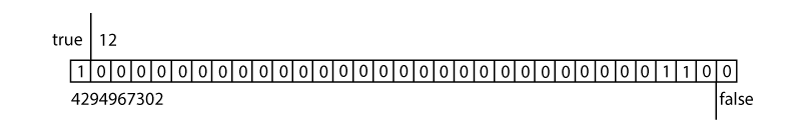
\includegraphics[width=0.8\linewidth]{../images/filebits}
\caption[]{bits in een bestand}
\label{fig:filebits}
\end{figure}

\begin{note}
De volgorde van de variabelen bij het lezen en het schrijven van een \verb|File| moet exact dezelfde zijn. Als je daar fouten tegen maakt, dan kan je programma crashen of zich anders gedragen dan je zou verwachten. 
\end{note}

En er is nog een andere, minder opvallende manier waarop dit mis kan gaan. C++ behandelt de argumenten van een functie van rechts naar links (net zoals de meeste andere programmeertalen, overigens). Als voorbeeld een stukje code.

\begin{code}
float r = 0.1;
float x = 0.3;
float y = 0.4;

Circle c;
c.set(r, x, y);
\end{code}

Argumenten worden gelezen van rechts naar links. Dat betekent dat de instructie \eeFunc{pos2.set} op de volgende manier wordt uitgevoerd:

\begin{enumerate}
	\item Geef de waarde van y aan het derde argument van set.
	\item Geef de waarde van x aan het tweede argument van set.
	\item Geef de waarde van r aan het eerste argument van set.
	\item Voer de functie set uit.
\end{enumerate}

Waarom is deze volgorde belangrijk? Wel, in het bovenstaande voorbeeld helemaal niet. De data die we gebruiken is niet sequentieel, ze moet niet in de juiste volgorde gelezen worden. We kunnen op elk moment de waarden van x, y of r raadplegen. Maar wat als we data uit een bestand halen? 

\begin{code}
float r = 0.1;
float x = 0.3;
float y = 0.4;

// Put data in an imaginary file
f.putFlt(r);
f.putFlt(x);
f.putFlt(y);

// ... after loading this data
Circle c;
c.set(f.getFlt(), f.getFlt(), f.getFlt());
\end{code}

De eerste float in het bestand bevat de waarde voor r. De tweede de waarde voor x en de derde voor y. Dit voorbeeld lijkt op het eerste zicht te werken, maar omdat functieargumenten van rechts naar links verwerkt worden, komt de eerste float rechts terecht. Op de plaats waar we y verwachten! Je lost dit op door er voor te zorgen dat de inhoud stap voor stap gelezen wordt. In dit geval kan dat door vooral de functie set niet te gebruiken.

\begin{code}
Circle c;
c.r     = f.getFlt();
c.pos.x = f.getFlt();
c.pos.y = f.getFlt();
\end{code}

\begin{exercise}
Maak een kort programma dat deze fout demonstreert. (Je gebruikt dus opzettelijk de foute manier.) \textsl{(Project Textfiles, ex. 04)}
\end{exercise}

\subsection{Objecten Opslaan}
Je kan ook meerdere objecten opslaan in hetzelfde bestand. Om dit te doen, geef je een \eeClass{File} object door als referentie. Zo bijvoorbeeld in de volgende class:

\begin{code}
class resource {
  int type  ;
	Vec pos   ;
	int amount;
	
	void create(int type, int amount, C Vec & pos) {
	  T.type   = type  ;
		T.pos    = pos   ;
		T.amount = amount;
	}
	
	// ... other functions are omitted to keep this example short ...
	
	void save(File & f) {
	  f.putInt(type  );
		f.putFlt(pos.x ).putFlt(pos.y).putFlt(pos.z);
		f.putInt(amount);
	}
	
	void load(File & f) {
	  type   = f.getInt();
		pos.x  = f.getFlt();
		pos.y  = f.getFlt();
		pos.z  = f.getFlt();
		amount = f.getInt();
	}
}	
\end{code}

Vervolgens voorzie je een manager class om die resources te beheren. Naast functies om ze toe te voegen, te verwijderen, op het scherm te tekenen etc., voeg je functies toe om alle bestaande resources op te slaan of te laden:

\begin{code}
class resourceManager {
  Memx<resource> resources;
	
	void save() {
		File f;
		f.write("resources.dat");
		
		f.putInt(resources.elms());
		FREPA(resources) {
			resources[i].save(f);
		}
	}
	
	void load() {
	  File f;
		if(f.readTry("resources.dat")) {
			
			int elms = f.getInt();
			for(int i = 0; i < elms; i++) {
				resources.New().load(f);
			}
		}
	}
}

resourceManager RM;
\end{code}

Je kan zelfs alle data voor je programma opslaan in hetzelfde bestand, door ook in de manager class de File als referentie door te geven in plaats van ze ter plaatse te defini\"eren. In dat geval zou je bijvoorbeeld op de volgende manier je data opslaan:

\begin{code}
void save() {
  File f;
	f.write("allData.data");
	Config.save(f);
	RM    .save(f);
}

void load() {
	File f;
	f.load("allData.data");
	Config.load(f);
	RM    .load(f);
}
\end{code}

\begin{exercise}
Maak een class voor een cirkel die ook zijn kleur kan onthouden. Voorzie een manager class die cirkels kan bevatten. Elke klik met de muis voegt een cirkel toe aan de manager, op de huidige positie van de muis en in een willekeurige kleur. (Herlees hoofdstuk \ref{section:managerClass} indien nodig.)

Zorg dat bij het afsluiten van het programma alle cirkels bewaard worden. Bij de start van het programma laadt je alle cirkels van de vorige sessie. \textsl{(Project Textfiles, ex. 05)}
\end{exercise}



\chapter{Databases}

\section{Database Servers}
Data kan je niet enkel in gewone bestanden opslaan, je kan ook een database gebruiken. De meest voorkomende standaard voor het werken met databases is SQL (sequel). Esenthel Engine ondersteunt 3 verschillende databases: Microsoft SQL, MySQL en SQLite. Elk van deze databases heeft voor- en nadelen.

\begin{itemize}
\item \textbf{Microsoft SQL:} De database server is zeer performant, maar je hebt wel een Windows OS nodig. Tijdens de ontwikkeling zal dit waarschijnlijk geen probleem zijn, maar wanneer je een server voor je programma laat hosten dan is een Windows host duurder.
\item \textbf{MySQL:} Dit is waarschijnlijk de meest gebruikte SQL server. MySQL draait op zowat elk OS, is gratis en open source. De installatie en het onderhoud zijn niet erg moeilijk, en de performantie is OK.
\item \textbf{SQLite:} SQLite gebruikt een gewoon bestand als database. Er moet dus geen server ge\"installeerd worden. Vooral tijdens de ontwikkelfase kan dat een voordeel zijn, maar het zorgt er wel voor dat SQLite heel wat trager is dan een `echte' database server. SQLite kan ook een goede oplossing zijn als je aan de client side data wil opslaan in een database, zonder dat je daarvoor de gebruiker verplicht om een database server te installeren.
\end{itemize}

Een belangrijk voordeel van de database class in Esenthel is dat je makkelijk van database kan wisselen. Je kan dus tijdens het ontwikkelen voor SQLite kiezen en pas achteraf overschakelen op een MySQL of MS SQL database.

\section{Een Database Gebruiken}
\subsection{De Verbinding}
Alvorens je een database kan gebruiken, moet je een verbinding maken. De \texttt{SQL} class laat je toe een verbinding te maken met elk soort database. In het geval van een SQLite database is de naam van een bestand voldoende, maar bij een echte server zal je de host, de naam van de database, een gebruiker en een wachtwoord moeten voorzien. MS SQL en MySQL laten je ook nog toe een pointer naar een string mee te geven. Indien de verbinding niet lukt, zal die string de foutmelding van de database server bevatten.

\begin{code}
SQL sql;
Str messages;

// voor Microsoft SQL
if (!sql.connectMSSQL("LocalHost\\SQLExpress", "test_db", "", "", &messages)) {
  // verbinding mislukt
	Exit(S + "Database error: " + messages);
}

// voor MySQL
if (!sql.connectMySQL("localhost", "test_db", "user", "password", &messages)) {
  // verbinding mislukt
	Exit(S + "Database error: " + messages);
}

// voor SQLite
if (!sql.connectSQLite("test.db")) {
  Exit(S + "Database error");
}
\end{code}

\begin{exercise}
Maak een class \eeClass{database} met een functie \eeFunc{create}. In deze functie maak je een verbinding met een SQLite database met de naam `mydata.db'. Je voegt een je programma een object van de class toe en je voert de functie create uit. Na het uitvoeren van je programma ga je op zoek naar het bestand `mydata.db'. Op het bestand met een SQLite browser, te downloaden via \url{http://sqlitebrowser.org} . (Je zal een foutmelding krijgen omdat de database leeg is.)
\end{exercise}

\subsection{Een tabel maken}
Je programma kan bestaande tabellen gebruiken, of je kan met een andere tool je de tabellen in je database aanmaken. Een derde optie is dat je de database aanmaakt op het moment dat je je programma start. Ook dit kan weer handig zijn tijdens de ontwikkelfase: je controleert of een tabel al bestaat, en indien niet dan laat je je programma die tabel maken. Eventueel kan je er ook via je code wat data in zetten. Op die manier kan je je programma eenvoudig testen. En als je de structuur van je data wil wijzigen, dan verwijder je gewoon de hele database zodat die opnieuw aangemaakt wil worden.

Zoals je weet bestaat een tabel uit kolommen met een naam en een type. Bovendien moet in elke tabel \'e\'en kolom de primary key zijn, eventueel met auto-increment. Je kan ook voor elke kolom een default waarde instellen, maar dat is niet verplicht.

\begin{code}
if(!sql.existsTable("accounts")) {
  // maak een tabel voor accounts
	
	Memc<SQLColumn> columns;
	columns.New().set("ID"      , SDT_INT    ).mode = SQLColumn.PRIMARY_AUTO;
	columns.New().set("name"    , SDT_STR, 32); // een string met maximaal 32 tekens
	columns.New().set("password", SDT_STR, 32);
	columns.New().set("active"  , SDT_BOOL   );
	columns.New().set("score"   , SDT_INT    ).default_val="0";
	
	if(!sql.createTable("accounts", columns, &messages)) {
	  Exit(S + "Can't create table for accounts: \n" + messages);
	}
	
	// voeg test data toe
	SQLValues values;
	values.New("name"    , "freddy"    );
	values.New("password", "kamerplant");
	values.New("active"  , true        );
	
	if(!sql.newRow("accounts", values, &messages)) {
	  Exit(S + "Can't add data to table accounts: \n" + messages);
	}
}
\end{code}

\begin{exercise}
Breidt de functie \eeFunc{create} uit de vorige oefening uit met de bovenstaande code. Voer het programma opnieuw uit en bekijk de database achteraf opnieuw via de SQLite browser. Voeg daarna een extra kolom `lives' toe. Controleer of deze kolom na het uitvoeren ook in de tabel staat.
\end{exercise}

\subsection{Data Lezen}
Als je eenvoudig alle data uit een tabel wil lezen, dan kan dat met de functie \texttt{getAllRows()}. Je wil die data dan waarschijnlijk wel ergens in het geheugen houden, dus daar gebruik je best een class en een memory container voor. Met de table ``accounts'' als voorbeeld zou je een class \texttt{account} kunnen maken om een rij uit de database in het geheugen te zetten.

\begin{code}
class account {
  // Om het voorbeeld kort te houden zijn alle variabelen public.
	// In een echt programma kan je meestal beter set en get functies gebruiken.
	int  ID    ; 
	Str  name  ;
	bool active;
	int  score ;
}
\end{code}

gDe functie \texttt{getAllRows()} gebruik je eenvoudigweg met de naam van een tabel. Na het uitvoeren van de functie bevat het \texttt{sql} object alle rijen van de gevraagde tabel. Met de functie \texttt{getNextRow()} kan je dan een rij met gegevens opvragen totdat er geen volgende rij meer is. Vervolgens kan je de functie \texttt{getCol()} gebruiken om de waarde van een kolom te verkrijgen. 

\begin{note}
Vraag de kolommen van een rij steeds op in de volgorde waarin ze in de tabel staan. Je kan wel kolommen overslaan, maar niet terug gaan naar een vorige kolom.
\end{note}

\begin{code}
Memc<account> accounts;
sql.getAllRows("accounts");

for( ;sql.getNextRow(); ) {
  account & a = accounts.New();
	
	sql.getCol(0, a.ID    );
	sql.getCol(1, a.name  );
	// skip loading the password in column 2
	sql.getCol(3, a.active);
	sql.getCol(4, a.score );
}
\end{code}

\begin{exercise}
	\begin{enumerate}
		\item Maak een class \eeClass{account}.
		\item Maak een class \eeClass{accountManager} waarin je een container voor alle accounts voorziet. 
		\item Voorzie een functie \eeFunc{create} die alle records uit de database leest en toevoegt aan de container. 
		\item Voeg aan de class een integer `currentAccount' toe die je op nul zet. 
		\item Via de functies \eeFunc{next} en \eeFunc{previous} kan je het huidige account wijzigen. Zorg er wel voor dat dit niet kleiner dan nul kan worden, en ook niet groter dan het aantal accounts.
		\item Voorzie een functie draw die de inhoud van het huidige account op het scherm toont.
	\end{enumerate}
\end{exercise}

Je wil niet steeds alle data uit een tabel in het geheugen laden. Dikwijls ben je maar ge\"interesseerd in een of in enkele records. In dat geval gebruik je de functie \texttt{getRows()}. Als argument kan je bij deze functie een voorwaarde opgeven, net zoals je dat in een SQL statement zou doen:

\begin{code}
sql.getRows("accounts", "name='freddy'");
if(sql.getNextRow()) {
	// load column data
}
\end{code}

Dikwijls zal je dergelijke code in een functie gebruiken, en een bepaalde waarde als resultaat geven. Stel je voor dat we van een account de score willen weten. De functie zou er dan zo kunnen uitzien:

\begin{code}
int getScore(C Str & name) {
  int result = 0;
	sql.getRows("accounts", S+ "name='" + name + "'");
	if(sql.getNextRow()) {
	  sql.getCol(4, result);
	}
	return result;
}
\end{code}

\begin{note}
Bij het opstellen van een voorwaarde moet elke waarde tussen enkele quotes staan. Als je dan ook nog variabelen toevoegt aan de vergelijking, dan moet je goed uitkijken dat de quotes op de juiste plaats staan.
\end{note}

Maar je zou ook een hele account als referentie kunnen doorgeven. Dat is vooral bruikbaar in het geval je een volledige record wil laden. We zouden dan eerst de class \texttt{account} uitbreiden:

\begin{code}
class account {
	int  ID      ;
	Str  name    ;
	Str  password;
	bool active  ;
	int  score   ;
	
	bool load(C Str & name) {
		T.name = name;
	  return loadAccount(T);
	}
}
\end{code}

Via de functie load kunnen we een account uit de database halen door een naam mee te geven. De return waarde laat ons ook weten of dat gelukt is. De functie \eeFunc{loadAccount()} kunnen we dan zo uitwerken:

\begin{code}
bool loadAccount(account & a) {
  sql.getRows("accounts", S+"name='"+a.name+"'");
	if(sql.getNextRow()) {
		sql.getCol(0, a.ID);
		sql.getCol(2, a.password);
		sql.getCol(3, a.active);
		sql.getCol(4, a.score);
		return true;
  }
	return false;
}
\end{code}

\begin{exercise}
	\begin{enumerate}
		\item Voeg aan de class \eeClass{database} een de functie \eeFunc{loadAccount} toe.
		\item Maak een Gui class met een TextLine waarin we een naam kunnen schrijven. Voeg ook een Button en Text objects toe om de ID, wachtwoord en score te tonen.
		\item Voorzie een functie die, wanneer de gebruiker op de button klikt, zoekt naar een account met de naam in TextLine en dat account toont in de gui.
	\end{enumerate}
\end{exercise}

\subsection{Records tellen}
Het gebeurt dat je niet in de inhoud van een record ge\"interesseerd bent, maar enkel wil weten of een record bestaat. Wil je eenvoudigweg weten hoeveel records een tabel bevat, dan gebruik je de functie \texttt{getAllRowsNum()}.

\begin{code} {
int accountsInDB() {
  return sql.getAllRowsNum("accounts");
}
\end{code}

\begin{exercise}
Voeg aan de class \eeClass{database} een functie toe die telt hoeveel accounts er zijn. Toon dit ergens op je scherm.
\end{exercise}

Vaker wil je het aantal accounts dat aan een voorwaarde voldoet. Bijvoorbeeld het aantal actieve accounts. Dan gebruik je de functie \texttt{getRowsNum}, die weer een conditie als argument heeft, net zoals \texttt{getRows()}.

\begin{code}
int activeAccountsInDB() {
  return sql.getRowsNum("accounts", "active='true'");
}
\end{code}

Met zo'n voorwaarde kan je ook te weten komen of een combinatie van gegevens bestaat. Zo kan je bijvoorbeeld controleren of een wachtwoord juist is.

\begin{code}
bool validate(C Str & name, C Str & password) {
  int count = sql.getRowsNum("accounts", S + "name='" + name + "' AND password='" + password + "'");
	return (count > 0);
}
\end{code}

\begin{exercise}
Maak een login gui waarin de gebruiker een naam en een wachtwoord kan ingeven. Zorg (met de bovenstaande code als voorbeeld) dat je kan kontroleren of de combinatie correct is en toon dat op het scherm.
\end{exercise}

\subsection{Data Opslaan}
Je zal vrijwel nooit alle gegevens in een database willen overschrijven. Wel wil je regelmatig een record die je aangepast hebt, terug opslaan. Dat kan zo:

\begin{code}
void save(account & a) {
  SQLValues values;
	values.New("name", a.name);
	values.New("password", a.password);
	values.New("active", a.active);
	values.New("score", a.score);
	
	Str messages;
	if(!sql.setRow("accounts", S + "ID='" + a.ID + "'", values, &messages)) {
	  Exit(S + "Error saving account: \n" + messages);
	}
}
\end{code}



Je hoeft ook niet steeds alle data op te slaan. Enkel de waarden die je in \texttt{SQLValues} opneemt, worden aangepast. Zo kan je bijvoorbeeld enkel het wachtwoord opslaan.

\begin{code}
void savePassword(account & a) {
  SQLValues values;
	values.New("password", a.password);
	sql.setRow("accounts", S + "ID='" + a.ID + "'", values);
}
\end{code}

\begin{note}
Pas nooit de primary key van een record aan!
\end{note}

\begin{exercise}
Voeg een Gui toe waarmee de gebruiker zijn wachtwoord kan aanpassen.
\end{exercise}

\subsection{Data Verwijderen}
Tot slot zal je ook records willen verwijderen die je niet meer nodig hebt. Daar kan je de functie \texttt{delRow} voor gebruiken. 

\begin{code}
void removeAccount(int ID) {
  sql.delRow("accounts", S + "ID='" + ID + "'");
}
\end{code}


\chapter{Over netwerk applicaties}
Tegenwoordig heeft bijna elke applicatie wel ergens een netwerk nodig. Bij online games is dat evident, maar ook andere toepassingen houden steeds meer info bij in \textit{'the cloud'}. \textit{(Die cloud is niets meer dan een fancy woord om aan te duiden dat je informatie op een server opslaat.)} Ook wordt een online component dikwijls gebruikt om een licentie te controleren.

Toch is een netwerk applicatie een pak moeilijker te ontwikkelen dan een gewone, stand-alone applicatie. Enkele redenen daarvoor:

\begin{itemize}
\tick Je schrijf niet \'e\'en, maar twee programma's. Er moet namelijk ook een server geschreven worden.
\tick Data die je verstuurt over het netwerk bestaat enkel uit bits. Zowel de client als de server moeten die op dezelfde manier interpreteren.
\tick Een netwerk kan traag en onbetrouwbaar zijn. Je software moet dat zo goed mogelijk opvangen.
\tick Mobile apps hebben dikwijls weinig bandbreedte. Je mag niet meer data versturen dan strikt noodzakelijk is.
\end{itemize}

Het is dan ook erg belangrijk dat je het overzicht bewaart bij het onwikkelen van een netwerk applicatie. In de volgende hoofdstukken zullen we de delen van zo'n programma bestuderen. Hierin staan verschillende technieken beschreven die je helpen dat overzicht te bewaren. In ieder geval is het belangrijk om je project goed te structureren. In figuur \ref{fig:filetree} zie je een file tree van het voorbeeldproject.

\begin{figure}[ht]
\centering
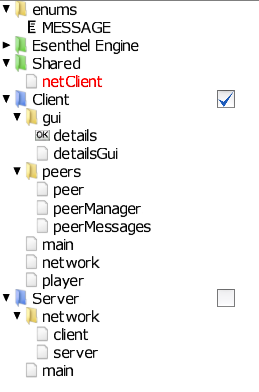
\includegraphics[width=0.3\linewidth]{../images/filetree.png}
\caption[]{Structuur van een client-server project.}
\label{fig:filetree}
\end{figure}

Je ziet dat zelfs een eenvoudig project al snel uit heel wat files bestaat. Je zet die niet allemaal in dezelfde map. Evident is dat we twee applicaties hebben: client en server. Maar het is zeker niet overbodig om ook binnen die applicaties folders te maken voor code die samen hoort. Zo heeft de client een folder voor alle gui elementen \textit{(zowel layout als code)} en een folder voor code i.v.m. peers \textit{(dat zijn andere spelers op het netwerk)}. We plaatsen dus ook de editor componenten niet zomaar in de root van het project. Immers, de server heeft dat gui element `details' helemaal niet nodig. Bij een verdere uitwerking zal de server waarschijnlijk zijn eigen gui elementen nodig hebben, waar de client dan weer niets aan heeft.

Daarnaast zie je ook een folder `enums'. Deze folder is w\'el beschikbaar voor elke app. We gebruiken enumeraties om berichten door te geven tussen de client en de server. Door ze in de root van het project te plaatsen zijn we zeker dat beide applicaties dezelfde lijst gebruiken.

Ook is er een library (groene folder) met de naam `Shared'. In deze folder plaatsen we alle code die zowel bij de client als de server hoort.

\begin{exercise}
Maak een nieuw project aan. Daarin maak je alvast alle folders en bestanden zoals in de afbeelding hierboven.
\end{exercise}

\section{Messages}
Data verzenden over het netwerk doe je via \texttt{Files}. Denk hierbij niet aan grote bestanden zoals op een harde schijf: elk bericht dat je verstuurt over het netwerk is in feite in klein bestandje. 

Aangezien je bij een file dient te vermelden hoe je het wil noemen, voordat je er data in kan zetten, moet je bij een netwerkfile aangeven dat het enkel om het bestand in het geheugen gaat. En omdat de ontvanger van het bericht moet weten over wat voor bericht het gaat, stuur als eerste byte steeds een enum met het type bericht. Hieronder zie je een voorbeeld van een dergelijk bestand, ditmaal om de positie van een speler te verzenden.

\begin{code}
File f;
f.writeMem();
f.putByte(M_CLIENT_POS);
f.putFlt(pos.x);
f.putFlt(pos.y);
\end{code}

Alle netwerkfuncties in de client en de server zullen dus steeds naar de eerste byte van een bericht kijken om te bepalen welke functie het bericht verder zal afhandelen. Je maakt best een enumeratie die alle mogelijke berichten bevat. In een groot programma kan ook een tweede byte geschakeld worden om een verdere onderverdeling te maken.

\begin{exercise} 
Maak in je project een enum `MESSAGE' met de volgende waarden: 
\begin{itemize}
	\item M\_CLIENT\_FULL
	\item M\_CLIENT\_POS
	\item M\_HELLO
	\item M\_ADD\_CLIENT
	\item M\_REMOVE\_CLIENT
\end{itemize}
\end{exercise}



\section{Gedeelde classes}
Je app zal data structuren nodig hebben die zowel bij de client als bij de server bekend zijn. Dat kan bijvoorbeeld een class voor de player zijn, met minstens een naam en een positie. Het zou ook een item in de game wereld kunnen zijn, een chat bericht of een quest. 

Aan de andere kant zijn er ook steeds verschillen tussen de client en de server. Zo zal een player bij de client op het scherm moeten verschijnen, en zal de gebruiker hem kunnen verplaatsen via de muis of het toetsenbord. Bij de server is dat niet wenselijk, maar moet een player wel in een database opgeslagen kunnen worden.

We maken voor dit soort classes een zogenaamde `base class' in de library `Shared'. Het voorbeeld bevat een dergelijke class voor een speler, die we \texttt{netClient} noemen:

\begin{code}
class netClient
{
   int id;
   Str name = "Player";
   Color color = RED;
   Vec2 pos;

   void writePosToFile(File & f)
   {
      f.putFlt(pos.x);
      f.putFlt(pos.y);
   }
   
   void readPosFromFile(File & f)
   {
      pos.x = f.getFlt();
      pos.y = f.getFlt();
   }
      
   void writeDetailsToFile(File & f)
   {
      f.putStr(name);
      f.putByte(color.r).putByte(color.g).putByte(color.b);
      writePosToFile(f);
   }
   
   void readDetailsFromFile(File & f)
   {
      name = f.getStr();
      color.r = f.getByte(); color.g = f.getByte(); color.b = f.getByte();
      readPosFromFile(f);
   }
}
\end{code}

Naast data zoals id, naam, kleur en positie bevat de class ook functies. Als we een bericht over het netwerk versturen, zullen we steeds deze functies gebruiken om de gewenste data aan een \texttt{File} toe te voegen. Zo zijn we zeker dat de client en de server dezelfde data verwachten. Mocht je in een later stadium bijvoorbeeld de snelheid van een speler willen onthouden en die ook meesturen in een `Details' bericht, dan moet je dat enkel hier aanpassen. 

\begin{note}
Het is soms verleidelijk om deze data rechtstreeks in de client of server applicatie naar een bestand te schrijven. Vroeg of laat zal je je echter vergissen, door bijvoorbeeld de volgorde van de data door mekaar te halen. Dat soort fouten is erg moeilijk te debuggen. Maak er daarom een gewoonte van om een gedeelde base class te maken. 
\end{note}

\chapter{De Server}
De server applicatie is verantwoordelijk voor het volgende:

\begin{itemize}
\tick connecties van nieuwe clients aanvaarden;
\tick berichten van bestaande clients aanvaarden en indien nodig doorsturen naar andere clients;
\tick opmerken wanneer een clients offline gaat en dat indien nodig laten weten aan andere clients;
\end{itemize}

Daarnaast is het meestal zo dat data ook opgeslagen wordt in een database, dat er game-events gegenereerd worden, het gedrag van AI's wordt berekend, etc.

\section{Main Program Loop}
Het hoofdprogramma van de server is meestal behoorlijk eenvoudig: je start een server object, update dat regelmatig en tekent eventueel wat op het scherm. Dat laatste is zelfs dikwijls ongewenst, want een serverprogramma draait dikwijls op een server OS zonder gui. We overlopen even de voorbeeld code.

\begin{code}
void InitPre()
{
   EE_INIT();
   App.flag = APP_WORK_IN_BACKGROUND|APP_NO_PAUSE_ON_WINDOW_MOVE_SIZE;
}
\end{code}

De \texttt{InitPre()} functie is niet bijzonder. De Applicatie krijgt enkele flags mee zodat de update functie ook door gaat als het programma geen focus heeft of geminimaliseerd is.

\begin{code}
bool Init()
{
   if(!Server.create())
   {
      Exit("Can't create Server");
   }
   return true;
}
\end{code}

In \texttt{Init()} cre\"eren we het \texttt{Server} object. Die server class moeten we wel zelf schrijven, wat hieronder aan bod komt. Als het niet lukt om de server te starten, dan wordt het programma afgesloten.

\begin{code}
void Shut()
{
   Server.del();
}
\end{code}

Tot nu toe hebben we de \texttt{Shut()} functie vrijwel nooit nodig gehad. Bij een server applicatie moeten we zeker zijn dat de netwerk resources terug vrijgegeven worden als het programma klaar is. Daarom is deze code noodzakelijk.

\begin{code}
bool Update()
{
   if(Kb.bp(KB_ESC))return false;
   Server.update();
	 Time.wait(1);
   return true;
}
\end{code}

De \texttt{Update()} functie update de server. Later zullen waarschijnlijk ook andere updates toegevoegd worden, zoals bijvoorbeeld een AI manager update. Op het eind van de update functie laten we het programma een milliseconde wachten. Zo belasten we de CPU niet harder dan nodig.

\begin{code}
void Draw()
{
   D.clear(TURQ);
   D.text(0, 0.7, S + "Server");
   D.text(0, 0.5, S + "Connected clients: " + Server.clients.elms());
   D.text(0, 0.3, S + "Local Addres: " + Server.addressLocal().asText());
}
\end{code}

Tot slot is er de \texttt{Draw()} functie die ons wat informatie geeft over de server. Het aantal actieve clients en het IP adres van de server.

\begin{note}
In dit voorbeeld gebruiken we het lokale IP adres van de server. Daarmee kan je een client op hetzelfde netwerk verbinden met de server, maar externe verbindingen zijn zo niet mogelijk. Wanneer het tijd is om de toepassing te testen over het internet, dan moet je het globale IP adres gebruiken. Het is mogelijk dat je daarvoor ook de router correct moet configureren.
\end{note}

\section{De server Class}
De server zelf moet je niet zelf ontwikkelen. Esenthel voorziet een base class voor je server, waar je je eigen functies aan toevoegt. Meestal heb je maar enkele functies nodig. We overlopen even het voorbeeld.

\begin{code}
class server : connectionServer
{
   // andere code
}
server Server;
\end{code}

De \texttt{server} class heeft als base class \texttt{connectionServer}. Die laatste wordt voorzien door de engine. Aangezien er maar \'e\'en server object actief zal zijn, kunnen we er dadelijk een object van maken. 

Een eerste functie binnen de server class is de constructor:
\begin{code}
server() { clients.replaceClass<client>(); }
\end{code}

Constructors komen vaak voor in C++, maar in Esenthel schrijf je ze meestal niet zelf. Het betreft een functie met dezelfde naam als de class, die automatisch wordt uitgevoerd bij het maken van een object. De class \texttt{connectionServer} bevat een container clients waarin elke actieve client onthouden wordt. De class van die clients willen we vervangen door onze eigen `client' class die we zodadelijk zullen ontwerpen. Met de functie \texttt{replaceClass} laten we dat weten aan de \texttt{connectionServer}.

\begin{code}
void sendToClients(File & f, client & sender)
{
	clients.lock();
	FREPA(clients)
	{
		 client & c = (client&) clients.lockedData(i);
		 if(&c != &sender) // don't send back to sender
		 {
				f.pos(0);
				c.connection.send(f);
		 }
	}
	clients.unlock();     
}
\end{code}

Vaak zullen we ontvangen informatie willen versturen naar alle clients, behalve naar de afzender. Omdat eenvoudig te doen vanuit andere delen van het programma voorzien we een functie die de te verzenden informatie \textsl{(een File)} en de afzender \textsl{(een client)} als argument heeft.

Nieuw hierbij is het \textsl{lock} concept. Een server zal dikwijls verschillende processoren tegelijk gebruiken om zo snel mogelijk te gebruiken. Stel je voor dat er clients bijkomen of verdwijnen terwijl we met \texttt{FREPA} alle clients afgaan. De server zou dan waarschijnlijk crashen. Om dat te voorkomen wordt de clients container `gelocked'. Na de loop dien je een `unlock' te gebruiken, zodat er terug clients toegevoegd kunnen worden.

Elke client wordt vervolgens omgezet naar onze eigen \texttt{client} class. Dat gebeurt met het statement:
\begin{code}
client & c = (client&) clients.lockedData(i);
\end{code}
Dit is nodig omdat de connectionServer zijn eigen base class voor een client heeft. We hebben die echter vervangen door een eigen class. Hier geven we aan dat we uit de clients container een referentie naar een client(i) willen gebruiken, maar wel als onze eigen class.

Vervolgens willen we zeker zijn dat we de data niet terug naar de afzender sturen. Om dat te doen vergelijken we het geheugenadres van de huidige client met dat van de afzender. Enkel wanneer die verschillend zijn, versturen we de File.

Het verzenden van die File bestaat uit twee stappen. We beginnen met de positie in de File terug op het begin te zetten. Vervolgens gebruiken we de connectie van de huidige client om de File naar die client te sturen.

\begin{note}
Een functie die data uit een File leest, doet dat vanaf de huidige positie en verplaatst die positie stap voor stap \textsl{(of beter bit voor bit)} naar het eind van de file. Indien een bestand nogmaals gelezen wordt, moet je de positie dus terug op nul zetten.
\end{note}

\section{De Client Class}

Wanneer de server ontdekt dat een nieuwe client een verbinding aanvraagt, zal er automatisch een object van de class \texttt{client} gemaakt worden. Ook de update functie van die client zal door de server automatisch uitgevoerd worden. Tenzij je wil dat die client absoluut niets doet, zal je wel een eigen class voor die client moeten voorzien. Deze class heeft twee base classes nodig: enerzijds \textbf{moet} de class gebaseerd zijn op \texttt{ConnectionServer.Client} om dat ze anders niet de standaard client class kan vervangen, anderzijds willen we ook de shared base class \texttt{netClient} gebruiken.

\begin{code}
class client : ConnectionServer.Client, netClient 
{
   // add code here
}
\end{code}

\begin{note}
Alhoewel de class leeg lijkt, bevat ze op dit moment reeds alle functies en variabelen van zowel \texttt{ConnectionServer.Client} als \texttt{netClient}.
\end{note}

\subsection{De Create Functie}

Vervolgens moet er een create functie voorzien worden. De server class zal bij het maken van een nieuwe client automatisch proberen de create functie uit te voeren, maar die moet dan wel dezelfde argumenten hebben als de base class \texttt{ConnectionServer.Client}. Als je een create functie maakt zonder die argumenten, zal de server je functie niet gebruiken en gewoon de create functie van de base class uitvoeren.

\begin{code}
void create(ConnectionServer &server)
{     
	// each client needs his own unique ID
	id = NextClientID++;
	
	// send details for this client to other clients
	File f;
	f.writeMem().putByte(M_ADD_CLIENT).putInt(id);
	writeDetailsToFile(f);
	Server.sendToClients(f, T);
}
\end{code}

In deze functie kennen we de nieuwe client een ID toe. Dit is belangrijk omdat we later updates over deze client naar alle andere clients willen sturen. Die clients kunnen enkel weten over welke client het bericht gaat, wanneer elk van die clients een uniek nummer heeft. Daarom voorzien we een globale integer \texttt{NextClientID}. We kennen de huidige waarde toe aan de variabele \texttt{id} \textsl{(aanwezig in netClient)} en verhogen daarna de waarde van NextClientID.

Vervolgens willen we alle bestaande clients laten weten dat er een nieuwe client toegevoegd moet worden. We maken daarom een File waarin we de id van de client plaatsen, gevolgd door de `details' van deze client. De functie \texttt{sendToClients} die we aan de server class toevoegden kan nu gebruikt worden om de \texttt{File} te verzenden. We gebruiken \texttt{T} \textsl{(dit object)} als afzender, zodat de informatie niet naar deze client gestuurd zal worden.

\begin{note}
In praktijk zal je de gegevens van een client meestal pas naar andere clients sturen na de controle van een login en wachtwoord. Je zal deze code dan moeten verplaatsen.
\end{note}

\subsection{De Update Functie}

Bijna alles gebeurt verder in de update functie. Die is verantwoordelijk voor drie zaken:
\begin{itemize}
\tick indien de client nog geen connectie heeft, moet die opgezet worden;
\tick wanneer de client een bericht naar de server stuurt, moet dat afgehandeld worden;
\tick wanneer de client de verbinding verbreekt, moet hij verwijderd worden.
\end{itemize}

Net zoals de create functie, is ook de update functie aanwezig in de base class. Om er voor te zorgen dat de server ze automatisch uitvoert, moet dit een bool functie zijn, zonder argumenten. Dit maal is het wel belangrijk dat ook de update functie van de base class uitgevoerd wordt. Daarvoor gebruiken we het keyword \texttt{super}:

\begin{code}
bool update() 
{
  if(super.update()) {
	  // still connected, do something
		return true;
	} else {
	  // connection is lost
		return false;
	}
}
\end{code}

Een \texttt{return true} laat de server weten dat deze client nog steeds actief is. Bij \texttt{return false} veronderstelt de server dat de client offline is, en wordt deze client verwijderd uit het geheugen.
	
Indien een client niet meer actief is, dan willen we dat aan de andere clients laten weten. Daarvoor moet weer een bericht gemaakt en verstuurd worden:
\begin{code}
File f;
f.writeMem().putByte(M_REMOVE_CLIENT).putInt(id);
Server.sendToClients(f, T);
\end{code}

Zolang \texttt{super.update()} lukt, blijft de verbinding actief. Het eerste wat dan, bij een nieuwe verbinding, moet gebeuren is de client laten weten dat de verbinding geslaagd is. We controleren in dat geval of de status van de verbinding gelijk is aan \texttt{CONNECT\_GREETED}. Als dat zo is, dan sturen we een kort `Hello' bericht terug naar de client. Op dat moment informeren we de client ook over de andere clients die al actief zijn. \textsl{Hiervoor voegen we een functie \texttt{sendAllClientDetails()} toe aan de server class.}

\begin{code}
if(!sentHello)
{
	if(connection.state() == CONNECT_GREETED) // connection is ready for data
	{
		 File f;
		 f.writeMem().putByte(M_HELLO).pos(0);
		 connection.send(f);
		 sentHello = true;
		 
		 // send other clients' details to this client
		 Server.sendAllClientDetails(T);
	}
}
\end{code}

Vervolgens controleren we tijdens elke update of er nieuwe berichten binnenkomen. Als er data ontvangen is, dan zit die in de file `connection.data'. De eerste byte van elk bericht geeft aan over wat voor bericht het gaat, via een enumeratie `MESSAGE'. Voor elk van de berichten die een client kan versturen voorzien we dan een functie om het bericht te verwerken, waarbij we `connection.data' meesturen als bestand.

\begin{code}
if(connection.receive(0)) // if data is recieved
{
	// first byte is type of message
	byte message = connection.data.getByte();
	
	// get the rest of the data
	switch(message)
	{
		 case M_CLIENT_FULL: handleFullUpdate(connection.data); break;
		 case M_CLIENT_POS : handlePosUpdate (connection.data); break;
	}
}
\end{code}

\subsection{Message Handlers}
Rest ons nog om functies te schrijven die een bericht afhandelen. Als voorbeeld hieronder de positie update. Op het moment dat de functie uitgevoerd wordt, weten we dat de data die in het bestand zit, gelezen kan worden via \texttt{netClient.readPosFromFile()}. Dat moet dan ook eerst gebeuren. In het geval van deze update willen we dat de positie ook verstuurd wordt naar alle andere clients. We maken dus nu op de server een bericht bijna gelijk aan het binnenkomende bericht. Met dit verschil dat ook de id van deze client opgenomen wordt. Zo weten de andere clients over welke client het gaat.

\begin{code}
void handlePosUpdate(File & data)
{
	readPosFromFile(data);
	
	// send to other clients
	File f;
	f.writeMem().putByte(M_CLIENT_POS).putInt(id);
	writePosToFile(f);
	Server.sendToClients(f, T);
}
\end{code}

Een bericht doorsturen naar andere clients is meestal niet moeilijker dan het voorbeeld hierboven. Soms zal er wel meer moeten gebeuren, zoals het aanpassen van gegevens in een database. In dat geval zal je de tijd moeten nemen om een nieuwe functie uit te schrijven.



 
\chapter{De Client}

Wat de client betreft beperkt deze cursus zich tot de elementen die betrekking hebben op het netwerk-gedeelte. Andere classes zoals \texttt{detailsGui} zijn tijdens de cursus al meermaals aan bod gekomen. Je word verwacht deze classes zelf uit te werken.

\section{De `Peer' Class}
Met `Peers' bedoelen we andere clients die zich in je buurt bevinden. Gemakkelijkheidshalve gaan we er van uit dat alle actieve clients hier in mekaars buurt zijn. Bij grotere games zal naar de positie van een client gekeken worden. De server beslist dan welke speler dicht genoeg in mekaars buurt zijn om als peer beschouwd te worden.

De class \texttt{peer} heeft als base class \texttt{netClient}. Iedere \texttt{peer} heeft dus een positie, een kleur en een naam. Die worden enkel via het netwerk aangepast. 

Wat een \texttt{peer} class bijzonder maakt is het gebruik van interpolatie. Positie updates worden ongeveer 10 keer per seconde verstuurd. Maar om een vloeiende beweging op het scherm te tonen is een fijnere aanpassing van de posities nodig. Meer posities over het netwerk versturen is een optie, maar die belast het netwerk al snel te veel. Daarom gaan we de positiewijzigingen tussen de updates zelf invullen. Daar hebben we interpolators voor nodig. In dit geval is dat een \eeClass{Interpolator2} voor de interpolatie van de positie, een \eeClass{Vec2}. Bij een 3D project zou je een \eeClass{Interpolator3} gebruiken. Daarnaast heb je ook steeds een interpolator voor de tijd nodig: \eeClass{InterpolatorTime}. De lege class ziet er zo uit:

\begin{code}
class peer : netClient
{
   Interpolator2 iPos;
   InterpolatorTime iTime;
   
   // hier worden functies toegevoegd
}
\end{code} 

\subsection{Update}
De update functie zal eerst de \eeClass{InterpolatorTime} updaten. Daarna moet ook de positie geupdate worden, met de interpolatietijd als argument.

\begin{code}
void update()
{
	iTime.update();
	iPos.update(iTime);
}
\end{code}

\subsection{posities}
We voorzien nog twee extra functies om het werken met posities vlot te laten verlopen. De eerste is \eeFunc{recalculatePos}. Deze functie zullen we telkens uitvoeren wanneer we een nieuwe positie via het netwerk ontvangen. Ze zorgt ervoor dat de interpolators hun werk kunnen doen.

\begin{code}
void recalculatePos()
{
	iPos.step(pos, iTime);
	iTime.step();
}
\end{code}

De positie die we gebruiken om de peer op het scherm te tonen krijgen we via \eeFunc{iPos()}. Dit zou verwarrend kunnen zijn, want via \eeClass{netClient} bestaat er ook al een variabele `pos'. Om te voorkomen dat we ons vergissen, maken we een extra functie \eeFunc{getPos()}.

\begin{code}
Vec2 getPos()
{
	return iPos();
}
\end{code}

\subsection{Draw}
Tot slot heeft de peer class een \eeClass{Draw()} functie nodig. Hierin tekenen we een cirkel en een tekst op het scherm. We gebruiken de functie \eeFunc{getPos()} om de ge\"interpoleerde positie op te vragen.

\begin{code}
void draw()
{
	Circle(0.05, getPos()).draw(color);
	Vec2 textPos = getPos();
	textPos.y += 0.1;
	D.text(textPos, name);
}
\end{code}

\begin{exercise}
Werk de volledige \eeClass{peer} class uit aan de hand van de bovenstaande code.
\end{exercise}

\section{PeerManager}

Aangezien er meer dan \'e\'en peer actief kan zijn, maken we hiervoor een typische manager class. Die bevat een geheugencontainer om peers te onthouden, evenals functies om een peer toe te voegen, te verwijderen of te zoeken. Ook is er een functie voorzien om alle peers in een keer op het scherm te tekenen.

De lege class ziet er zo uit:

\begin{code}
class peerManager {
private:
  Memx<peer> peers;
	
public:
  // add other code
}

peerManager PeerManager;
\end{code}

\subsection{Peer toevoegen}
Je hebt een functie nodig om een nieuwe peer toe te voegen. Deze functie is ongeveer gelijk aan functies die je in het verleden al gebruikte om iets aan een manager class toe te voegen. Een klein verschil is dat je de nieuwe ID van de andere speler als functieargument gebruikt. We stellen in deze functie dadelijk het ID in van de nieuwe speler, maar geven ook een referentie naar dat nieuwe object terug als functieresultaat. Zo kan de code die deze functie gebruikt de peer verder aanpassen.

\begin{code}
peer & add(int ID)
{
	peer & p = peers.New();
	p.id = ID;
	return p;
}
\end{code}

\subsection{Peer vinden}
Er is ook een functie nodig om te zoeken naar een peer met een bepaalde ID. Deze keer geven we geen referentie maar een pointer als resultaat. Het is immers mogelijk dat de peer met een bepaald ID niet bestaat. Maar het is onmogelijk om een lege referentie als resultaat te geven. Een lege pointer kan wel, dat is de `null' pointer.

\begin{code}
peer * find(int ID) 
{
	FREPA(peers)
	{
		 if(peers[i].id == ID)
		 {
				return &peers[i];
		 }
	}
	
	return null;
} 
\end{code}

\subsection{Peer verwijderen}
Wanneer een speler offline gaat, dan moet die ook bij de andere clients verdwijnen. Daarom voorzien we een functie \eeFunc{remove}. In deze functie zullen we de speler met een gegeven ID uit de container verwijderen.

\begin{code}
void remove(int ID)
{
	FREPA(peers)
	{
		 if(peers[i].id == ID)
		 {
				peers.removeValid(i);
				return;
		 }
	}
}
\end{code}

\subsection{Peers tellen}
We willen ook weten hoeveel spelers er online zijn. Dat getal is gelijk aan het aantal elementen in de container met peers. Maar omdat die container private is, voorzien we ook een functie om deze informatie aan andere classes door te geven.

\begin{code}
int elms() 
{
	return peers.elms();
}
\end{code}

\subsection{Update en Draw}
Tot slot zijn er de update en draw functies. Die zullen de gelijknamige functies van elke peer uitvoeren:

\begin{code}
void update() { FREPA(peers) peers[i].update(); }
void draw  () { FREPA(peers) peers[i].draw  (); }
\end{code}

\begin{exercise}
Gebruik de bovenstaande code om de class peerManager uit te werken.
\end{exercise}

\section{Peer Messages}

Het bestand `peerMessages' bevat functies om data van het netwerk te verwerken die bedoeld is om peers aan te passen. Eventueel hadden deze functies ook in de class \texttt{peerManager} kunnen staan. Maar het is wel overzichtelijk om ze netjes samen in \'e\'en bestand te plaatsen.

\subsection{AddPeer}
\begin{code}
void AddPeer(File & f)
{
   int id = f.getInt();
   peer & p = PeerManager.add(id);
   p.readDetailsFromFile(f);
}
\end{code}

De functie \texttt{AddPeer()} haalt, zoals al deze functies, eerst het id uit het bestand. Vervolgens wordt een nieuwe peer gegenereerd die dan verder de details uit het bestand leest.

\subsection{GetPeerDetails}
\begin{code}
void GetPeerDetails(File & f)
{
   int id = f.getInt();
   // try to find a peer with this id
   peer * p = PeerManager.find(id);
   if(p != null)
   {
      p.readDetailsFromFile(f);
   }
}
\end{code}

In het geval van \texttt{GetPeerDetails()} is het mogelijk dat de functie \texttt{find()} null als resultaat heeft. Je moet dan ook controleren of dat zo is, voor je probeert de functie \texttt{readDetailsFromFile()} uit te voeren.

\subsection{GetPeerPos}
\begin{code}
void GetPeerPos(File & f)
{
   int id = f.getInt();
   peer * p = PeerManager.find(id);
   if(p != null)
   {
      p.readPosFromFile(f);
      p.recalculatePos();
   }
}
\end{code}

Deze functie lijkt sterk op de vorige. In feite zullen alle functies die gebruikt om informatie van het netwerk naar objecten over te brengen, in grote mate op mekaar lijken. In dit geval zullen we na het lezen van de positie ook de functie \eeFunc{recalculatePos()} uitvoeren. Die functie dient om de interpolators te updaten. (Zie uitleg in de vorige sectie.)

\subsection{RemovePeer}
Wanneer er een bericht binnenkomt om een peer te verwijderen, dan bevat dat bericht enkel de ID van die peer. In de class \eeClass{peerManager} hebben we een functie gemaakt die een peer verwijdert aan de hand van zijn ID. We kunnen die functie hier eenvoudig gebruiken.

\begin{code}
void RemovePeer(File & f)
{
   int id = f.getInt();
   PeerManager.remove(id);
}
\end{code}

\begin{exercise}
Voeg de 4 functies hierboven toe aan het bestand `peerMessages'.
\end{exercise}

\section{De Network Class}
Een tweede class controleert alle netwerk messages. De lege class ziet er zo uit:

\begin{code}
class network
{
private:
   Connection connection;
	 float startTime;
	 bool connected = false;
	
public:
   // ... more code ...
}
network Network;
\end{code}

Het belangrijkst hier is de class \texttt{Connection} die de engine voorziet. Die gebruik je om een verbinding te maken met een server. Je start deze verbinding in de functie \texttt{create()}.

\subsection{Create}
\begin{code}
void create()
{
	startTime = Time.curTime();
	SockAddr serverAddress;
	serverAddress.setIP("127.0.0.1", 65535);
	connection.clientConnectToServer(serverAddress);
}
\end{code}

De \texttt{startTime} stel je gelijk aan de huidige tijd. Dat is belangrijk om later te controleren hoe lang je al op een verbinding wacht. Vervolgens heb je een IP adres nodig. Dit voorbeeld gebruikt het locale adres van je computer, maar dat zal je uiteindelijk aanpassen naar een publiek IP adres. \textsl{(Bij een afgewerkt programma is het zelfs gebruikelijk om eerst ergens op een webserver een bestandje te downloaden dat het huidige IP adres bevat van de game server.)}

\subsection{Update}
De \texttt{update()} functie bestaat uit twee delen. Het eerste deel wordt uitgevoerd wanneer de verbinding nog niet in orde is. Het tweede deel kijkt, in het geval van een geldige verbinding, of er nieuwe messages zijn.

\begin{code}
void update()
{
   if(!connected)
	 {
	    // code
	 } else {
	    // more code
	 }
}
\end{code}

In het deel waarin er nog geen verbinding is, wordt eerst gekeken of er nieuwe messages zijn. Het eerste bericht dat je de server laat terugsturen is \texttt{M\_HELLO}. Als er een nieuw bericht is, dan controleer je of dat het juiste bericht is en wordt \texttt{connected} gelijk aan \texttt{true}.

Indien er geen verbinding is en er is ook geen nieuw bericht, dan is het tijd om enkele testen uit te voeren. Je controleert of de state van de connectie wel in orde is. In het geval die gelijk is aan \texttt{CONNECT\_INVALID} of \texttt{CONNECT\_VERSION\_CONFLICT} dan is het duidelijk dat de verbinding niet zal lukken. We kunnen dat laten weten aan de gebruiker. Ook als we langer dan 5 seconden wachten op een server kunnen we aannemen dat het niet meer in orde komt. 

\begin{code}
if(connection.receive(0))
{
	if(connection.data.getByte() == M_HELLO) connected = true;
} else
{
	// not connected yet, check for errors
	if(connection.state() == CONNECT_INVALID || connection.state() == CONNECT_VERSION_CONFLICT)
	{
		 Exit("Couldn't connect to server");
	}
	
	if(Time.curTime() - startTime > 5)
	{
		 Exit("Connection Timeout");
	}
	
	Time.wait(1); // wait a bit
}
\end{code}

Als er w\'el een verbinding is, dan controleren we ook op nieuwe messages. De eerste byte laat je weten om welk bericht het gaat. Daarmee beslis je welke functie je uitvoert en geef je de rest van het bestand \textsl{(connection.data)} door aan die functie:

\begin{code}
REP(8) if(connection.receive(0))
{
	byte message = connection.data.getByte();
	switch(message)
	{
		 case M_ADD_CLIENT   : AddPeer       (connection.data); break;            
		 case M_CLIENT_FULL  : GetPeerDetails(connection.data); break;               
		 case M_CLIENT_POS   : GetPeerPos    (connection.data); break;              
		 case M_REMOVE_CLIENT: RemovePeer    (connection.data); break;
	}
}
\end{code}



Tot slot is er ook nog de functie \texttt{send()}. Die kan je overal in je programma gebruiken om data naar de server te sturen. Veiligheidshalve wordt de leespositie van de file eerst terug op nul gezet.

\begin{code}
void send(File & f)
{
   f.pos(0); 
   connection.send(f);
}

bool isConnected() {
  return connected;
}
\end{code}

\begin{exercise}
Maak aan de hand van de bovenstaande code de class \eeClass{network} in het gelijknamige bestand.
\end{exercise}

\section{De Player Class}
Het programma bevat ook een class voor een player. Net zoals de \texttt{client} class bij de server, wordt ook hier \texttt{netClient} als basis gebruikt. Die bevat immers variabelen voor de naam, de kleur en de positie van de player.

Hier start je met de volgende class:

\begin{code}
class player : netClient {
private:
	float timeForUpdate = 0;
	
public:
  // add functions later
}
player Player;
\end{code}

\subsection{Create}
De create functie is in dit geval kort. We stellen enkel een standaard kleur in voor de speler.

\begin{code}
void create() {
  color = RED;
}
\end{code}

\subsection{Update}

In de \texttt{update()} functie staat eerst de gebruikelijke code om de speler te bewegen:

\begin{code}
if(Kb.b(KB_LEFT )) pos.x -= Time.ad();
if(Kb.b(KB_RIGHT)) pos.x += Time.ad();
if(Kb.b(KB_UP   )) pos.y += Time.ad();
if(Kb.b(KB_DOWN )) pos.y -= Time.ad();
Clamp(pos.x, D.viewRect().min.x, D.viewRect().max.x);
Clamp(pos.y, D.viewRect().min.y, D.viewRect().max.y);
\end{code}

Daarna volgt de code om de positie regelmatig naar de server te sturen. We doen dit elke 0.1 seconde. In dat geval wordt er een bericht van het type \texttt{M\_CLIENT\_POS} gegenereerd dat via de Network class naar de server verzonden wordt.

\begin{code}
if(timeForUpdate > 0)
{
	 timeForUpdate -= Time.ad();
} else {
	 // notify server of new position
	 File f;
	 f.writeMem().putByte(M_CLIENT_POS);
	 writePosToFile(f);
	 Network.send(f);
	 
	 timeForUpdate = 0.1;
}
\end{code}

\subsection{Draw}
De draw functie is eenvoudig. Net zoals in de \eeClass{peer} class tekenen we een cirkel en een tekst op het scherm:

\begin{code}
void draw()
{
	Circle(0.05, pos).draw(color);
	Vec2 textPos = pos;
	textPos.y += 0.1;
	D.text(textPos, name);
}
\end{code}

\subsection{setDetails}

Ook van belang is de functie \texttt{setDetails()}, die wordt uitgevoerd wanneer er op de `ok'-knop wordt gedrukt in de gui. Op het moment dat we de naam en de kleur van de speler wijzigen, maken we een bericht van het type \texttt{M\_CLIENT\_FULL} dat we naar de server sturen.

\begin{code}
void setDetails(C Str & name, C Color & color)
{
	T.name = name;
	T.color = color;
	
	// send details to server
	File f;
	f.writeMem().putByte(M_CLIENT_FULL);
	writeDetailsToFile(f);
	Network.send(f);
}
\end{code}

\begin{note}
In tegenstelling tot de server code voor het versturen van de berichten, voegen we nu niet het id van deze client toe. De server weet immers al van welke client dit komt.
\end{note}

\begin{exercise}
Voeg de bovenstaande code samen tot de class \eeClass{player}.
\end{exercise}

\section{Main Program Loop}

Een volwaardig programma zal waarschijnlijk uit meerdere application states bestaan. Om dit voorbeeld eenvoudig te houden is enkel de default state aanwezig. We overlopen even de verschillende functies.

\subsection{InitPre}

\begin{code}
void InitPre()
{
   EE_INIT();
   App.flag=APP_WORK_IN_BACKGROUND|APP_NO_PAUSE_ON_WINDOW_MOVE_SIZE;
}
\end{code}

De \eeFunc{InitPre} functie bevat een extra lijn code om enkele application flags in te stellen. Deze flags zijn opties die beinvloeden hoe het programma zich gedraagt. Om de werking van deze app te demonstreren zullen we verschillende instances van deze app gelijktijdig openen. We willen dat die allemaal het scherm updaten, niet enkel de applicatie met de window focus.

\subsection{Init}
\begin{code}
bool Init()
{
   Network   .create();
   Player    .create();
   DetailsGui.create();
   
   return true;
}
\end{code}

Er is niets bijzonders aan deze code. De verschillende objecten (netwerk, player en gui) worden ge\"initialiseerd.

\subsection{Shut}
\begin{code}
void Shut() {}
\end{code}

\subsection{Update}
\begin{code}
bool Update()
{
   if(Kb.bp(KB_ESC))return false;
   
   Network.update();
   
   // the program is not really active as long as the 
   // client is not connected to the server
   if(Network.isConnected())
   {
      if(Kb.bp(KB_F1)) DetailsGui.show();
      Gui.update();
      
      Player.update();
      PeerManager.update();
   }
   return true;
}
\end{code}

Hierin is enkel het volgende concept nieuw:

\begin{code}
if(Network.isConnected())
{
	// ...
}
\end{code}

Het \texttt{Network} object dat we hieronder uitwerken bevat een functie om te controleren of er een verbinding is. In dit voorbeeld gebruiken wordt het eigenlijke programma niet geupdated of getoond zolang dat niet het geval is. In een echt programma zal je waarschijnlijk wel een loginscherm willen tonen op dat moment.

\subsection{Draw}
\begin{code}
void Draw()
{
   D.clear(WHITE);
   
   // Don't do anything if not connected
   if(!Network.isConnected())
   {
      D.text(0, 0, "Waiting for Server...");
      return;
   }
   
   // draw peers and player on screen
   PeerManager.draw();
   Player.draw();
   
   // add texts and gui
   D.text(0, -0.9,  S + "Press F1 for options");
   D.text(0, -0.8,  S + "Connected players: " + PeerManager.elms());
   Gui.draw();
}
\end{code}

\begin{exercise}
Voeg alle code hierboven toe aan het bestand `main'.
\end{exercise}

\section{De Gui}
De gui voor dit project kan je zeker zelf uitwerken. Maak een gui Window met een \eeClass{TextLine} om je naam in te vullen, een \eeClass{Button} `color' die een \eeClass{ColorPicker} toont en een \eeClass{Button} `Ok' om de nieuwe waarden toe te kennen aan de Player.

Je zou met behulp van de code in de hoofdstukken over GUI zelf je gui class moeten kunnen schrijven. In de callback functie voor de button `Ok' voer je de functie \eeFunc{Player.setDetails()} uit. Als argument zet je daar natuurlijk de nieuwe naam en kleur.

\begin{exercise}
Werk de gui class uit.
\end{exercise}

%\part{Basis}

%\input{../parts/pointers_en_ref_praktijk}
%\chapter{Map}
Tot hier toe gebruikten we steeds een Memory container om een reeks objecten van hetzelfde type op te slaan. Dat is niet altijd de beste oplossing. De objecten in een container kan je enkel via een volgnummer gebruiken. Het object dat je eerst toevoegde heeft nummer 0, dan nummer 1, etc\ldots 

In dit hoofdstuk zal je zien hoe je een object een `tag' kan geven, zodat je ze via die tag terug kan vinden. Zo moet je niet meer onthouden op welke plaats in de container dat object stond.

\section{Zo moet het niet}

Als voorbeeld nemen we een management class die verantwoordelijk is voor drie cirkels. Die cirkels staan links, midden en rechts op het scherm. De management class laat toe om een van die cirkels tijdelijk zichtbaar te maken. We starten met een eerste uitwerking, zonder memory container.

\begin{code}
class circleManager {
  Circle left;
  Circle middle;
  Circle right;
  
  float leftTimer = -1;
  float rightTimer = -1;
  float middleTimer = -1;
  
  void create() {
    left.set(0.1, -0.5, 0);
    middle.set(0.1, 0 , 0);
    right.set(0.1, 0.5, 0);
  }
  
  void update() {
    leftTimer -= Time.ad();
    middleTimer -= Time.ad();
    rightTimer -= Time.ad();
  }
  
  void draw() {
    if (leftTimer > 0) left.draw(GREEN);
    if (middleTimer > 0) middle.draw(RED);
    if (rightTimer > 0) right.draw(BLUE);
  }
  
  void showLeft() {
    leftTimer = 1;
  }
  
  void showMiddle() {
    middleTimer = 1;
  }
  
  void showRight() {
    rightTimer = 1;
  }
}
circleManager CM;
\end{code}

De manager gebruiken is eenvoudig:

\begin{code}
if (Kb.bp(KB_M)) CM.showMiddle();
\end{code}


\section{Slightly Better}
Maar alhoewel deze code makkelijk is in gebruik, is ze niet eenvoudig te onderhouden. Wat als we gevraagd worden nog drie cirkels te voorzien? Of het worden uiteindelijk 20 cirkels? En misschien is tonen en verdwijnen niet genoeg: het is best mogelijk dat we gevraagd worden om de cirkels geluid te laten maken, een salto te laten doen of wat kan je opdrachtgever allemaal verzinnen?

Ten eerste zou je de logica voor de timer beter bij in de cirkel steken:

\begin{code}
class timedCircle  {
  float timer = -1;
  Circle circle;
  Color color;
  
  void create(C Vec2 & pos, C Color & color) {
    circle.set(0.1, pos);
    T.color = color;
  }
  
  void update() {
    timer -= Time.ad();
  }
  
  void draw() {
    if(timer > 0) circle.draw(color);
  }
  
  void show() {
    timer = 1;
  }
}
\end{code}

De manager class kan zo op de vertrouwde manier uitgewerkt worden:

\begin{code}
class circleManager {
  Memc<timedCircle> list;
  
  void create() {
    list.New().create(Vec2(-0.5,0), GREEN);
    list.New().create(Vec2(0,0), RED);
    list.New().create(Vec2(0.5,0), BLUE);
  }
  
  void update() {
    REPA(list) list[i].update();
  }
  
  void draw() {
    REPA(list) list[i].draw();
  }
  
  void showLeft() {
    list[0].show();
  }
  
  void showMiddle() {
    list[1].show();
  }
  
  void showRight() {
    list[2].show();
  }
}
\end{code}

De nieuwe manager class heeft als voordeel dat er geen timers moeten bijgehouden worden voor elke cirkel. Ook de update an draw functies worden niet langer als er meer cirkels nodig zijn. Wel moet er voor elke cirkel een `show' functie toegevoegd worden en bestaat er een grote kans dat iemand zich ooit van nummer vergist. Want list[1], was dat nu weer die cirkel links of in het midden?

\section{Getting There}

Om dit op te lossen kunnen we een \textsl{enumeratie} maken. Enumeraties zijn toch niets anders dan woorden die voor een nummer staan. De eerste entry in een enum is eigenlijk gelijk aan 0, net zoals het eerste item in een container. Maken we dus de volgende enumeratie:

\begin{code}
enum TIMED_CIRCLE {
  TC_LEFT,
  TC_MIDDLE,
  TC_RIGHT,
};
\end{code}

\ldots dan kunnen we nu een `show' functie al duidelijker maken:

\begin{code}
void showLeft() {
  list[TC_LEFT].show();
}
\end{code}

De kans dat we ons nu van cirkel vergissen is weeral een stuk kleiner geworden. Toch zitten we nog steeds met een afzonderlijke show functie voor elke cirkel. Wat een probleem kan worden als we plots gevraagd worden om deze class uit te breiden naar twintig cirkels! E\'en enkele functie voor show, waarbij we via een argument kunnen aangeven welke cirkel we bedoelen, biedt de oplossing.

\begin{code}
void show(TIMED_CIRCLE circle) { // show a certain circle for one second
  list[circle].show();
}
\end{code}

Deze code kan je nu erg eenvoudig gebruiken:
\begin{code}
CM.show(TC_LEFT);
CM.show(TC_MIDDLE);
\end{code}

Ook het uitbreiden naar meerdere cirkels wordt weeral eenvoudiger. En als extraatje hebben we een korte comment voorzien na de declaratie van de functie. Die comment wordt ook getoond door de code helper, terwijl we de naam van de functie typen. Handig!

\section{Pick Me! (Map example)}

Tot slot is nog \'e\'en verbetering mogelijk. We moeten nog altijd goed in de gaten houden dat de volgorde van de enum's gelijk is aan de volgorde waarin we de objecten aan de container toevoegen. Niets houd ons tegen om met de voorgaande enum de volgende create functie te schrijven:

\begin{code}
  void create() {
    list.New().create(Vec2(-0.5,0), GREEN);
    list.New().create(Vec2(0.5,0), RED); // <- deze cirkel staat nu rechts
    list.New().create(Vec2(0,0), BLUE);
  }
\end{code}

Het lijkt misschien onwaarschijnlijk, maar als je nog tien (of honderd) keer een cirkel moet toevoegen, dan ga je je wel eens vergissen. In plaats van een gewone container kunnen we daarom ook een `\textbf{map}' gebruiken. \textsl{Een map is een lijst waarin elk object via een willekeurige sleutel kan opgezocht worden.} Bij een gewone container is die sleutel steeds een getal, en staan alle objecten in volgorde. Je hebt dus achtereenvolgens list[0], list[1], list[2], etc.

Met een map wordt het veel makkelijker. Je bepaalt zelf de sleutel van elk element. We kiezen hier een \texttt{int} als sleutel, en een \texttt{timedCircle} als data element. Dat kan zo:

\begin{code}
Map<int, timedCircle> list;
\end{code}

Nu is er wel een klein probleem: de map weet niet hoe hij zijn data moet ordenen. Daar moet je hem een \textsl{sorteerfunctie} voor geven. Zo'n functie kan complex zijn, maar meestal kan je gewoonweg de volgende gebruiken:

\begin{code}
static int compare(C int & a, C int & b)
{
	if(a > b) return 1;
	if(b > a) return -1;
	return 0;
}
\end{code}

Met andere woorden: je gebruikt als argument het type van de sleutel, geeft 1 als resultaat wanneer de eerste sleutel het grootst is, en -1 wanneer de tweede het grootst is. Hebben ze dezelfde waarde, dan is het resultaat 0. Je moet deze functie zelf nergens gebruiken, maar je map gebruikt ze vanzelf.

Om een map te kunnen gebruiken, moeten we ook de naam van die sorteerfunctie meegeven. Aangenomen dat je sorteerfunctie `compare' heet, ziet de correcte declaratie van de map er dus zo uit:

\begin{code}
Map<int, timedCircle> list(compare);
\end{code}

Bekijk nu even de \textsl{create()} functie:

\begin{code}
void create() {
	list(TC_LEFT).create(Vec2(-0.5, 0), GREEN);
	list(TC_MIDDLE).create(Vec2(0 , 0), RED);
	list(TC_RIGHT).create(Vec2(0.5, 0), BLUE);
	// add new elements if they're added to TIMED_CIRCLE (order does not matter)
}
\end{code}

Nu wordt het grote voordeel van \texttt{Map} duidelijk! We vragen een element op via zijn sleutel. Maar wanneer dat element nog niet bestaat, dan wordt het dadelijk gemaakt. \texttt{List.New()} wordt dus overbodig. Bovendien moeten we ons geen zorgen meer maken over de volgorde. Je kan elementen toevoegen zoals je wil.

De overige functies hebben slechts een kleine aanpassing nodig. We gebruiken vierkante haakjes om elementen in een container aan te spreken, maar ronde haakjes om elementen in een Map aan te spreken. Dus \texttt{list[i].update()} wordt nu \texttt{list(i).update()}.

\section{Tot Slot}
Met een slim gebruik van maps kan je een class maken waarin je vele gelijkaardige elementen op een ordelijke manier beheert. De kans dat je fouten maakt terwijl je programma groeit, is klein. Bovendien kan je een handige interface voorzien om je class te gebruiken.



%\input{../parts/comments}
%\input{../parts/bestaande_code_begrijpen}

%\part{Veel gebruikte classes}
%\chapter{Application States}
\label{chapter:application_states}

Een application state is een ``status'' van het programma. Wanneer twee delen van een programma nooit gecombineerd worden, dan kan je er twee afzonderlijke application states van maken. 

Wat veel voorkomt is bijvoorbeeld een game lobby en het eigenlijke spel. Je zal nooit de elementen van een game lobby combineren met het spel, dus kan je die volledig scheiden. Ook een login module kan een afzonderlijke application state zijn.

Elk programma heeft al een default application state. Die bestaat uit de functies \texttt{Init()}, \texttt{Shut()}, \texttt{Update()} en \texttt{Draw()}. Wanneer een state actief wordt, dan wordt \texttt{Init()} uitgevoerd. Daarna worden \texttt{Update()} en \texttt{Draw()} afwisselend uitgevoerd, totdat je het programma sluit of overgaat naar een andere state. Op dat moment wordt \texttt{Shut()} uitgevoerd.

\section{Intro}
Voor elke state maak je een afzonderlijk bestand. Bijvoorbeeld voor een intro state:

\begin{code}
bool InitIntro() {return true;}

void ShutIntro() {}

bool UpdateIntro()
{
   if(Time.stateTime()>3 || Kb.bp(KB_ESC)) {
      StateMenu.set(1.0);                    
   }
   return true;
}

void DrawIntro()
{
   D.clear(BLACK);
   D.text (0, 0, "Intro");
}

State StateIntro(UpdateIntro, DrawIntro, InitIntro, ShutIntro);
\end{code}

Je ziet dat dit veel lijkt op de standaard states in je programma. We voegen gewoon het woord Intro toe aan Init, Shut, Update en Draw. Dit houdt het overzichtelijk.

De eigenlijke state zit in de laatste regel:

\begin{code}
State StateIntro(UpdateIntro, DrawIntro, InitIntro, ShutIntro);
\end{code}

Daar geef je aan dat er een nieuwe gamestate is (\eeFunc{StateIntro}) die de typische functies voor een programma bevat. Een \eeFunc{InitPre()} functie kan je niet toelaten, die dient enkel voor de echte start van het programma.

Kijk ook even naar de constructor van \eeFunc{State}:

\begin{code}
State(Bool (*update)(), void (*draw)(), Bool (*init)()=NULL, void (*shut)()=NULL); 
\end{code}

Komt de asterisk (*) je bekend voor? Inderdaad, we hebben met pointers te maken. Pointers naar functies in dit geval. De constructor verwacht dat we aangeven waar de functies voor deze state staan. We verwijzen dus naar de functies die we net gemaakt hebben: \eeFunc{UpdateIntro()} en \eeFunc{DrawIntro()}. Je zegt eigenlijk ``zolang deze state actief is, voer je \eeFunc{UpdateIntro()} uit in plaats van de gewone \eeFunc{Update()} functie.

De volgende twee argumenten, voor de functies \eeFunc{InitIntro()} en \eeFunc{ShutIntro()} zijn optioneel. Je mag ze weglaten als er niets bijzonders moet gebeuren op dat moment.

\begin{note}
Indien een functie argument eindigt met \eeFunc{=NULL}, dan mag je het weglaten.
\end{note} 

\section{Menu}
De code hierboven bevat ook een verwijzing naar StateMenu:

\begin{code}
   if(StateActive.time()>3 || Kb.bp(KB_ESC)) {
      StateMenu.set(1.0);                    
   }
\end{code}

Met andere woorden: we wachten tot de huidige state 3 seconden actief is, of totdat de gebruiker op escape drukt. Dan zetten we een nieuwe application state actief met een crossfade van 1 seconde.

Deze nieuwe state zou er zo kunnen uitzien:
\begin{code}
bool InitMenu() {return true;}
void ShutMenu() {}

bool UpdateMenu()
{
   if(Kb.bp(KB_ESC))return false;
   if(Kb.bp(KB_ENTER))StateGame.set(0.5);
   return true;
}

void DrawMenu()
{
   D.clear(GREY);
   D.text (0,  0  , "Menu");
   D.text (0, -0.3, "Press Enter to start the game");
   D.text (0, -0.5, "Press Escape to exit");
}

State StateMenu(UpdateMenu, DrawMenu, InitMenu, ShutMenu);
\end{code}

Deze state lijkt sterk op de vorige. Maar dit maal kunnen we met Enter naar de game zelf. En dat is dan ook weer een nieuwe application state: \eeFunc{StateGame}.

\section{Game}
Deze code kan je voor \eeFunc{StateGame} gebruiken. Maak ook nu weer een afzonderlijk bestand.
\begin{code}
bool InitGame() {return true;}
void ShutGame() {}

bool UpdateGame()
{
   if(Kb.bp(KB_ESC))StateMenu.set(1.0);
   return true;
}

void DrawGame()
{
   D.clear(TURQ);
   D.text (0, 0, "Game");
}

State StateGame(UpdateGame, DrawGame, InitGame, ShutGame);
\end{code}

Door tijdens de game op escape te drukken, schakelen we terug naar \eeFunc{StateMenu}. In deze state ga je bij een echte game natuurlijk nog heel veel code moeten toevoegen.

\section{Default State}
Dan rest ons nog het starten van het programma. We hebben nu alle nodige states, maar \eeFunc{StateIntro} moet nog actief worden. Dit gebeurt door in de \eeFunc{Init()} functie van het programma dadelijk door te schakelen naar \eeFunc{StateIntro}. De functies \eeFunc{Update()} en \eeFunc{Draw()} worden in dit programma dus niet gebruikt.

\begin{code}
void InitPre()
{
   EE_INIT();
}

bool Init()
{
   StateIntro.set();
   return true;
}

void Shut() {}
bool Update() {return false;} // unused
void Draw  () {             } // unused
\end{code}

\begin{exercise}
Gebruik de code van dit hoofdstuk om een programma te maken dat wisselt tussen de voorziene application states. Elke state plaats je in een afzonderlijk bestand.
\end{exercise}

%\input{../parts/gui}
%\chapter{Rendering}
3D beelden worden door een computer opgebouwd in verschillende stappen, afhankelijk van wat er gevraagd wordt. Zo zijn er afzonderlijke stappen voor transparante objecten, schaduw en licht.

De coordinatie van al die stappen gebeurt door de \texttt{Renderer()} functie. Maar die functie weet niet wat jij allemaal wil tonen in je applicatie. Daarom maak je ook een eigen functie, die we meestal \texttt{Render()} noemen en waar in staat welke 3D elementen getekend moeten worden, en in wanneer.

Aangenomen dat je een eenvoudige wereld gemaakt hebt, zou je de Renderer zo kunnen gebruiken om die wereld op het scherm te tonen:

\begin{code}
void InitPre()
{
   EE_INIT();
   Cam.at.set(16, 0, 16);
}

bool Init()
{
   Physics.create(EE_PHYSX_DLL_PATH);
   Game.World.New("Worlds\Sample"); 
   Game.World.update(Cam.at); 
   return true;
}

void Shut() {}

bool Update()
{
   if(Kb.bp(KB_ESC))return false;
   if(Ms.b(1)) {
      CamHandle(0.1, 100, CAMH_ZOOM | CAMH_MOVE);
   } else {
      CamHandle(0.1, 100, CAMH_ZOOM | CAMH_ROT);
   }

   Game.World.update(Cam.at); // update the world to given position
   return true;
}

void Render()
{
   Game.World.draw();
}

void Draw()
{
   Renderer(Render);
}

\end{code}

Je ziet dat de introductie van de Renderer nog enkele nieuwigheden met zich meebrengt. Vooreerst heb je het \texttt{Cam} object: de camera. \texttt{Cam.at} is de plaats waar de camera naar kijkt.

Verder heb je \texttt{Game.World}. Een game wereld kan je maken met de editor en vervolgens in het programma laden. Maar omdat werelden oneindig groot kunnen zijn, wordt niet de hele wereld in het geheugen geladen. Met \texttt{Game.World.update(Cam.at);} geef je aan welk deel van de wereld geupdate dient te worden. Het deel waar de camera naar kijkt, dus.  

\texttt{CamHandle()} is een wat primitieve manier om de Camera te hanteren. Later zien we meer mogelijkheden.

Verder moet je ook nog de physics engine starten wanneer je een game wereld laadt. In dit geval gebeurt daar verder niets mee, maar het laden is noodzakelijk.

\section{Environment}
Wanneer je een game wereld maakt, dan kan je ook de omgeving instellen. Daarmee bedoelen we de kleur van het licht, de vorm van de zon, etc.

Deze instellingen kan je ook in je programma gebruiken, via de volgende code:

\begin{code}
if(Game.World.settings().environment) {
   Game.World.settings().environment->set();
}
\end{code}


%\input{../parts/player}
%\input{../parts/world}
%\input{../parts/camera}
%\input{../parts/light}
%\input{../parts/material}
%\input{../parts/mesh}



%\part{Client-Server toepassingen}




%\mode*

\printindex

\end{document}

